\documentclass[11pt,twoside,titlepage]{report}

\usepackage{standalone}
\usepackage{longtable}
\usepackage{pbox}
\usepackage[table]{xcolor}
\definecolor{light-gray}{gray}{0.8}
%\rowcolors{1}{magenta}{cyan}
%\rowcolors{1}{}{light-gray}
\let\oldtabular\tabular
\let\endoldtabular\endtabular
\renewenvironment{tabular}{\global\rownum=0\relax\oldtabular}{\endoldtabular}
\usepackage[acronym,toc,nomain]{glossaries}
\makeglossaries
\usepackage{etex}
\usepackage{makecell}
\usepackage{bytefield}
\usepackage{xcolor,colortbl}
\usepackage{a4wide}
\usepackage[inner=1.5in, outer=1.0in, bottom=1in]{geometry}
\usepackage[utf8] {inputenc}
\usepackage[T1] {fontenc}
% \usepackage{amsmath}
\usepackage{amsthm} % is included in mathtools
\newtheorem{theorem}{Theorem}
\usepackage{mathtools}
\usepackage{relsize}
\usepackage{hhline}
\DeclarePairedDelimiter{\ceil}{\lceil}{\rceil}
\DeclarePairedDelimiter{\floor}{\lfloor}{\rfloor}
\usepackage{amsfonts}
\usepackage{verbatim}
\usepackage{todonotes}
\usepackage{calc}
\usepackage{algorithm}
\usepackage{algorithmicx}
\makeatletter
\renewcommand{\ALG@beginalgorithmic}{\scriptsize}
\makeatother
\usepackage{algpseudocode}
\usepackage{multirow}
\usepackage{array}
\usepackage{styles/arydshln}
\usepackage{styles/pgf-umlsd}
\usepackage{pgfgantt}
\algtext*{EndWhile}% Remove "end while" text
\algtext*{EndIf}% Remove "end if" text
\algtext*{EndFor}% Remove "end for" text
\usepackage{caption}
\usepackage{subcaption}
\usepackage{setspace}
\usepackage{pdfpages}
\usepackage{booktabs}
\usepackage{enumitem}
\setitemize{noitemsep}
\usepackage{wrapfig}
\usepackage{pgfplots}
\usepackage{tikz}
\usetikzlibrary{chains}
\usepgflibrary{shapes.geometric}
\usetikzlibrary{shapes}
\usetikzlibrary{calc}
\usetikzlibrary{arrows}
\usetikzlibrary{automata}
\usetikzlibrary{patterns}
\usetikzlibrary{positioning}
\usepackage{styles/tikz-3dplot}
\usepackage{ifthen}
\usepackage{xifthen}
\usepackage{xstring}
\usepackage{pgfopts}
\usepackage{calc}
\usepackage{rotating}
\usepackage{styles/tikz-uml}
\tikzset{
  labelC node/.style={
    at end,align=center,above=-0.08cm,xshift=-6,sloped,
    font=\footnotesize,
    execute at begin node=\setlength{\baselineskip}{0.7em},
    node distance=5cm        
%     append after command={%    
%     \pgfextra
%       \node[draw,near end]{#1};
%       \node[labelB node,middle]{#2}
%       \node[draw,near start]{#3} 
% %      \node[at end, above right]{#2};     
% %      \node[at end, above right]{#3};
%     \endpgfextra
%     }
  },
  labelD node/.style={    
    at start,align=center,sloped,right=-0.08cm,xshift=6,
    rotate=-90,
    font=\footnotesize,
    execute at begin node=\setlength{\baselineskip}{0.7em},
    node distance=5cm        
  }
}
\newcommand{\conceptionalclassbox}[2]{%
\begin{tikzpicture}
\draw (0,0)  node[rectangle,minimum height=0.7cm,draw,minimum width=2.1cm,align=center](satellite){};
\draw (satellite) node[align=center,font=\scriptsize] {#1};
\draw (satellite) node[minimum height=1cm,minimum width=2.1cm,draw,below of=satellite,align=left,font=\scriptsize,node distance =0.85cm](diagram){};
\draw (diagram.north west) node[anchor=north west,align=left,font=\scriptsize] {#2};
\end{tikzpicture}
}
\tikzset{>=stealth',shorten >=1pt,
  object node/.style={
    circle,align=center,
    minimum size=2cm,inner sep=0pt,
    draw
    % font=\sffamily\normalsize\bfseries
  },
  control node/.style={
    circle,dashed,align=center,
    minimum size=2cm,inner sep=0pt,
    draw
    % font=\sffamily\Large\bfseries
  },
  labelA node/.style={
    midway,align=center,above=-0.08cm,sloped,
    font=\footnotesize,
    execute at begin node=\setlength{\baselineskip}{0.7em},
    node distance=5cm
  },
  labelB node/.style={
    midway,align=center,below=-0.08cm,sloped,
    font=\footnotesize,
    execute at begin node=\setlength{\baselineskip}{0.7em},
    node distance=5cm
  },
  labelKrillo node/.style={
    midway,align=center,right=-0.08cm,yshift=2,
    font=\footnotesize,
    execute at begin node=\setlength{\baselineskip}{0.7em},
    node distance=5cm
  },
  labelInvKrillo node/.style={
    midway,align=center,left=-0.08cm,yshift=2,
    font=\footnotesize,
    execute at begin node=\setlength{\baselineskip}{0.7em},
    node distance=5cm
  },
  data node/.style={
    align=center,
    execute at begin node=\setlength{\baselineskip}{1em},
    append after command={%
      \pgfextra
      \draw [-]  (\tikzlastnode.south east) to (\tikzlastnode.south west);
      \draw [-]  (\tikzlastnode.north east) to (\tikzlastnode.north west);
      \endpgfextra
    }
  },
  terminate node/.style={
    align=center,
    execute at begin node=\setlength{\baselineskip}{0.7em}
  },
  task node/.style={
    trapezium,
    trapezium left angle=50,
    trapezium right angle=-50,
    align=center,
    minimum height=1cm, minimum width=4cm, draw,
    append after command={%
    \pgfextra
        \node[draw=none,fill=none, align=center] at (\tikzlastnode.center) {#1};
    \endpgfextra
    }
  },
  harry_potter1 node/.style={
    align=center,minimum height=1.5cm,
    minimum width=0.5cm, rotate=25, anchor = south,
    append after command={%
    \pgfextra
        \node[draw=none,fill=none, align=center] at ([xshift=10, yshift=7]\tikzlastnode.north) (1) {#1};
        \draw  plot [tension=1] coordinates {(\tikzlastnode.north east) ([xshift=5, yshift=-5]\tikzlastnode.center) ([xshift=-5, yshift=5]\tikzlastnode.center) (\tikzlastnode.south west)};
    \endpgfextra
    }
  },
  harry_potter2 node/.style={
    align=center,minimum height=1.5cm,
    minimum width=0.5cm, rotate=25, anchor = south,
    append after command={%
    \pgfextra
        \node[draw=none,fill=none, align=center] at ([xshift=-5, yshift=-10]\tikzlastnode.south) (1) {#1};
        \draw  plot [tension=1] coordinates {(\tikzlastnode.south west) ([xshift=-5, yshift=5]\tikzlastnode.center) ([xshift=5, yshift=-5]\tikzlastnode.center) (\tikzlastnode.north east)};
    \endpgfextra
    }
  },
  queue_v node/.style n args={3}{
    align=center,midway,anchor=center,
    rotate around={#2:(0,0)},
    minimum height = 10, minimum width = 15,
    append after command={%
    \pgfextra
        \draw node[draw=none, fill=white, anchor=south west, rotate=#2, minimum height = 10, minimum width = 15,] at (\tikzlastnode.south west) {};
        \draw node[anchor=north, rotate=90, align=center, font=\footnotesize,
  execute at begin node=\setlength{\baselineskip}{0.9em}] at ([xshift=10]\tikzlastnode.center) {\footnotesize #1};
          \draw[-] plot coordinates {([yshift=#3*4]\tikzlastnode.north west) (\tikzlastnode.south west) (\tikzlastnode.south east) ([yshift=#3*5]\tikzlastnode.north east)};
          \draw[-] plot coordinates {(\tikzlastnode.north east) (\tikzlastnode.north west) (\tikzlastnode.west) (\tikzlastnode.east) (\tikzlastnode.south east)};
    \endpgfextra
    }
  },
  queue_h node/.style n args={3}{
    align=center,midway,anchor=center,
    rotate around={#2:(0,0)},
    minimum height = 15, minimum width = 10,
    append after command={%
    \pgfextra
        \draw node[draw=none, fill=white, anchor=south west, rotate=#2, minimum height = 15, minimum width = 10] at (\tikzlastnode.south west) {};
        \draw node[anchor=south, rotate=0, align=center, font=\footnotesize,execute at begin node=\setlength{\baselineskip}{0.9em}] at ([yshift=8]\tikzlastnode.center) {#1};
          \draw[-] plot coordinates {([xshift=-#3*4]\tikzlastnode.south west) (\tikzlastnode.south east) (\tikzlastnode.north east) ([xshift=-#3*5]\tikzlastnode.north west)};
          \draw[-] plot coordinates {(\tikzlastnode.north west) (\tikzlastnode.south west) (\tikzlastnode.south) (\tikzlastnode.north) (\tikzlastnode.north west)};
    \endpgfextra
    }
  },
  loose_v node/.style n args={3}{
    align=center,midway,anchor=center,
    rotate around={#2:(0,0)},
    minimum height = 10, minimum width = 15,
    append after command={%
    \pgfextra
        \draw node[draw=none, anchor=south west, rotate=#2, minimum height = 10, minimum width = 15,] at (\tikzlastnode.south west) {};
        \draw node[anchor=north, rotate=90, align=center, font=\footnotesize,execute at begin node=\setlength{\baselineskip}{0.9em}] at ([xshift=10]\tikzlastnode.center) {\footnotesize #1};
        \draw[-] plot coordinates {([yshift=#3*4]\tikzlastnode.north west) (\tikzlastnode.south west) (\tikzlastnode.south east) ([yshift=#3*5]\tikzlastnode.north east)};
    \endpgfextra
    }
  },
  loose_h node/.style n args={3}{
    align=center,midway,anchor=center,
    rotate around={#2:(0,0)},
    minimum height = 15, minimum width = 10,
    append after command={%
    \pgfextra
        \draw node[draw=none, anchor=south west, rotate=#2, minimum height = 15, minimum width = 10] at (\tikzlastnode.south west) {};
        \draw node[anchor=south, rotate=0, align=center, font=\footnotesize,execute at begin node=\setlength{\baselineskip}{0.9em}] at ([yshift=8]\tikzlastnode.center) {#1};
          \draw[-] plot coordinates {([xshift=-#3*4]\tikzlastnode.south west) (\tikzlastnode.south east) (\tikzlastnode.north east) ([xshift=-#3*5]\tikzlastnode.north west)};
    \endpgfextra
    }
  },
  reply_h node/.style n args={4}{
    align=center,midway,anchor=center,
    rotate around={#3:(0,0)},
    minimum height = 15, minimum width = 15,
    append after command={%
    \pgfextra
        \draw node[anchor=center, rotate=0, align=center, font=\footnotesize,execute at begin node=\setlength{\baselineskip}{0.9em}] at ([yshift=(#4*16)+#4*16]\tikzlastnode.center) {\footnotesize #1};
        \draw node[anchor=center, rotate=0, align=center, font=\footnotesize,execute at begin node=\setlength{\baselineskip}{0.9em}] at ([yshift=-#4*22]\tikzlastnode.center) {\footnotesize #2};
        \draw[-] plot coordinates {(\tikzlastnode.south east) (\tikzlastnode.south west) (\tikzlastnode.north west) (\tikzlastnode.north east) ([yshift=#4*15]\tikzlastnode.north east) ([yshift=#4*15,xshift=-#4*16]\tikzlastnode.north east)};
    \endpgfextra
    }
  },
  reply_v node/.style n args={4}{
    align=center,midway,anchor=center,
    rotate around={#3:(0,0)},
    minimum height = 15, minimum width = 15,
    append after command={%
    \pgfextra
        \draw node[anchor=west, rotate=0, align=center, font=\footnotesize,execute at begin node=\setlength{\baselineskip}{0.9em}] at ([xshift=(1+#4)*-24+(1-#4)*8]\tikzlastnode.west) {\footnotesize #1};
        \draw node[anchor=east, rotate=0, align=center, font=\footnotesize, execute at begin node=\setlength{\baselineskip}{0.9em}] at ([xshift=(1+#4)*15]\tikzlastnode.east) {\footnotesize #2};
        \draw[-] plot coordinates {(\tikzlastnode.north east) (\tikzlastnode.south east) (\tikzlastnode.south west) (\tikzlastnode.north west) ([xshift=-#4*15]\tikzlastnode.north west) ([xshift=-#4*15,yshift=-#4*16]\tikzlastnode.north west)};
    \endpgfextra
    }
  },
  data node/.style={
    rectangle,align=center,
    minimum width=2cm,minimum height=1.cm,
    inner sep=0pt,
    draw
   },
   start node/.style={
     circle,fill=black,align=center,
     minimum size=0.75cm,inner sep=0pt,draw
  },
  end node/.style={
     circle, align=center, minimum size=0.75cm, draw,
     append after command = {
     \pgfextra
        \draw node[circle, align=center, minimum size = 0.5cm, fill=black] at (\tikzlastnode.center) {};
     \endpgfextra
     }
  },
  single_queue_v node/.style n args={3}{
    align=center,midway,anchor=center,
    rotate around={#2:(0,0)},
    minimum height = 10, minimum width = 15,
    append after command={%
    \pgfextra
        \draw node[draw=none, fill=white, anchor=south west, rotate=#2, minimum height = 4, minimum width = 15,] at (\tikzlastnode.south west) {};
        \draw node[anchor=north, rotate=90, align=center, font=\footnotesize,
  execute at begin node=\setlength{\baselineskip}{0.9em}] at ([xshift=10]\tikzlastnode.center) {\footnotesize #1};
          \draw[-] plot coordinates {([yshift=#3*4]\tikzlastnode.north west) (\tikzlastnode.south west) (\tikzlastnode.south east) ([yshift=#3*5]\tikzlastnode.north east)};
          \draw[-] plot coordinates { ([yshift=-4]\tikzlastnode.north west) ([yshift=-4]\tikzlastnode.north east) ([yshift=0]\tikzlastnode.south east)};
    \endpgfextra
    }
  }
}

\usepackage{ellipsis}
\usetikzlibrary{calc}
\usetikzlibrary{decorations.pathreplacing,decorations.markings,shapes.geometric}
\tikzset{naming/.style={align=center,font=\small}}
\tikzset{antenna/.style={insert path={-- coordinate (ant#1) ++(0,0.25) -- +(135:0.25) + (0,0) -- +(45:0.25)}}}
\tikzset{station/.style={naming,draw,shape=dart,shape border rotate=90, minimum width=10mm, minimum height=10mm,outer sep=0pt,inner sep=3pt}}
%\tikzset{mobile/.style={naming,draw,shape=rectangle,minimum width=15mm,minimum height=7.5mm, outer sep=0pt,inner sep=3pt}}
\tikzset{mobile/.style={naming,draw,shape=rectangle,minimum width=12mm,minimum height=6mm, outer sep=0pt,inner sep=3pt}}
\tikzset{radiation/.style={{decorate,decoration={expanding waves,angle=90,segment length=4pt}}}}

\newcommand{\MUE}[1]{%
\begin{tikzpicture}[every node/.append style={rectangle,minimum width=0pt}]
\node [mobile,label={[inner ysep=+.3333em]\dots}] (box) {#1};

%\node [mobile] (box) {#1};
%\node at ($(ant1)!0.5!(ant2)$) {\dots};

\draw ([xshift=.25cm] box.south west) circle (4pt)
      ([xshift=-.25cm]box.south east) circle (4pt);

\fill ([xshift=.25cm] box.south west) circle (1pt)
      ([xshift=-.25cm]box.south east) circle (1pt);

\draw ([xshift=.25cm] box.north west) [antenna=1];
\draw ([xshift=-.25cm]box.north east) [antenna=2];
\end{tikzpicture}
}

\newcommand{\UE}[1]{%
\begin{tikzpicture}[every node/.append style={rectangle,minimum width=0pt}]
\node[mobile] (box) {#1};

\draw ([xshift=.25cm] box.south west) circle (4pt)
      ([xshift=-.25cm]box.south east) circle (4pt);

\fill ([xshift=.25cm] box.south west) circle (1pt)
      ([xshift=-.25cm]box.south east) circle (1pt);

\draw (box.north) [antenna=1];
\end{tikzpicture}
}

\newcommand{\MBS}[1]{%
\begin{tikzpicture}
\node[station] (base) {#1};

%\draw[line join=bevel] (base.110) -- (base.70) -- (base.north west) -- (base.north east) -- cycle;
\draw[line join=bevel] (base.100) -- (base.80) -- (base.110) -- (base.70) -- (base.north west) -- (base.north east);
\draw[line join=bevel] (base.100) -- (base.70) (base.110) -- (base.north east);

% original yshift=.8pt
%\draw[line cap=rect] ([xshift=.5cm,yshift=.3pt] base.north) [antenna=1];
%\draw[line cap=rect] ([yshift=.3pt]ant1 |- base.north) -- node[above,shape=rectangle,inner ysep=+.3333em]{\dots} ([xshift=-.5cm,yshift=.3pt]base.north) [antenna=2];
\draw[line cap=rect] ([xshift=-.1768cm,yshift=.6pt]base.north -| base.right tail) [antenna=1];
\draw[line cap=rect] ([yshift=.6pt]ant1 |- base.north) -- node[above,shape=rectangle,inner ysep=+.3333em]{\dots} ([xshift=.1768cm,yshift=.6pt]base.north -| base.left tail) [antenna=2];

%\draw[line cap=rect] ([yshift=.3pt]ant1 |- base.north) -- ([xshift=-.5cm,yshift=.3pt]base.north) [antenna=2];
%\node at ($(ant1)!0.5!(ant2)$) {\dots};
\end{tikzpicture}
}

\newcommand{\BS}[1]{%
\begin{tikzpicture}
\node[station] (base) {#1};

%\draw[line join=bevel] (base.110) -- (base.70) -- (base.north west) -- (base.north east) -- cycle;
\draw[line join=bevel] (base.100) -- (base.80) -- (base.110) -- (base.70) -- (base.north west) -- (base.north east);
\draw[line join=bevel] (base.100) -- (base.70) (base.110) -- (base.north east);

% original yshift=.8pt
\draw[line cap=rect] ([yshift=0pt]base.north) [antenna=1];
\end{tikzpicture}
}

\newcommand{\BSSIMPLE}[1]{%
\begin{tikzpicture}
\node[station] (base) {#1};

%\draw[line join=bevel] (base.110) -- (base.70) -- (base.north west) -- (base.north east) -- cycle;
\draw[line join=bevel] (base.100) -- (base.80) -- (base.110) -- (base.70) -- (base.north west) -- (base.north east);
\draw[line join=bevel] (base.100) -- (base.70) (base.110) -- (base.north east);

\end{tikzpicture}
}
\tikzset{>=stealth',shorten >=1pt,
  computer node/.style={
        rectangle, align=center,
        minimum width=1.4cm,minimum height=1.3cm,draw,
        append after command={
        \pgfextra
        \draw node[draw,minimum width=1.2cm,minimum height=1.1cm] at (\tikzlastnode.center) {};
        \draw node[draw,minimum width=1.5cm,minimum height=0.6cm] at ([yshift=-0.4cm]\tikzlastnode.south) {};
        \draw node[circle, fill=black, minimum size=0.15cm, inner sep=0pt] at ([xshift=0.55cm,yshift=-0.25cm]\tikzlastnode.south) {};
        \endpgfextra
      }
  }
}
\newsavebox{\documentt}
\savebox{\documentt}{
  \begin{tikzpicture}
    \draw (3,4) -- (3,2.75) to[out=-100,in=100] (5,2.75) -- (5,4) -- (3,4);
    % \draw (0,0) -- (1,-0.1666666);
    % \draw (-1.2,0.2) -- (-2.2,0.366666);
    % \draw (-1,0) -- (-2,-0.1666666);
    % \draw (-0.2,0.2) -- (0.8,0.366666);
  \end{tikzpicture}
}


\newsavebox{\cubesatbox}
\savebox{\cubesatbox}{
  \begin{tikzpicture}
    \draw (0,0) rectangle(-1,-1)
    -- (-1.2,-0.8) -- (-1.2,0.2) -- (-1,0) -- (-1.2,0.2)
    -- (-0.2,0.2) -- (0,0);
    \draw (0,0) -- (1,-0.1666666);
    \draw (-1.2,0.2) -- (-2.2,0.366666);
    \draw (-1,0) -- (-2,-0.1666666);
    \draw (-0.2,0.2) -- (0.8,0.366666);
  \end{tikzpicture}
}

\newcommand{\documentTikz}[1]{\scalebox{#1}{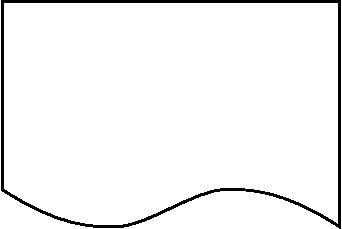
\includegraphics{styles/document.pdf}}}

\usepackage{epstopdf}

\tikzset{
  ciscorouter/.style={align=center,label={center:
      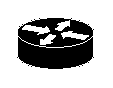
\includegraphics[]{styles/cisco/router.eps}
    },minimum width=0.9cm,minimum height=0.9cm}
}
\tikzset{
  ciscotap/.style={align=center,label={center:
      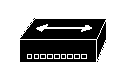
\includegraphics[]{styles/cisco/smallhub.eps}
    },minimum width=0.9cm,minimum height=0.9cm}
}

\usepackage{circuitikz}
\usepackage{multicol}
\newcommand*{\tabbox}[2][t]{\vspace{0pt}\parbox[#1][3.7\baselineskip]{1cm}{\strut#2\strut}}
\usepackage{float}
\usepackage{graphicx}
\usepackage{tabu}
\usepackage{lastpage}
\usepackage{lmodern}
\usepackage[toc,page]{appendix}
\usepackage[titles]{tocloft}
\usepackage{listings}
\usepackage{DejaVuSansMono}
\usepackage{tabularx}
\usepackage{fancyhdr}
\usepackage{cancel}
\setlength{\headheight}{15pt}
\pagestyle{fancyplain}
\usepackage{chngcntr}
\usepackage{footnote}
\makesavenoteenv{tabular}
\makesavenoteenv{table}
\counterwithout{footnote}{chapter}
\usepackage[hang,flushmargin,multiple]{footmisc}
\fancyhf{} % Ingen linje
% Skriv kapitelnavn som lowercase
\renewcommand{\chaptermark}[1]{\markboth{#1}{}}
\lhead[\fancyplain{}{\textit{\thechapter.\ \leftmark}}]{}
\rhead[]{\fancyplain{}{\textit{\leftmark\ \thechapter.}}}
\rfoot[]{\thepage}
\lfoot[\thepage]{}

\definecolor{lightgray}{gray}{0.90}
\newcommand{\colorbitbox}[3]{%
\rlap{\bitbox{#2}{\color{#1}\rule{\width}{\height}}}%
\bitbox{#2}{#3}}

\setcounter{tocdepth}{1}

%\renewcommand{\appendixname}{Bilag}
%\renewcommand{\appendixpagename}{Bilag}
%\renewcommand{\appendixtocname}{Bilag}

\usepackage{caption}
\captionsetup{font=footnotesize,labelfont=bf}
\captionsetup[figure]{labelfont=bf}
\usepackage{titlesec}
\titleformat{\chapter}{\normalfont\LARGE\bfseries}{\thechapter}{1em}{}
\titlespacing*{\chapter}{0pt}{-50pt}{20pt}
%\captionsetup[lstlisting]{labelfont=bf}
\usepackage{MnSymbol}
%\lstset{basicstyle=\scriptsize, tabsize=2, captionpos=b, frame=single}
\lstset{prebreak=\raisebox{0ex}[0ex][0ex]{\ensuremath{\rhookswarrow}}}
\lstset{breaklines=true, breakatwhitespace=true}
\renewcommand{\lstlistingname}{Code}

\lstset{
  language=c,
  basicstyle=\ttfamily\scriptsize,
  identifierstyle=\ttfamily,
  keywordstyle=\ttfamily,
  numbers=left,
  numbersep=5pt,
  xleftmargin=20pt,
  frame=tb,
  framexleftmargin=20pt,
  showstringspaces=false
}

\renewcommand*\thelstnumber{\arabic{lstnumber}:}

\DeclareCaptionFormat{mylst}{\hrule#1#2#3}
\captionsetup[lstlisting]{format=mylst,labelfont=bf,singlelinecheck=off,labelsep=space}


\usepackage{suffix}
\newcommand{\algoref}[1]{Algorithm~\ref{alg:#1}}
\newcommand{\appendixref}[1]{Appendix~-~\emph{\nameref{app:#1}}}
\newcommand{\appendixfigref}[2]{Appendix~\emph{\nameref{app:#1}~-~Figure~\ref{fig:#2}}}
\WithSuffix\newcommand\appendixref*[1]{Appendix~-~\emph{\nameref{app:#1}}}
%\newcommand{\@@appendixref}[1]{Appendix~\emph{\ref{app:#1}}}
\newcommand{\reqref}[1]{Req. \ref{req:#1_long}}
\newcommand{\reqrefnotext}[1]{Req. \ref{req:#1}}
\newcommand{\reqrefshort}[1]{\ref{req:#1_long}}
\newcommand{\reqrefshortnotext}[1]{\ref{req:#1}}
\captionsetup[subfigure]{labelformat=parens}
\newcommand{\subfigref}[1]{(\subref{fig:#1})}
\newcommand{\sectionref}[1]{Section~\emph{\ref{sec:#1}~\nameref{sec:#1}}}
\WithSuffix\newcommand\sectionref*[1]{Section~\emph{\ref{sec:#1}}}
\newcommand{\chapterref}[1]{Chapter~\emph{\ref{sec:#1}~\nameref{sec:#1}}}
\WithSuffix\newcommand\chapterref*[1]{Chapter~\emph{\ref{sec:#1}}}
\newcommand{\figref}[1]{Figure~\ref{fig:#1}}
\newcommand{\listingref}[1]{\lstlistingname~\ref{lst:#1}}
\newcommand{\tableref}[1]{Table~\ref{tab:#1}}
\newcommand{\theoremref}[1]{Theorem~\ref{th:#1}}
\newcommand{\equationref}[1]{Equation~\ref{eq:#1}}


\newcounter{req_counter}
\setcounter{req_counter}{1}

\makeatletter
\newcommand{\reqlabel}[2]{%
  \label{#1}
  \protected@write \@auxout {}{\string \newlabel {#1_long}{{\ref{#1} (#2)}{\thepage}{#2}{#1}{}}}%
  \hypertarget{#1}{#2}
}
\makeatother

\newcommand{\fullfigure}[3]{
  \begin{figure}[ht]
    \centering
    \includegraphics[width=.95\textwidth]{#1}
    \caption{#3}
    \label{fig:#2}
  \end{figure}
}

\newcommand{\fullfigurehere}[3]{
  \begin{figure}[H]
    \centering
    \includegraphics[width=.95\textwidth]{#1}
    \caption{#3}
    \label{fig:#2}
  \end{figure}
}

\newcommand{\fullfigureimport}[3]{
  \begin{figure}[ht]
    \centering
    \input{#1}
    \ifthenelse{\equal{#3}{}}{}{
      \caption{#3}
    }
    \ifthenelse{\equal{#2}{}}{}{
      \label{fig:#2}
    }
  \end{figure}
}

\newcommand{\largefigureimport}[3]{
  \begin{figure}[ht]
    \centering
    \scalebox{0.8}{\input{#1}}
    \ifthenelse{\equal{#3}{}}{}{
      \caption{#3}
    }
    \ifthenelse{\equal{#2}{}}{}{
      \label{fig:#2}
    }
  \end{figure}
}

\newcommand{\mediumfigureimport}[3]{
  \begin{figure}[ht]
    \centering
    \scalebox{0.66}{\input{#1}}
    \ifthenelse{\equal{#3}{}}{}{
      \caption{#3}
    }
    \ifthenelse{\equal{#2}{}}{}{
      \label{fig:#2}
    }
  \end{figure}
}

\newcommand{\smallfigureimport}[3]{
  \begin{figure}[ht]
    \centering
    \scalebox{0.50}{\input{#1}}
    \ifthenelse{\equal{#3}{}}{}{
      \caption{#3}
    }
    \ifthenelse{\equal{#2}{}}{}{
      \label{fig:#2}
    }
  \end{figure}
}

\newcommand{\tinyfigureimport}[3]{
  \begin{figure}[ht]
    \centering
    \scalebox{0.25}{\input{#1}}
    \ifthenelse{\equal{#3}{}}{}{
      \caption{#3}
    }
    \ifthenelse{\equal{#2}{}}{}{
      \label{fig:#2}
    }
  \end{figure}
}

\newcommand{\fullfigureimporthere}[3]{
  \begin{figure}[H]
    \centering
    \input{#1}
    \ifthenelse{\equal{#3}{}}{}{
      \caption{#3}
    }
    \ifthenelse{\equal{#2}{}}{}{
      \label{fig:#2}
    }
  \end{figure}
}

\newcommand{\fullfigureimporttop}[3]{
  \begin{figure}[t]
    \centering
    \input{#1}
    \ifthenelse{\equal{#3}{}}{}{
      \caption{#3}
    }
    \ifthenelse{\equal{#2}{}}{}{
      \label{fig:#2}
    }
  \end{figure}
}

\newcommand{\fullpagefigure}[3]{
  \begin{figure}[hbtp]
    \centering
    \includegraphics{#1}
    \caption{#3}
    \label{fig:#2}
  \end{figure}
}


\newcommand{\fullpagefigureimport}[3]{
  \begin{figure}[hbtp]
    \centering
    \input{#1}
    \caption{#3}
    \label{fig:#2}
  \end{figure}
}

\newcommand{\smallfigure}[3]{
  \begin{figure}[ht]
    \centering
    \includegraphics[width=.55\textwidth,height=.55\textwidth,keepaspectratio]{#1}
    \caption{#3}
    \label{fig:#2}
  \end{figure}
}

\newcommand{\smallerfigure}[3]{
  \begin{figure}[ht]
    \centering
    \includegraphics[width=.50\textwidth,height=.55\textwidth,keepaspectratio]{#1}
    \caption{#3}
    \label{fig:#2}
  \end{figure}
}

\newcommand{\tinyfigure}[3]{
  \begin{figure}[ht]
    \centering
    \includegraphics[width=.25\textwidth,height=.25\textwidth,keepaspectratio]{#1}
    \caption{#3}
    \label{fig:#2}
  \end{figure}
}


\newcommand{\mediumfigure}[3]{
  \begin{figure}[ht]
    \centering
    \includegraphics[width=.65\textwidth,height=.65\textwidth,keepaspectratio]{#1}
    \caption{#3}
    \label{fig:#2}
  \end{figure}
}

\newcommand{\largefigure}[3]{
  \begin{figure}[ht]
    \centering
    \includegraphics[width=.75\textwidth,height=.75\textwidth,keepaspectratio]{#1}
    \caption{#3}
    \label{fig:#2}
  \end{figure}
}

\newcommand{\largerfigure}[3]{
  \begin{figure}[ht]
    \centering
    \includegraphics[width=.85\textwidth,height=.85\textwidth,keepaspectratio]{#1}
    \caption{#3}
    \label{fig:#2}
  \end{figure}
}

\newcommand{\evenlargerfigure}[3]{
  \begin{figure}[ht]
    \centering
    \includegraphics[width=.99\textwidth,height=.95\textwidth,keepaspectratio]{#1}
    \caption{#3}
    \label{fig:#2}
  \end{figure}
}

\newcommand{\largestfigure}[3]{
  \begin{figure}[ht]
    \centering
    \includegraphics[width=1.05\textwidth,height=1.05\textwidth,keepaspectratio]{#1}
    \caption{#3}
    \label{fig:#2}
  \end{figure}
}


% \twofigures{width}{fig1name}{fig1label}{fig1caption}{fig2name}{fig2label}{fig2caption}{overall_label}{overall_caption}
\newcommand{\twofigures}[9]{
  \begin{figure}[H]
	\centering
	\begin{subfigure}[b]{#1\textwidth}
		\centering
		\includegraphics[width=\textwidth]{#2}
		\caption{#4}
        \label{fig:#3}
	\end{subfigure}
    \quad
	\begin{subfigure}[b]{#1\textwidth}
		\centering
		\includegraphics[width=\textwidth]{#5}
		\caption{#7}
        \label{fig:#6}
	\end{subfigure}
	\caption{#9}
    \label{fig:#8}
  \end{figure}
}

% \threefigures{width}{fig1name}{fig1caption}{fig2name}{fig2caption}{fig3name}{fig3caption}{fig4name}{fig4caption}{fig5name}{fig5caption}{overall_label}{overall_caption}
\newcommand{\threefigures}[9]{
  \begin{figure}[H]
	\centering
	\begin{subfigure}[b]{#1\textwidth}
		\centering
		\includegraphics[width=\textwidth]{#2}
		\caption{#3}
        \label{fig:#2}
	\end{subfigure}
    \quad
	\begin{subfigure}[b]{#1\textwidth}
		\centering
		\includegraphics[width=\textwidth]{#4}
		\caption{#5}
        \label{fig:#4}
	\end{subfigure}
    \quad
	\begin{subfigure}[b]{#1\textwidth}
		\centering
		\includegraphics[width=\textwidth]{#6}
		\caption{#7}
        \label{fig:#6}
	\end{subfigure}
	\caption{#9}
    \label{fig:#8}
  \end{figure}
}



% Bibliography
\bibliographystyle{IEEE}

\usepackage[footnote,draft,danish,silent,nomargin]{fixme}
\newcommand{\unit}[1]{~\text{#1}}
\newcommand{\rom}[1]{\uppercase\expandafter{\romannumeral #1}}

\newacronym{cnn}{CNN}{Convolutional Neural Network}
\newacronym{pascalvoc}{PASCAL VOC}{Pattern Analysis, Statistical Modelling and Computational Learning Visual Object Classes}
\newacronym{mscoco}{MS COCO}{Microsoft Common Objects in Context}
\newacronym{ilsvrc}{ILSVRC}{ImageNet Large Scale Visual Recognition Challenge}
\newacronym{svm}{SVM}{Support Vector Machine}
\newacronym{nms}{NMS}{Non-maximum Suppression}
\newacronym{map}{mAP}{Mean Average Precision}
\newacronym{roi}{RoI}{Region of Interest}
\newacronym{rpn}{RPN}{Region Proposal Network}
\newacronym{iou}{IoU}{Intersection-Over-Union}
\newacronym{ssd}{SSD}{Single Shot Detector}
\newacronym{yolo}{YOLO}{You Only Look Once}
\newacronym{fcn}{FCN}{Fully Convolutional Network}
\newacronym{rfcn}{R-FCN}{Region-based Fully Convolutional Network}
\newacronym{ion}{ION}{Inside-Outside Net}
\newacronym{rnn}{RNN}{Recurrent Neural Network}
\newacronym{tdm}{TDM}{Top-down Modulation}
\newacronym{fcis}{FCIS}{Fully Convolutional Instance-aware Segmentation}
\newacronym{ohem}{OHEM}{Online Hard Example Mining}
\newacronym{sgd}{SGD}{Stochastic Gradient Descent}
\newacronym{relu}{ReLU}{Rectified Linear Unit}
\newacronym{flops}{FLOPs}{Floating Point Operations}
\newacronym{ap}{AP}{Average Precision}
\newacronym{caffe}{Caffe}{Convolutional Architecture for Fast Feature Embedding}
\newacronym{iqa}{IQA}{Image Quality Assessment}
\newacronym{nr}{NR}{No-Reference}
\newacronym{live}{LIVE}{Laboratory for Image \& Video Engineering}
\newacronym{lcc}{LCC}{Pearson Linear Correlation Coefficient}
\newacronym{srocc}{SROCC}{Spearman Rank Order Coefficient}
\newacronym{ff}{FF}{Fast Fading}
\newacronym{bpp}{BPP}{Bits per Pixel}
\newacronym{dmos}{DMOS}{Difference Mean Opinion Score}
\newacronym{ar}{AR}{Average Recall}
\newacronym{friqa}{FR-IQA}{Full-Reference Image Quality Assessment}
\newacronym{nriqa}{NR-IQA}{No-Reference Image Quality Assessment}
%\makeatletter\@addtoreset{chapter}{part}\makeatother%

\usepackage[pdftex,
pdfauthor={Christoffer Bøgelund Rasmussen},
pdfsubject={Vision Graphics and Interactive Systems - Master's Thesis, Aalborg University},
pdftitle={ChristofferRasmussenMastersThesis},
pdfborder={0 0 0}
]{hyperref}

\usepackage{todonotes}
\newcommand{\unsure}[2][1=]{\todo[linecolor=red,backgroundcolor=red!25,bordercolor=red,#1]{#2}}
\newcommand{\change}[2][1=]{\todo[linecolor=blue,backgroundcolor=blue!25,bordercolor=blue,#1]{#2}}
\newcommand{\add}[2][1=]{\todo[linecolor=yellow,backgroundcolor=yellow!25,bordercolor=yellow,#1]{#2}}
\newcommand{\info}[2][1=]{\todo[linecolor=OliveGreen,backgroundcolor=OliveGreen!25,bordercolor=OliveGreen,#1]{#2}}
\newcommand{\improvement}[2][1=]{\todo[linecolor=Plum,backgroundcolor=Plum!25,bordercolor=Plum,#1]{#2}}
\newcommand{\thiswillnotshow}[2][1=]{\todo[disable,#1]{#2}}

\makeatletter
\renewcommand\part{%
  \if@openright
    \cleardoublepage
  \else
    \clearpage
  \fi
  \thispagestyle{empty}%
  \if@twocolumn
    \onecolumn
    \@tempswatrue
  \else
    \@tempswafalse
  \fi
  \null\vfil
  \secdef\@part\@spart}
\makeatother

\begin{document}

% FRONT PAGE
\lhead[\fancyplain{}{\textit{\leftmark}}]{}
\rhead[]{\fancyplain{}{\textit{\leftmark}}}
%\listoffixmes
\begin{titlepage}

\newcommand{\HRule}{\rule{\linewidth}{0.5mm}} % Defines a new command for the horizontal lines, change thickness here

\center % Center everything on the page

%----------------------------------------------------------------------------------------
%	TITLE SECTION
%----------------------------------------------------------------------------------------

\HRule \\[0.5cm]
{\LARGE \bfseries 
Master's Thesis
}\\[0.3cm]
\HRule \\[0.5cm]

%\frame{\includegraphics[scale=0.4]{frontpage.png}}

%----------------------------------------------------------------------------------------
%	AUTHOR SECTION
%----------------------------------------------------------------------------------------
\null
\vfill%[0.5cm]

\begin{minipage}[b]{0.4\textwidth}
\begin{flushleft} \large
\textbf{Authors:}\\
Christoffer Bøgelund Rasmussen\\
\emph{ }\\
\textbf{Supervisors:}\\
Kamal Nasrollahi\\
\end{flushleft}
\end{minipage}
~
\begin{minipage}[b]{0.4\textwidth}
\begin{flushright} \large
\textsc{\large Aalborg University}\\
\textsc{\large VGIS}\\ 
\textsc{\large 10th semester}\\
\textsc{\large Group 17gr1041}\\
\emph{ }\\
\textsc{\small TBA}\\
\end{flushright}
\end{minipage}

\end{titlepage}

\thispagestyle{empty}
\newpage
\cleardoublepage
\newpage
\thispagestyle{empty}

% SYNOPSIS
%undlader sidenummer
%fix test
\thispagestyle{empty}


\begin{wrapfigure}{r}{0.35\textwidth}
	\vspace{-80pt}
	\hspace{-60pt}
	\centering
	
\includegraphics{Sections/Introduction/logo}
\end{wrapfigure}
\begin{tabular}{p{7.5cm} p{8cm}}
	\tabbox{ 
	\mbox {
		\begin{minipage}{6 cm}
			\textbf{Title:}\\
      Internship Report - Navicon A/S\\
      \textbf{Subject:}\\
			Interactive Systems\\
			\textbf{Project period:}\\
      1/9-2016 to 23/12-2016\\
			\textbf{Project group:}\\
			16gr945\\
			\textbf{Participants:}\\
      Christoffer Bøgelund Rasmussen\\
      \\
			\\
			\textbf{Supervisor:}\\
      Kamal Nasrollahi\\
			\textbf{Printed copies:}\\
		  2\\
			\textbf{Number of pages: }\\
      TBA\\
			\textbf{Appendix media:}\\
			AAU digital exam zip file\\
			\textbf{Finished:}\\
      16/1-2017
		\end{minipage}
	}}
	&
	\tabbox[t]{
	\fbox {
		\begin{minipage}{6.5 cm}
TBA
\end{minipage}
	}}
\end{tabular}
\null
\vfill
\begin{center}
\textit{{\scriptsize The content of this report is freely available, but publication (with references) is only allowed with permission from the authors}}
\end{center}

\newpage
\thispagestyle{empty}

% PREFACE
\glsresetall
\section*{Preface}
This report documents an ninth semester internship report on the Vision, Graphics and Interactive Systems master programme at Aalborg University. The purpose of the report is to 
\add[inline]{add overview over purpose of report}
\section*{Reading Guide}
Tables, code listings and figures are numbered sequentially within each chapter. Citations are written as [x] where x denotes the reference number used in the bibliography. Code classes and functions are written as \lstinline{class} and \lstinline{function()}, respectively.\\
\unsure[inline]{check if reading guide is correct}

Additional files have been uploaded to the AAU Digital Exam. \add[inline]{include description of uploaded files}

\vfill
~\\
\makebox[8 cm]{\hrulefill}\\
Christoffer Bøgelund Rasmussen\\
~\\

\cleardoublepage
\pagenumbering{roman}
\renewcommand{\thepage}{\arabic{page}}% Arabic numerals for page counter
\thispagestyle{empty}
\tableofcontents
\printglossary[type=\acronymtype,nogroupskip,nonumberlist,title=Abbreviations]
\lhead[\fancyplain{}{\textit{\thechapter.\ \leftmark}}]{}
\rhead[]{\fancyplain{}{\textit{\leftmark\ \thechapter.}}}
\clearpage{\pagestyle{empty}\cleardoublepage}


% CHAPTERS
\chapter{Introduction}
\begin{comment}
	%%%%Overview%%%%
	- fundamental problem in CV
		- much work over previous decades
	- goal: find specific category in a given image
		- of interest by itself. Localise and classification
		- also a pre-requisite step to higher-level vision tasks
			- activity & event recognition, scene understanding, + find more
	- difficulties 
		- inter-class differences small
		- intra-class variations large
			- shape, pose, colour, texture, background, differences in illumination/viewpoint etc between images
	- GPU/deep learning advances have meant that performance is starting to become satisfactory for real-world use in scenarios requiring high precision and accuracy
		- autonomous vehicles, military, medicinal
	- much discussion of AI taking labor jobs
		- find articles and specific examples
			- elon musk, bill gates, etc (leaders of tech)
		- object detection needed
		- improvements still to be made before being completely realised
	- next section, overview of object detection definition, key task and challenges within. Also SOTA related work
\end{comment}


Object detection is a fundamental area of computer vision that has had a great amount of research over the past decades. The general goal of object detection is to find a specific object in an image. The specific object is typically from within a pre-defined list of categories that are of interest for a given use case. Object detection generally consists of two larger tasks; localisation and classification. It is assumed that the objects of interest are not already located in the image and as objects can vary in number of pixels depending on factors such as distance and scale, objects must be both localised in an image and classified accurately. Localisation is typically done by with a bounding-box indicating where a given object is in the image. However, other methods such as objects' centres and closed boundaries can also be used \cite{zhang}. Not only is object detection an important task in localising and classifying, it is also a necessary earlier step in larger computer vision pipelines. For example, object detection is needed within the tasks such as activity and event recognition, scene understanding, and robotic picking.

Object detection is a challenging problem due to both some large scale issues and minute differences. Firstly, there is the challenge of differentiating objects between classes. Depending on the problem at hand the sheer number of potential categories present can be into the thousands or tens of thousand. On top of this separate object categories can be both very different in appearance, for example an apple and an aeroplane, but separate categories can also be similar in appearance, such as dogs and wolves.

Current state-of-the-art within object detection is also within the realm of deep learning with \glspl{cnn}. This is exemplified with almost all leading entries in benchmark challenges such as \gls{pascalvoc} \cite{pascalvoc2012}, ImageNet \cite{imagenet}, and \gls{mscoco} \cite{mscoco} consisting of \gls{cnn}-based approaches. However, improvements are still needed before object detection can be used in real-world scenarios that require a high level of precision, accuracy, and performance. 

\section{Initial Problem Statement}

\begin{comment}
	- what are specific problems within object detection?
	- 
\end{comment}

An initial problem statement can be formed as follows: \\

\textit{How is object detection performed with \glspl{cnn}?} \\ \\
Based upon this, the following chapter will cover these challenges. On top of this, related work into current state-of-the-art object detection will be researched.
\label{sec:intro}

\chapter{Problem Analysis} \label{chap:problemanalysis}
\begin{comment}
	%%%%Overview%%%%
	- summary of object class recognition
		- reit challenges from introduction
		- reit of goals - categorisation/localisation
		- one class or multi?
		- show figure 2
			- discuss differences and similarities 
		- general implementation pipeline
	- key challenges - cite robustness/scalability
	- intro to older (non-CNN/deep) methods
		- find from survey
		- eg hand picked feature extractors/SVMS
		- sliding window approaches
		- DPM
	- CNN based methods - taken over since Alexnet (2012) on Imagenet
		- was this classification
		- extended to object detection (use classification network)
		- increase in complexity with CNNs, increase in time per window
			- overcome with region proposals
		- became a 2 step process
			1. find a number of region proposals where an object may be situated
			2. determine if a given proposal is a given pre-defined class
		- overview of proposal methods
			- grouping & window scoring
				- summary of both
			- should be accurate & have high repeatability (see why in dollar cite)
		- pipeline therefore:
			- with a given region proposal method apply deep-based classifier on regions
			- multiple current SOTA do this or similar
				- R-CNN, Fast R-CNN, Faster R-CNN (accurate but not real-time)
				- SSD, YOLOv2/YOLO9000, R-FCN 
					- alternatives to R-CNN 
						- often use some of the same methods (RPN)
				- best instance segmentation COCO 2016 - 2nd best bbox COCO 2016 (2016????)

- important that object detector is translation-invariant
by nature image-level classification favors translation invariance. A shift of an object inside an image should be indiscriminative
However, object detection needs to localise representations that are translation-variant to an extent. Translation of an object inside a candidate box should produce meaningful responses for describing how good candidate box overlaps object
CITE: R-FCN 2016

\end{comment}

This chapter will outline object detection and it's key challenges. This includes aspects within robustness, computational-complexity and scalability. Once completed the key works within object detection will be analysed, both current state-of-the-art and notable older methods.

\section{Object Detection}
As mentioned in \sectionref{intro}, object detection consists of two larger tasks; classification and localisation. Depending on the problem at hand, object detection can be split into two categories. If only a single class is of interest, such as detecting a specific traffic sign, the object detection task is denoted as class-specific detection. Whereas, the more general case when multiple classes are of interest in an image is denoted as multi-class detection \cite{zhang}. Key challenges such as \gls{pascalvoc}, ImageNet, and \gls{mscoco} are of the latter task. This thesis will be within the multi-class detection domain and take these challenges into account when analysing related works in \sectionref{sota} and determining the algorithm to be implemented and evaluated in \sectionref{methodoverview}. An analysis of these key challenges is done in \sectionref{challenges}. The goal of a detector is to output a list of labels from a predefined list of categories indicating which objects are present and where they are located in an image. Object detection has a number of related fields which share to common goal of categories relevant objects. This can be seen in \figref{objfields}. In all four instances the goal is to categorise the two objects person and skateboard, however, the difference lies in the level of localisation precision. In \figref{objcat}, object categorisation aims to only classify the objects in the image without providing any indication as to where the objects are located. Object class detection in \figref{objbb}, localises the classified objects with the use of bounding-boxes, where ideally the bounding-boxes are placed as tightly around the given object as possible. Figure-ground segmentation in \figref{objfig}, indicates localisation with a lasso outline around the objects. Finally, in \figref{objseg}, semantic-segmentation localises objects at a pixel-level classifying each pixel that is related to the given object. 


\add[inline]{correct section refs to above}

\begin{figure}[H]
    \centering
    \begin{subfigure}[b]{0.2\textwidth}
        \center
        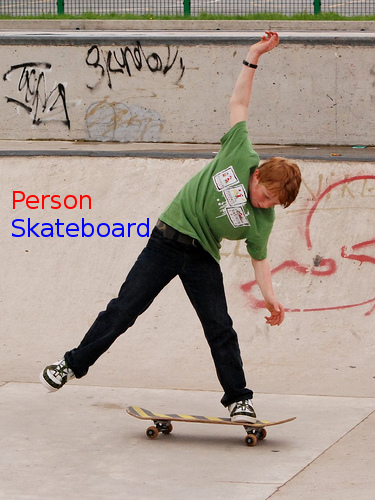
\includegraphics[width=\textwidth]{Figs/Problem/objfieldscat.png}
        \caption{}\label{fig:objcat}
    \end{subfigure}
    \begin{subfigure}[b]{0.2\textwidth}
        \center
        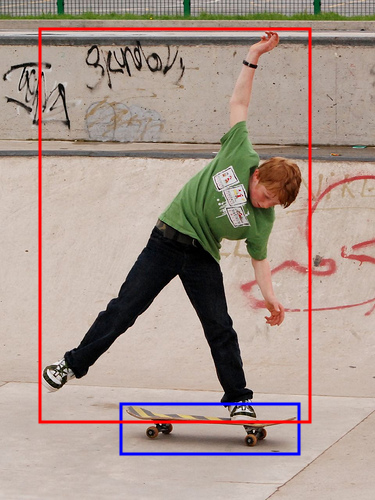
\includegraphics[width=\textwidth]{Figs/Problem/objfieldsbbox.png}
        \caption{}\label{fig:objbb}
    \end{subfigure}
    \begin{subfigure}[b]{0.2\textwidth}
        \center
        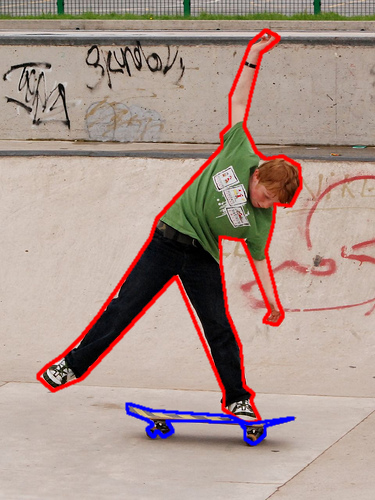
\includegraphics[width=\textwidth]{Figs/Problem/objfieldsfiguresegmentation.png}
        \caption{}\label{fig:objfig}
    \end{subfigure}
    \begin{subfigure}[b]{0.2\textwidth}
        \center
        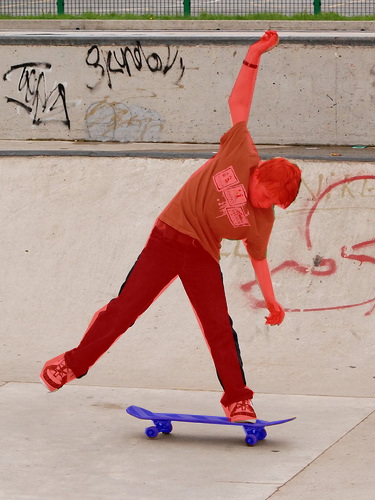
\includegraphics[width=\textwidth]{Figs/Problem/objfieldssegmentation.png}
        \caption{}\label{fig:objseg}
    \end{subfigure}
    \caption{Example of vision tasks related to object detection. All tasks have the common goal of categorising predefined objects. Methods are: object categorisation (a), object class detection (b), figure-ground segmentation (c), semantic Segmentation (d). Image and class labels taken from \gls{mscoco} \cite{mscoco}.}
    \label{fig:objfields}
\end{figure} 

A more recent example of segmentation is that of instance segmentation. Instance segmentation varies to semantic segmentation in that individual instances of objects are classified as such. If multiple instances of the same object is present, such as an image of a crowd with many people, in semantic segmentation all people will be given the same label as one large group. However, in instance segmentation the people are still given the same label but individual instances of a person is also found. This area of research within segmentation is relatively new, however, is beginning to become more popular in comparison to semantic segmentation. For example, the \gls{mscoco} segmentation challenge which has been held in 2015 and 2016 only accepts instance segmentation entries.


\section{Main Challenges}
The challenges of object detection can be split into two groups as per \cite{zhang}:

\begin{itemize}
	\item Robustness-related.
	\item Computational-complexity and scalability-related.
\end{itemize}

The following sections will outline the above.

\subsection{Robustness-related Challenges}

Robustness-related refers to the challenges in appearance within the both of intra-class and inter-class. Intra-class is the differences in appearance of objects which are of the same class. For example as seen in \figref{intra_ex}, all of the images belong to the superclass chair from the ImageNet training set \cite{imagenet}, however, vary greatly in their overall appearance. 

\begin{figure}[H]
    \centering
    \begin{subfigure}[b]{0.2\textwidth}
        \center
        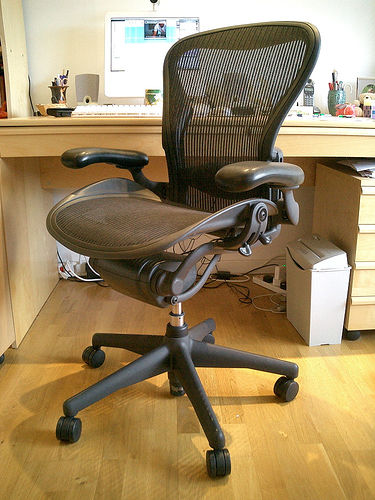
\includegraphics[width=\textwidth]{Figs/Problem/chair1.jpeg}
        \caption{}
    \end{subfigure}
    \begin{subfigure}[b]{0.2\textwidth}
        \center
        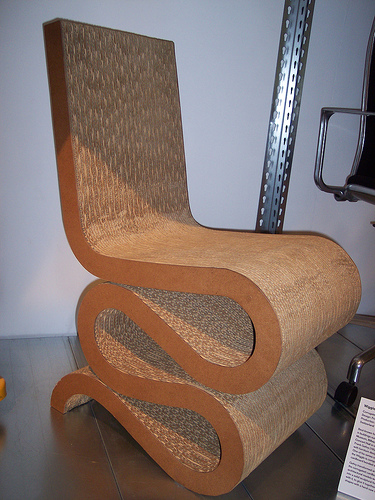
\includegraphics[width=\textwidth]{Figs/Problem/chair2.jpeg}
        \caption{}
    \end{subfigure}
    \begin{subfigure}[b]{0.2\textwidth}
        \center
        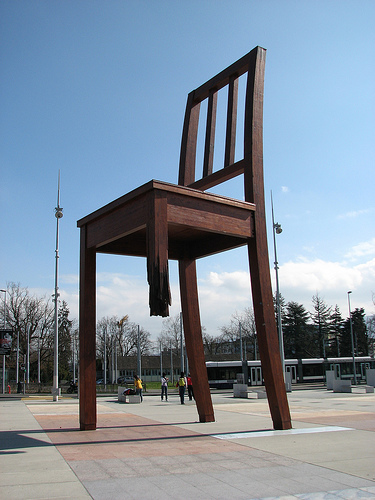
\includegraphics[width=\textwidth]{Figs/Problem/chair3.jpeg}
        \caption{}
    \end{subfigure}
    \begin{subfigure}[b]{0.2\textwidth}
        \center
        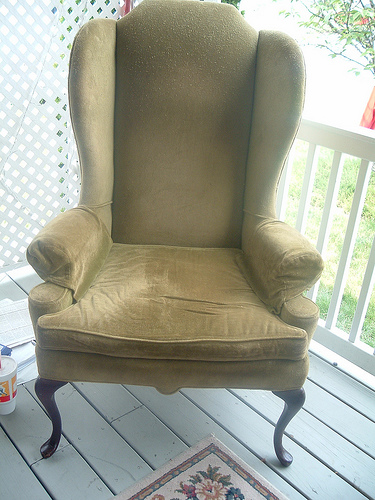
\includegraphics[width=\textwidth]{Figs/Problem/chair4.jpeg}
        \caption{}
    \end{subfigure}
    \caption{Examples of intra-class appearance variation. All images have the label chair in the ImageNet training set \cite{imagenet}.}
    \label{fig:intra_ex}
\end{figure} 

An object detection system must be able to learn \add[inline]{explanation that typically obj detection is supervised learning} the appearance variations that can occur intra-class. These variations can be categorised into two types as per \cite{schroff}:

\begin{itemize}
	\item Object variations.
	\item Image variations.
\end{itemize}

Object variations consist of appearance differences between instances of colour, texture, shape, and size. Image variations are differences not related to the object instances themselves but rather consist of conditions such as lighting, viewpoint, scale, occlusion, and clutter. Based upon these conditions the task of both classifying a given object as a given class but also differentiating the potentially largely varying objects into the same class challenging.
\unsure[inline]{unsure if to add explanation of structured and unstructured classes}

Robustness-related challenges can also occur with inter-class appearance differences. This refers to the differences between objects that are regarded as different categories. Challenges arise in scenarios where an object detector must decide if an instance is between classes that are very similar. For example using images and their respective classes from ImageNet \cite{imagenet}, in \figref{inter1} and \figref{inter2} the differences between the two examples are very similar, however, their class labels are different. In \figref{inter1a} and \figref{inter1b} the class labels are mini-bus and delivery truck respectively. In \figref{inter2a} and \figref{inter2b} the labels are white wolf and German shepherd. 

\begin{figure}[H]
    \centering
    \begin{subfigure}[b]{0.45\textwidth}
        \center
        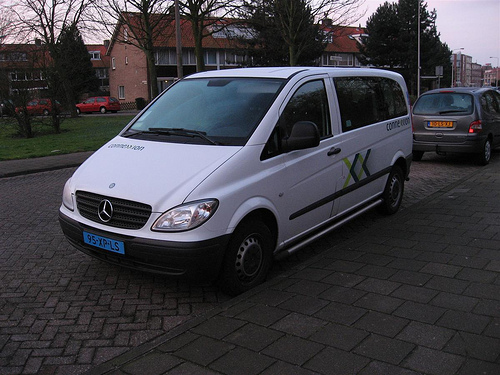
\includegraphics[width=\textwidth]{Figs/Problem/minibus.jpeg}
        \caption{}\label{fig:inter1a}
    \end{subfigure}
    \begin{subfigure}[b]{0.45\textwidth}
        \center
        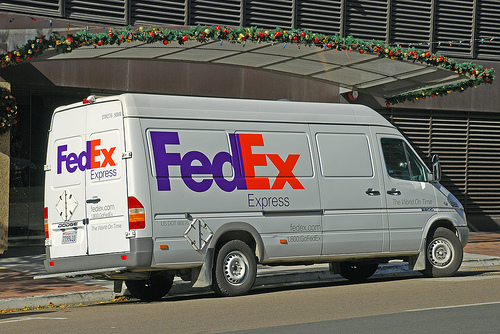
\includegraphics[width=\textwidth]{Figs/Problem/deliverytruck.jpeg}
        \caption{}\label{fig:inter1b}
    \end{subfigure}
    \caption{Examples of inter-class appearance variation. Both images are from the ImageNet training set \cite{imagenet} and have the labels mini-bus (a) and delivery truck (b).}
    \label{fig:inter1}
\end{figure} 

\begin{figure}[H]
    \centering
    \begin{subfigure}[b]{0.3\textwidth}
        \center
        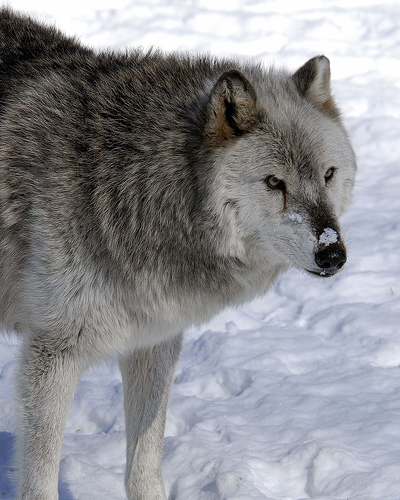
\includegraphics[width=\textwidth]{Figs/Problem/wolf.jpeg}
        \caption{}\label{fig:inter2a}
    \end{subfigure}
    \begin{subfigure}[b]{0.45\textwidth}
        \center
        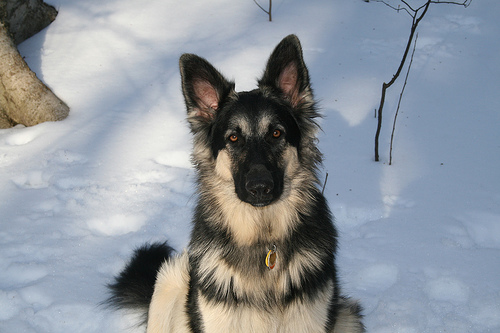
\includegraphics[width=\textwidth]{Figs/Problem/germanshepherd.jpeg}
        \caption{}\label{fig:inter2b}
    \end{subfigure}
    \caption{Examples of inter-class appearance variation. Both images are from the ImageNet training set \cite{imagenet} and have the labels White wolf (a) and German shepherd (b).}
    \label{fig:inter2}
\end{figure} 

It should be noted that this is a task-specific if inter-class appearance similarities is a problem or not. It can be argued that both the examples in \figref{inter1} and \figref{inter2} can be grouped into a larger superclass label if the given task does not require training of a model to such granularity. In both examples the classes stated are of the lowest class available in the overall hierarchy. ImageNet has labels available for each image along a larger array of classes and sub-classes. \figref{inter1_hierachy} visualises the granularity possible where both images belong to the superclass animal.

\begin{figure}[H]
    \centering
    \begin{subfigure}[b]{0.25\textwidth}
        \center
        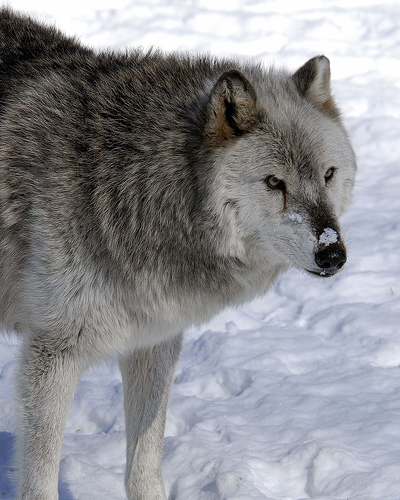
\includegraphics[width=\textwidth]{Figs/Problem/wolf.jpeg}
        \caption{}\label{fig:interhier1a}
    \end{subfigure}
    \begin{subfigure}[b]{0.20\textwidth}
        \center
        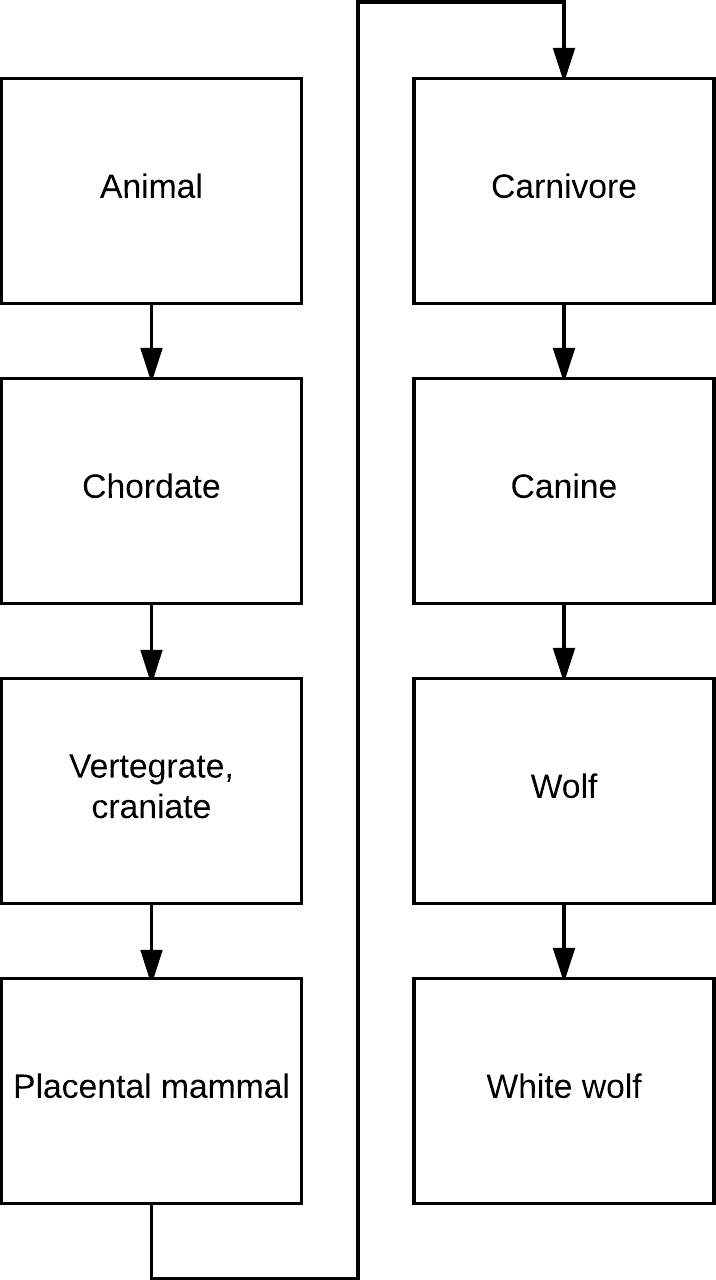
\includegraphics[width=\textwidth]{Figs/Problem/wolf_hier.png}
        \caption{}\label{fig:interhier1b}
    \end{subfigure}
        \begin{subfigure}[b]{0.25\textwidth}
        \center
        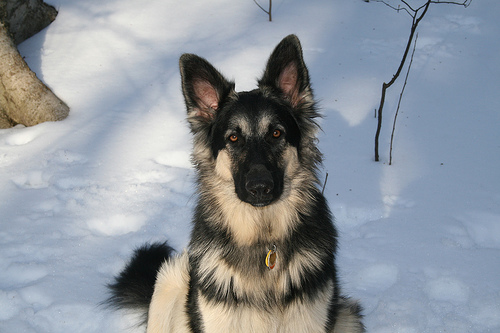
\includegraphics[width=\textwidth]{Figs/Problem/germanshepherd.jpeg}
        \caption{}\label{fig:interhier2a}
    \end{subfigure}
    \begin{subfigure}[b]{0.20\textwidth}
        \center
        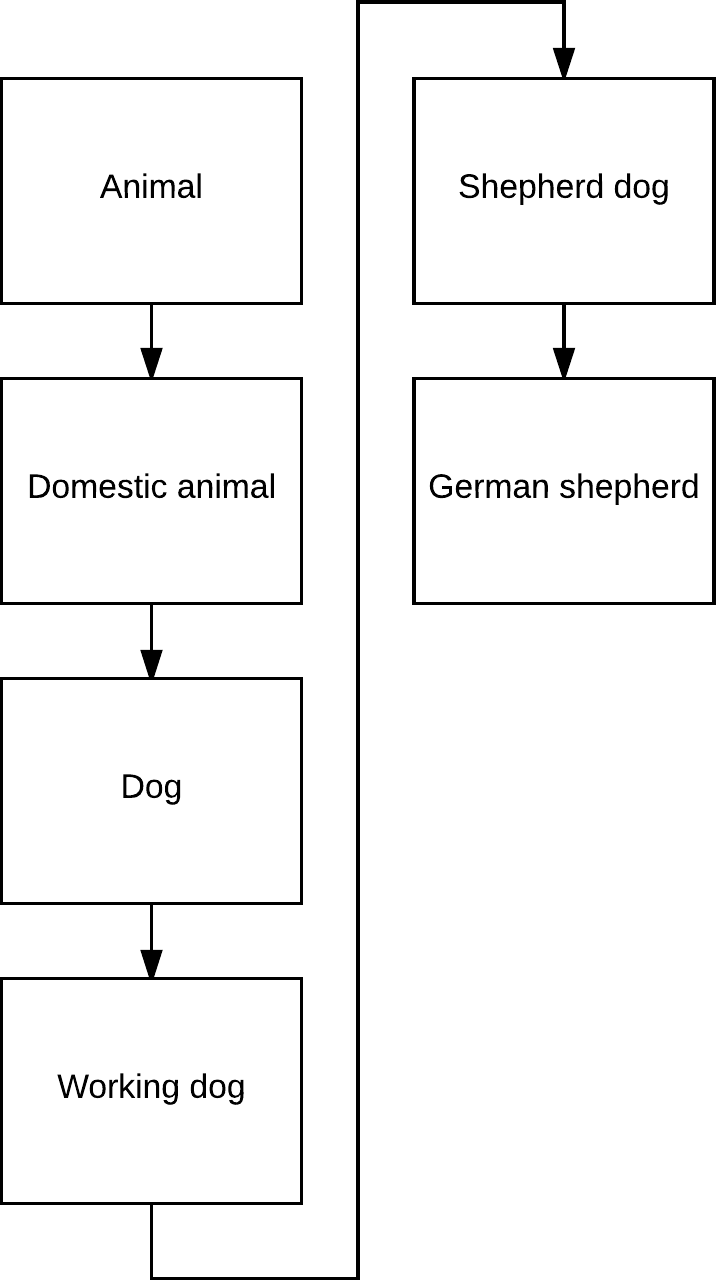
\includegraphics[width=\textwidth]{Figs/Problem/german_hier.png}
        \caption{}\label{fig:interhier2b}
    \end{subfigure}
    \caption{Visualisation of the hierarchy of potential classes for two examples in the ImageNet training set \cite{imagenet}.}
    \label{fig:inter1_hierachy}
\end{figure}

\subsection{Computational-complexity and Scalability-related Challenges}
The second challenge as per \cite{zhang} is related to the potential scale of object detection. When deciding on which type of model to use it must be complex enough to be able to capture the previously mentioned challenges both in inter- and intra-class. On top of this there is an extremely large number of potential classes in object detection. If the aim is to train a model to classify between an extreme number of classes then naturally a large number of images are also needed for each category. The large number of images need also to be representative enough in training to capture the necessary visual features to generalise on non-training images. In 2016 the ImageNet object detection challenge there is a total of 200 object categories, with 456,567 images comprising the training set. Therefore, a complex enough model is needed in order to learn and generalise on such a dataset but this of course places high requirements on the amount of training needed.

Issues can also arise over time when designing an object detection system.  Over time the visual appearance of an object can change, which is very difficult to take into account when training a model. For example, the visual appearance of televisions have changed greatly in the past century. If a system were only to be trained on images from an earlier time period it may not be able to generalise on new instances. Therefore, it is important that a model is able to be updated as the appearance of objects change. On top of this, new categories of objects can come to fruition which may needed to be added to a model. 

\section{Implementation Outline}
As per \cite{zhang} the steps in the general pipeline for an object detection system is as follows:

\begin{enumerate}
	\item Find all possible object regions in the image.
	\item Determine if the regions correspond to any of the predefined categories.
	\item Evaluate all responses from step 2 to determine final detections.
\end{enumerate}



\section{Benchmark Datasets}
This section will outline some of the commonly used object detection datasets. This will include their purpose and the general setup.


\subsection{PASCAL Visual Object Classes Challenge}
The \gls{pascalvoc} challenge \cite{pascalvoc2012} was held yearly between 2005 to 2012 and provided datasets for benchmarking within vision tasks of visual object category recognition and detection. Between that time period is was considered the top benchmark for the respective challenges. While being an annual competition, \gls{pascalvoc} evaluation in state-of-the-art literature is most often performed on data from the years 2007 and 2012. The competition saw a large shift in the former year as the number of classes increased from 10 to 20, in turn also significantly increasing the total amount of data. Additional data was added individually for the various recognition tasks between 2007 and 2012 and the performance metric was altered slightly between this time period, however, the overall ecosystem remained largely the same from 2007 until the competition's end. This section will be largely based upon the two retrospective papers, \cite{pascalvoc2010} and \cite{pascalvoc2015}, published by authors who were involved in the challenge and for the most part will be in respect to the challenge after 2007.
\\\\
Images were obtained from the website flickr \cite{flickr} with the aim in mind to collect natural images for the recognition challenges. Ideally the dataset was to contain a significant level of visual variability in regards to object size, orientation, pose, illumination, position, and occlusion. A total of 20 classes were present in the 2007 challenges and these remained the same until 2012. The classes can be considered as a part of a taxonomy with 4 main branches, where each has finer-grain objects in sub-classes. The 20 classes and the branching taxonomy can be seen in \tableref{vocclasses}.


\begin{table}[h]
\centering
\caption{Taxonomy of the 20 classes introduced in VOC2007.}
\label{tab:vocclasses}
\begin{tabular}{llll}
\hline
Vehicles & Household & Animals & Other \\ \hline
Aeroplane                      & Bottle                         & Bird                         & Person                     \\
Bicycle                        & Chair                          & Cat                          &                            \\
Boat                           & Dining table                   & Cow                          &                            \\
Bus                            & Potted plant                   & Dog                          &                            \\
Car                            & Sofa                           & Horse                        &                            \\
Motorbike                      & TV/Monitor                     & Sheep                        &                            \\ \hline
Train    &  &  &  \\ \hline
\end{tabular}
\end{table}

A total of 500,000 potential images were collected randomly based upon different combinations of queries for a given class. For example of class bird, potential queries were bird, birdie, birdwatching, nest, sea, aviary, birdcage, bird feeder, and bird table. Of these potential images the majority were discarded for potential annotation due to not meeting the considerations of visual variability mentioned earlier. The annotation process was completed by a team from the University of Leeds based upon strict guidelines. The aim was to ensure that the annotations resulted in a consistent, accurate, and exhaustive dataset. The annotations are stored in XML format which contains the following information:

\begin{itemize}
	\item Class: one of the 20 shown in \tableref{vocclasses}.
	\item Bounding box: axis-aligned bounding-box around the visual extent of the object.
	\item Viewpoint: viewpoint to the object.
	\item Truncation: whether or not object is truncated. An object is truncated when the bounding-box does not cover the full extent of the object. Truncation can occur if the object extends outside the image or is partially occluded.
	\item Difficult: A subjective evaluation on if the object is difficult to detect. This is determined based on object size, illumination, or image quality.
\end{itemize}

An example of the XML format for the object chair can be seen in Code \ref{lst:xml_ex} and its corresponding image in \figref{xml_eximg}. 

\begin{lstlisting}[language=xml,caption={Example of XML annotation for the object chair.}
\label{lst:xml_ex}]
<object>
    <name>chair</name>
    <pose>Rear</pose>
    <truncated>0</truncated>
	<difficult>0</difficult>
	<bndbox>
		<xmin>263</xmin>
		<ymin>211</ymin>
		<xmax>324</xmax>
		<ymax>339</ymax>
	</bndbox>
</object>
\end{lstlisting}

\begin{figure}[H]
  \centering
    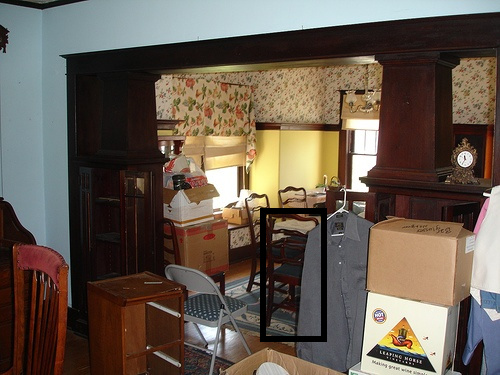
\includegraphics[width=0.7\textwidth]{Figs/Techanal/000005.jpg}
    \caption{Image from the \gls{pascalvoc} 2007 dataset. The bounding box represents the annotated XML data shown in Code \ref{lst:xml_ex}.}
    \label{fig:xml_eximg}
\end{figure}

Of the 500,000 potential images, 9,963 were annotated for the VOC2007 challenges based upon the annotation guidelines. \gls{pascalvoc} datasets is split into two subsets; \lstinline{trainval}, consisting of training and validation data and \lstinline{test}, consisting of the testing data. A histogram showing the frequency of an object class in an image and the total number of objects for the VOC2007 dataset can be seen in \figref{vochist07}.

\begin{figure}[H]
  \centering
    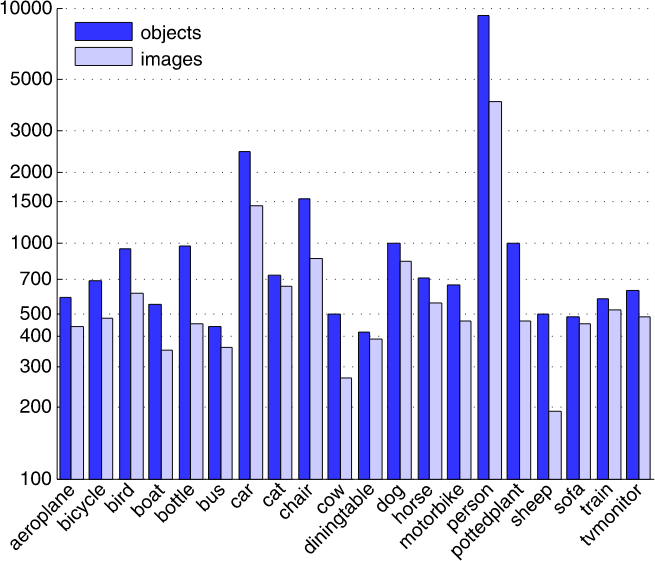
\includegraphics[width=0.5\textwidth]{Figs/Techanal/vochist07.png}
    \caption{Image from the \gls{pascalvoc} 2007 dataset. The bounding box represents the annotated XML data shown in Code \ref{lst:vochist07}.}
    \label{fig:vochist07}
\end{figure}


Evaluation of a object detector on \gls{pascalvoc} is based upon \gls{ap} which summarises the precision and recall of detections. The metric requires that for each detection both a bounding-box and an associated confidence. With these a precision/curve can be calculated and the overall \gls{ap} for the curve represents the performance of the detector. By altering the threshold corresponding to the confidence of each detection a precision and recall curve can be calculated and the \gls{ap} summarises the shape of the this. Precision is the number of true positives in relation to both true positives and false positives. Whereas, recall is the number of true positives in relation to all detections. However firstly, a detection must be classified as either a true or false positive. This is determined by measuring the bounding-box overlap between the detection and ground truth annotation. In \gls{pascalvoc} a bounding box is a true positive if the overlap is above 50\% according to the following calculation:

\begin{equation}\label{pascalBB}
	a_o = \frac{area(B_p \bigcap B_{gt})}{area(B_p \bigcup B_{gt})}
\end{equation}
 
where $B_p \bigcap B_{gt}$ is the intersection of the predicted bounding box and the ground truth and $B_p \bigcup G_{gt}$ is the union between the two. It should also be noted that for a given ground truth object it is only possible to have one true positive detection. If multiple detections satisfy Equation \ref{pascalBB} the remaining will be denoted as a false positive. Now that detections can be as classified as either a true or false positive \gls{ap} can be calculated. Before 2007, in \gls{pascalvoc} this was calculated as the mean precision at eleven equally space recalls [0, 0.1, ..., 1] by:

\begin{equation}
	AP = \frac{1}{11} \sum_{r\epsilon[0, 0.1, ..., 1]}p_{interp}(r)  
\end{equation}

where $r$ is the recall and $p_{interp}$ is the interpolated precision.
\add[inline]{explanation of interpolated precision}
\add[inline]{explanation of new metric}

\subsection{ImageNet Large Scale Visual Recognition Challenge}
\gls{ilsvrc} is an extremely large benchmark in object recognition. The challenge has been held since 2010 with multiple challenge tasks such as image classification, scene recognition and object detection. Currently, in 2017 the only challenges being held are object detection in both images and video. The aim of \gls{ilsvrc} was to create an image recognition challenge on such a scale that had not been previously seen. Before this, the main challenge was \gls{pascalvoc} with 20 categories in the object detection challenge. \gls{ilsvrc} has 200 classes, roughly 500,000 annotated positive and negative images and just under 500,000 annotated objects in the positive examples. Once again, the goal of an algorithm is to learn object detection towards to 200 classes and return a bounding-box with an associated confidence for each object detected in an image.
\\\\
Creating such a large dataset is a difficult and cumbersome task. The majority of images come from another \gls{ilsvrc} challenge of single-object localisation, where the aim was to only return a single object detection. Additional images were supplemented from Flickr queries. Examples of images from the dataset can be seen in \figref{imagenet_ex}.


\begin{figure}[H]
    \centering
    \begin{subfigure}[b]{0.4\textwidth}
        \center
        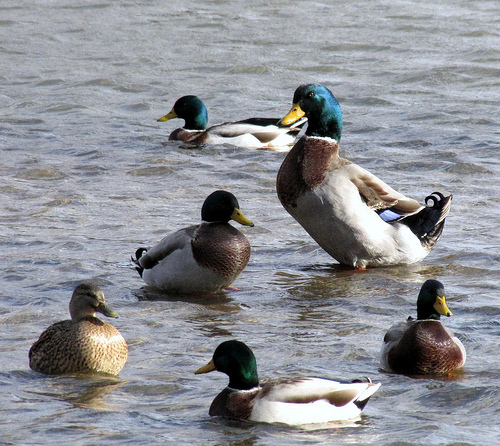
\includegraphics[width=\textwidth]{Figs/Problem/in1.jpeg}
        \caption{}\label{}
    \end{subfigure}
    \begin{subfigure}[b]{0.4\textwidth}
        \center
        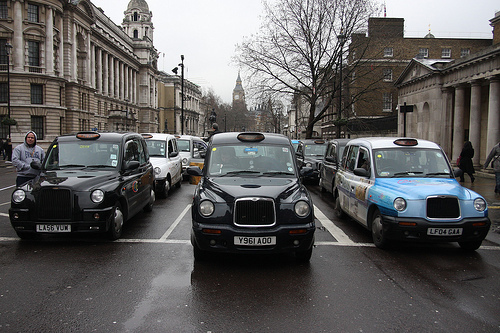
\includegraphics[width=\textwidth]{Figs/Problem/in2.jpeg}
        \caption{}\label{}
    \end{subfigure}
    \caption{Example of images in the \gls{ilsvrc} object detection challenges.}
    \label{fig:imagenet_ex}
\end{figure} 

Evaluation of detections was inspired by the \gls{ap} metric used in \gls{pascalvoc}. Again detections are determine to be correct or incorrect based on if the \gls{iou} is above 0.5. 
While being a challenging dataset in terms of the number of classes present, the object sizes and number of objects is similar to that of \gls{pascalvoc}. Next will be an explanation of a new benchmark that addresses such challenges.



\subsection{Microsoft Common Objects in Context}
\gls{mscoco} \cite{mscoco} is a relatively new dataset within the realm of object recognition appearing in 2015. \gls{mscoco} holds competitions in object detection and segmentation. The object detection challenge is similar to \gls{pascalvoc}, in that detections must be shown using bounding-boxes. However, for the segmentation challenge \gls{mscoco} requires the results to be of more challenging instance form rather than semantic. The creators of the dataset had three core research problems they wanted to be present, these include:

\begin{enumerate}
	\item Detecting non-iconic views of objects.
	\item Contextual reasoning between objects.
	\item Precise 2-dimensional localisation of objects.
\end{enumerate}

The first problem is present by having object instances in images that are closer to everyday scenarios. Iconic views of objects are when the instance is near the centre of the image, is unobstructed and taken in a controlled scenario. Objects taken in such conditions are much easier to detect but practical applications are limited. Therefore, non-iconic views of objects are collected by having images that can have background or other objects present, objects being partially occluded and being amongst clutter. By having a dataset of non-iconic views, the second research problem is addressed as objects are in scenarios where context with respect to the scene can be used. Finally, a higher level of precision is provided in the \gls{mscoco} segmentation challenge. As mentioned, results are required to be instance and pixel-wise. Therefore, the objects in the dataset are annotated precisely at a pixel-level but also with coarser bounding-boxes. These goals resulted in a dataset has a total of 91 object classes of which 82 have more than 5,000 labelled instances. Considerably higher that that of \gls{pascalvoc}. In addition to having a large number of classes the number of object instance per image is also relatively high. On average there is 7.7 instances per image, considerably higher than \gls{pascalvoc} with 2.3 and ImageNet with 3.0. 
\\\\
The object classes chosen are similar to those in \gls{pascalvoc}, where the categories should represent a common objects that are relevant to practical applications. Also the categories should be such that a high number of images that respect the core research problems can be found. The 91 categories were chosen to be at a higher-level of taxonomy such that they would be the commonly used label by a typical person. The categories and number of instances in each can be seen in \figref{cocoinstances}.

\begin{figure}[H]
  \centering
    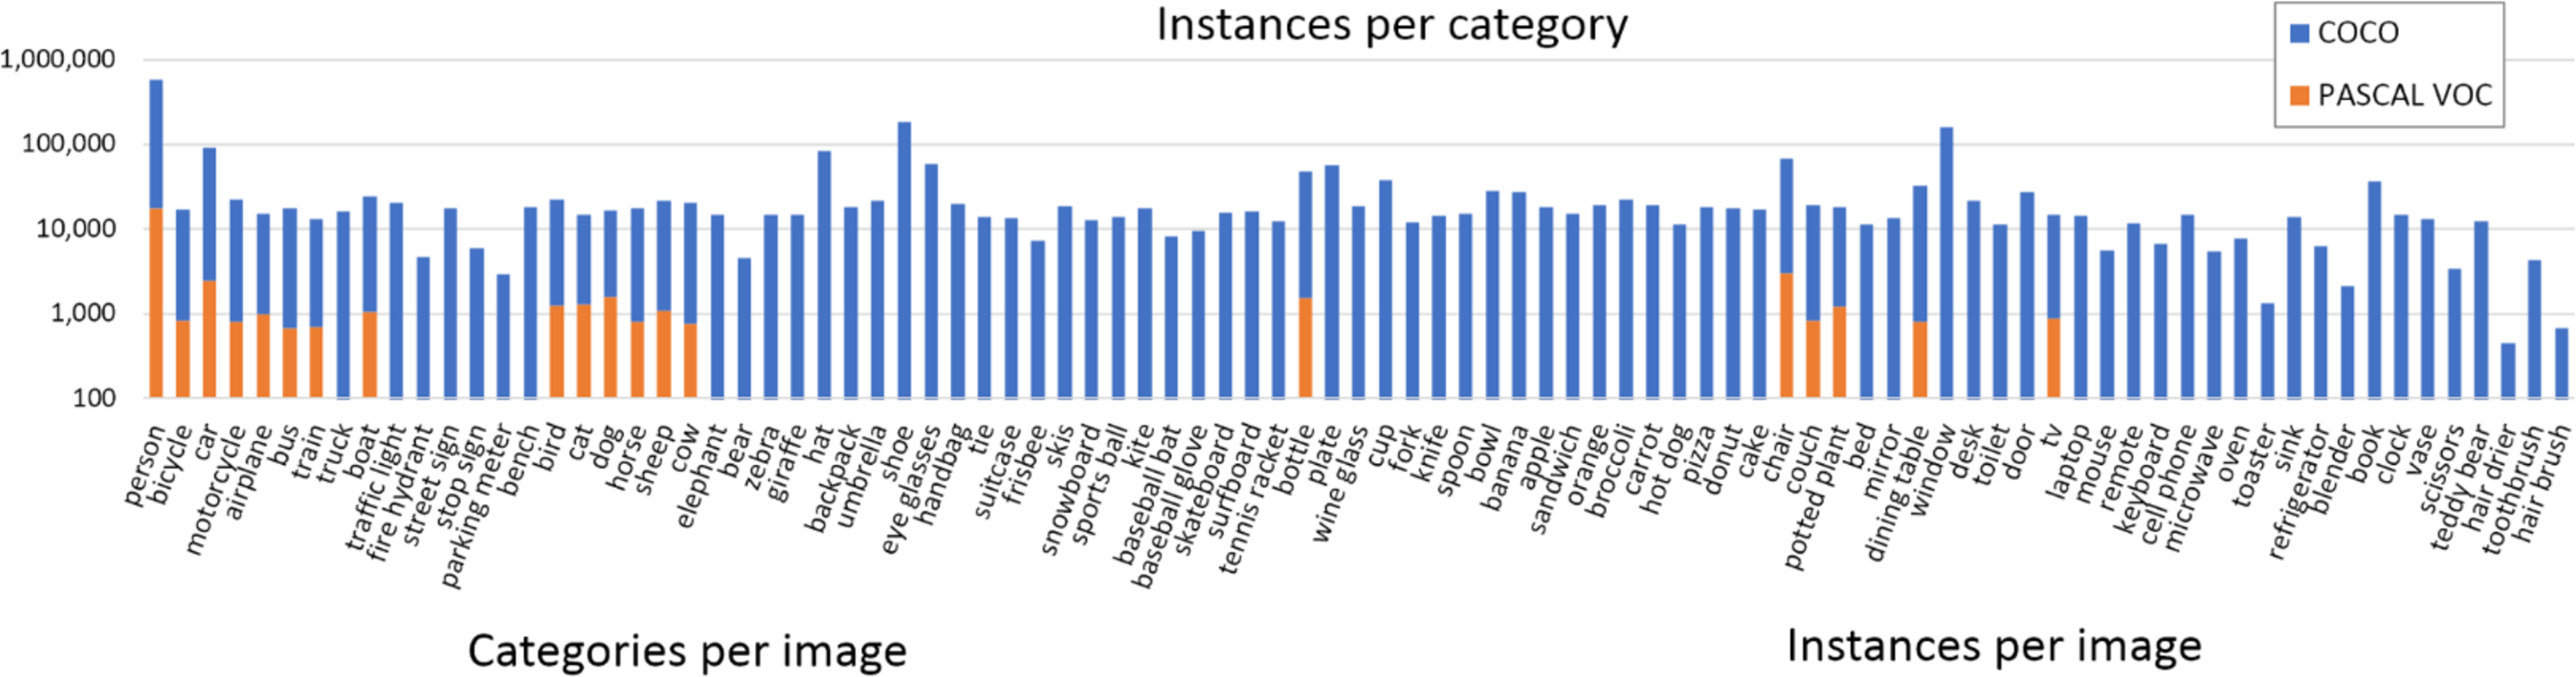
\includegraphics[width=1.0\textwidth]{Figs/Problem/mscoco_cats.pdf}
    \caption{Object categories and number of instances in each in the \gls{mscoco} dataset \cite{mscoco}.}
    \label{fig:cocoinstances}
\end{figure}


The image collection process was done using queries through Flickr inspired by the \gls{pascalvoc} method of collection. Having only a single categories as a query resulted in higher chances of iconic views, therefore multiple categories were used to collect images. Once collected and annotated the total number of images in the 2015 release was 328,000, split as 165,482 for training, 81,208 validation and 81,434 for testing.
\\\\
Apart from having a larger number of categories and there being a large number of instance per image (7.7), there are also other items that make this dataset more challenging. Firstly, the number of categories per image is larger than \gls{pascalvoc}, with 3.5 compared to 1.7. Additionally, the dataset is made up of much smaller images which are typically more difficult to detect. Roughly 65\% of object instances make up only 4-6\% of the total image size. This is in comparison to \gls{pascalvoc} at roughly 45\%.
\\\\
\gls{mscoco} uses 12 metrics to evaluate the performance of object detection, where 6 are variants of \gls{ap} and the remaining 6 variants of \gls{ar}. The \gls{ap} metric is calculated in the same manner as in \gls{pascalvoc}, however, the primary metric is also averaged over multiple \glspl{iou}. In \gls{pascalvoc} \gls{ap} is only calculated at \gls{iou}=0.5, however, in \gls{mscoco} \gls{ap} is average in the range of [0.50, 0.95] at intervals of 0.05. The \gls{mscoco} \gls{ap} is also evaluated on detections across ground truth image scales, as the number of small objects in the dataset is as mentioned relatively high. The scales covered is \gls{ap} for small objects that have a ground truth bounding-box are less than $32^2$ pixels, medium objects area between $32^2$ and $96^2$, and large objects with area above $96^2$. Apart from the primary metric and the three image scales, \gls{ap} is also calculated at two fixed \glspl{iou}. Firstly, at \gls{iou} 0.50 which results in the same metric as in \gls{pascalvoc} and at relatively strict \gls{iou} of 0.75. The \gls{ar} metric is also average across multiple \glspl{iou}, but also measure at a limitation of the maximum number of detections per image. This makes up three \gls{ar} metrics where maximum detections are 1, 10 and 100 per image. Finally the remaining three metrics evaluate the \gls{ar} across the same object scales mentioned earlier.
\begin{comment}
	- CNN approaches
	- R-CNN - fast - faster
	- SSD
	- R-FCN
	- YOLO (speed)	
\end{comment}

\section{Related Work}
One of the first methods to show that \glspl{cnn} could significantly improve object detection was that of R-CNN \cite{rcnn}. The method obtains the name R-CNN based upon a \gls{cnn} is used on regions of the image. Many earlier object detection approaches were used in a sliding window fashion testing all areas of an image. This can lead to a huge amount of potential testing windows especially if the object detection is done at a multitude of different scales. The method was heavily inspired by the AlexNet model that started the deep learning renaissance in 2012 by winning classification challenge in the \gls{ilsvrc}. The authors of R-CNN aimed to show that the advances in classification with a model such as AlexNet could also be done in object detection. In R-CNN the model is used as a feature extractor from which a class-specific linear \gls{svm} can be trained on top of. The AlexNet-based feature extractor is firstly pre-trained on a large dataset designed for classification, in this case the training set from \gls{ilsvrc} 2012. This pre-trained model is then adapted to the new domain of object detection by fine-tuning the model accordingly. In this instance the authors fine-tuned warped training instances from the \gls{pascalvoc} dataset. The AlexNet model was also altered to classify the 20 classes present in \gls{pascalvoc} rather than the 1000 classes in \gls{ilsvrc}. The pipeline of the R-CNN is split into 3 modules:

\begin{enumerate}
	\item Region proposals.
	\item Feature extraction.
	\item Class-specific linear \glspl{svm}.
\end{enumerate}

In this first module, region proposal, there is a large number of choices of methods to produce a suitable number of windows in comparison to a sliding window approach. R-CNN is agnostic to the region proposal method chosen and in the original work SelectiveSearch \cite{selectivesearch} is used. Module two, as explained earlier, is the use of a \gls{cnn} as a feature extractor. This is in the form of a 4096-dimensional feature vector from the domain-specific \gls{pascalvoc} trained AlexNet model. These feature vectors are used in the third module, class-specific linear \glspl{svm}. In the case of \gls{pascalvoc} a total of 21 \glspl{svm} are trained, one for each of the 20 classes in the challenge and one for a background class. The training of the \glspl{svm} is done by forward propagating a large number of both positive and negative region proposals found with SelectiveSearch and storing each 4096-dimensional feature vector to disk. After this the appropriate labels are applied to each vector and a linear \gls{svm} is optimised for the 21 classes. At test time, for a given image SelectiveSearch is used to produce around 2000 proposals. Each of the proposals are propagated through the network to extract their respective feature vectors. Each feature vector is then tested against every \gls{svm} to produce a score for each class. Finally greedy \gls{nms} is applied to remove overlapping detections. The approach outlined in R-CNN produced a significant improvement in object detection with an improvement of roughly 13\%, compared to previous state-of-the-art methods, to an overall 53.7\% \gls{map} on the \gls{pascalvoc} 2010 test set. Similar results were also found on the \gls{pascalvoc} 2011/12 set with \gls{map} of 53.5\%. Despite the significant improvements with a \gls{cnn}-based method on region proposals there are still issues with the R-CNN. Firstly, the testing time per image is very slow at roughly 47 seconds on an Nvidia K40 GPU. Also extracting features for each proposal in order to train the \glspl{svm} takes a large amount of disk space and may not be feasible on all hardware configurations. Finally, as the R-CNN is made up of 3 modules the training is done in a multi-stage manner rather than end-to-end. Therefore, the loss calculating when optimising the \glspl{svm} are not used to update the \gls{cnn} parameters.
\\\\
The R-CNN method was improved the following year with Fast R-CNN \cite{fastrcnn} and aimed to improve speed and accuracy. One of the significant changes is that the detection training done is now end-end rather than in the multi-stage pipeline in R-CNN. Due to this the large requirements of disk space due to feature caching is no longer required. The Fast-RCNN method takes both an image and a set of pre-computed object proposals. A \gls{cnn} forward propagates the entire image, rather than individual proposals in R-CNN, through several convolutional and max-pooling layers to produce a feature map. Features are extracted for each proposal in their corresponding location in the computed feature map with a \gls{roi} pooling layer. The \gls{roi} feature is calculated by splitting the $h \times w$ proposal into $H \times W$ sub-windows of size $h/H \times w/W$. Where $h$ and $w$ is the height and width respectively of a proposal. $H$ and $W$ are hyper-parameters specifying the fixed spatial extent of the extracted feature. Each sub-window has max-pooling applied and with the resulting value being placed in the corresponding output cell. Once the \gls{roi} pooling layer has been applied to a pre-computed object proposal the forward pass continues through two fully-connected layers followed by two sibling output layers. The sibling outputs are a softmax classification layer that produces probabilities for the object classes and another layer for bounding-box regression. These two layers replace the respective external modules in R-CNN and make it possible to train the entire detection network in a single-stage. As in R-CNN, pre-training a \gls{cnn} on a large classification dataset and fine-tuning towards detection and a specific object classes is done in a similar fashion. In R-CNN, the only deep network used was AlexNet \cite{alexnet}, however, in Fast R-CNN the authors experiment with networks of different size. It was found that the deeper network VGG16 \cite{vgg16} for computing the convolutional feature map gave a considerable improvement in \gls{map}. For a fair comparison of results against R-CNN, its \gls{cnn} was the same pre-trained VGG16 network. The \gls{map} results on \gls{pascalvoc} 2007, 2010, and 2012 compared against R-CNN can be seen in \tableref{fastresults}. 

\begin{table}[]
\centering
\caption{A comparison of R-CNN and Fast R-CNN \gls{pascalvoc} \gls{map} results on the test set from 2007, 2010, and 2012.}
\label{tab:fastresults}
\begin{tabular}{|l|l|l|l|}
 \hline
           & 2007 & 2010 & 2012 \\ \hline
R-CNN      & 66.0 & 62.9 & 62.4 \\ 
Fast R-CNN & \textbf{66.9} & \textbf{66.1} & \textbf{65.7} \\ \hline
\end{tabular}
\end{table}

However, as the name Fast R-CNN implies the main improvement is the speed in respect to both training and testing. By computing a convolutional feature map for an entire image rather than per object proposal the number of passes in the network is lowered significantly. Also by makign the detection training end-to-end with the two sibling layers lowers the training time needed. An overview of time spent training and testing both Fast R-CNN and R-CNN with a VGG16 \gls{cnn} can be seen in \tableref{fastspeed}.

\begin{table}[]
\centering
\caption{Speedup between R-CNN and Fast R-CNN in regards to both training and testing. Both methods are train a VGG16 network for object detection.}
\label{tab:fastspeed}
\begin{tabular}{|l|l|l|}
\hline
                          & R-CNN & Fast R-CNN \\ \hline
Train time (hours)        & 84    & \textbf{9.5}        \\ 
Train speed-up             & 1x    & \textbf{8.8$\times$}       \\ \hline
Test time (seconds/image) & 47.0  & \textbf{0.32}       \\ 
Test speed-up              & 1x    & \textbf{146$\times$}       \\ \hline
\end{tabular}
\end{table}

While Fast R-CNN provided improvements in both accuracy and speed, the increase in speed is only in relation to the actual object detection and assumes that the region proposals are pre-computed. Therefore, there is still a significant bottleneck per image as a region proposal method can typically take a couple of seconds. 
\\\\
The region proposal bottleneck was addressed in the third iteration of the R-CNN network with Faster R-CNN \cite{fasterrcnn}. In this method it was shown how to compute region proposals with a deep \gls{cnn} with a part of the network called \gls{rpn}. A \gls{rpn} shares the convolutional layers and feature map used for computing features with \gls{roi} pooling in Fast R-CNN. As this deep network is already being computed on the entire image for the classification pipeline the added time for proposals using the \gls{rpn} is negligible (10ms) in comparison to a method such as SelectiveSearch. Apart from the change in how region proposals are computed there is no change in comparison to Fast R-CNN. 
An \gls{rpn} takes the convolutional feature map as input and returns a number of object proposals. Each proposals is fed into two sibling layers, similar to that in Fast R-CNN, one layer scoring how likely to be an object or background and another performing bounding-box regression. The proposals are found through a method denoted as anchors. At each sliding-window location $k$ proposals are with anchors that are user-defined reference boxes for how an object proposal may be formed. The anchors can be built based upon scale and aspect ratio altering the size. In the original work three different scales and three aspect ratios are built, yielding a total of $k$ = 9 anchors at each sliding window position. These anchors are then placed on the feature map and the sibling layers calculate the likelihood of an object and regress the anchor as necessary.  
Once the proposals have been found with the \gls{rpn} these are placed on the same convolutional feature map as earlier and the rest of the pipeline is identical to Fast R-CNN, classifying and regressing bounding-boxes with another set of sibling layers. As the only change is the addition of computing proposals in the network with \gls{rpn}, the results are similar in respect to \gls{map}. Only a slight improvement in made on \gls{pascalvoc} 2007 and 2012, from 66.9\% to 69.9\% and 65.7\% to 67.0\% respectively. However, the main contribution to the work is the speed-up of the entire object detection pipeline as the object proposal time is now minimal. On average processing an image on \gls{pascalvoc} 2007 with an Nvidia K40 with Fast R-CNN including proposals took 2 seconds per image. While in Faster R-CNN with the same hardware takes 0.2 seconds per image. A speed-up of 10$\times$ from Fast R-CNN to Faster R-CNN and 250$\times$ from the original R-CNN. The Faster R-CNN methods has also proved to be the foundation for the winning entry in multiple detection challenges including \gls{mscoco}. The results for this challenge with a VGG-16 model for Fast R-CNN were 35.9\% \gls{map}@0.5 \gls{iou} and 19.7\% \gls{map}@[0.5, 0.95]. Faster R-CNN improved this to 42.7\% \gls{map}@0.5 and 21.9\% \gls{map}@[0.5, 0.95].
\section{Problem Statement}
As outlined in the introduction, the general goal of object detection is to find objects in an image based upon pre-defined object categories. As mentioned in \sectionref{probchallenges}, the main challenges within object detection can be defined in two groups as robust-related and computational complexity and scalability-related as per \cite{zhang}. The robust-related challenges are with respect to variations in the objects, this can include colour, texture, shape and size. The other challenge in this group is variations in the images which can differ in terms of lighting, viewpoint and quality. Both object and image variations can occur intra- and inter-class. These robust-related challenges lead into the computational-complexity and scalability-related. As object detection can be a quite difficult task the choice of model must be sufficient to capture such large variations. Additionally, this puts requirements on the quantity and quality of the data needed to train such a model. 
Based on the the works covered in \sectionref{related}, current leading methods are \gls{cnn}-based and many of them take advantage of ensemble methods. Additionally through the use of high-quality datasets such as \gls{pascalvoc}, \gls{ilsvrc} and \gls{mscoco} research within object detection has grown considerably within recent years. However, there is still number of challenges present due to both object and image variations that many not have been addressed properly yet. Many leading methods find smaller objects challenging to detect. Additionally variations in the quality of the image is an area which not many have addressed.
Despite \gls{cnn}-based methods being the current state-of-the-art and are becoming increasingly more complex they may yet find it difficult to generalise across many of the robust-related challenges.

Therefore, the following questions will be investigated in this work:

\begin{itemize}
\item \textit{How can specific robust-related challenges be addressed in \gls{cnn}-based object detector with the aid of ensemble methods}?
\end{itemize}

\chapter{Technical Analysis}
As covered in \sectionref{related}, the current leading methods in object detection are within the domain of deep learning. This chapter will cover the core concepts of deep learning which will include general architecture of \glspl{cnn}, typical layers and optimisation strategies. Also covered will be aspects of deep learning that are more specific to object detection with \glspl{cnn}.

\section{Convolutional Neural Networks}
\glspl{cnn} are an extension of artificial neural networks which have existed for decades. Neural networks consist of neurons that receive inputs and have learned parameters such that the input can be altered in some manner. In the neuron, the dot product is computed between the input and parameters. For \glspl{cnn}, the key difference is the first input to the network is an image and the parameters in the neurons are filters which are trained to activate towards certain inputs. One of the first successful \gls{cnn} methods was LeNet for hand-written digit classification in 1989 \cite{lenet}. However, after this point, deep learning research became stagnant mostly due to the large amount of processing needed in training. The return of deep learning is often attributed to AlexNet in 2012 \cite{alexnet}, which gave significant improvements in image classification on ImageNet.
\\\\
The general architecture of a \gls{cnn} is shown in \figref{generalcnn}. The network takes an image as input, this can be a single channel as depicted in the figure or multiple such as an colour image. Convolutional operations with learned filters are applied to an area of the input image dependent on the filter size to produce an output at a given layer shown by the red dot. The size of the filters at a given layer constitutes the receptive field of that layer. For example, a 9$\times$9 filter has a larger receptive field than a 3$\times$3 filter to produce a given response. Each filter is individually trained and shown as the arrows leading to the dots. In the second convolutional layer is where the network starts to be considered deep. Again, convolutional operations are performed to produce an output. Depending on the architecture of the network many convolutional layers can be present, generally deeper networks are able to find richer abstract features for the given task. Finally the network may have a fully-connected layer that produces confidence scores. These scores can be used to determine how well an input image represents a given class for a classification problem.

\begin{figure}[H]
  \centering
    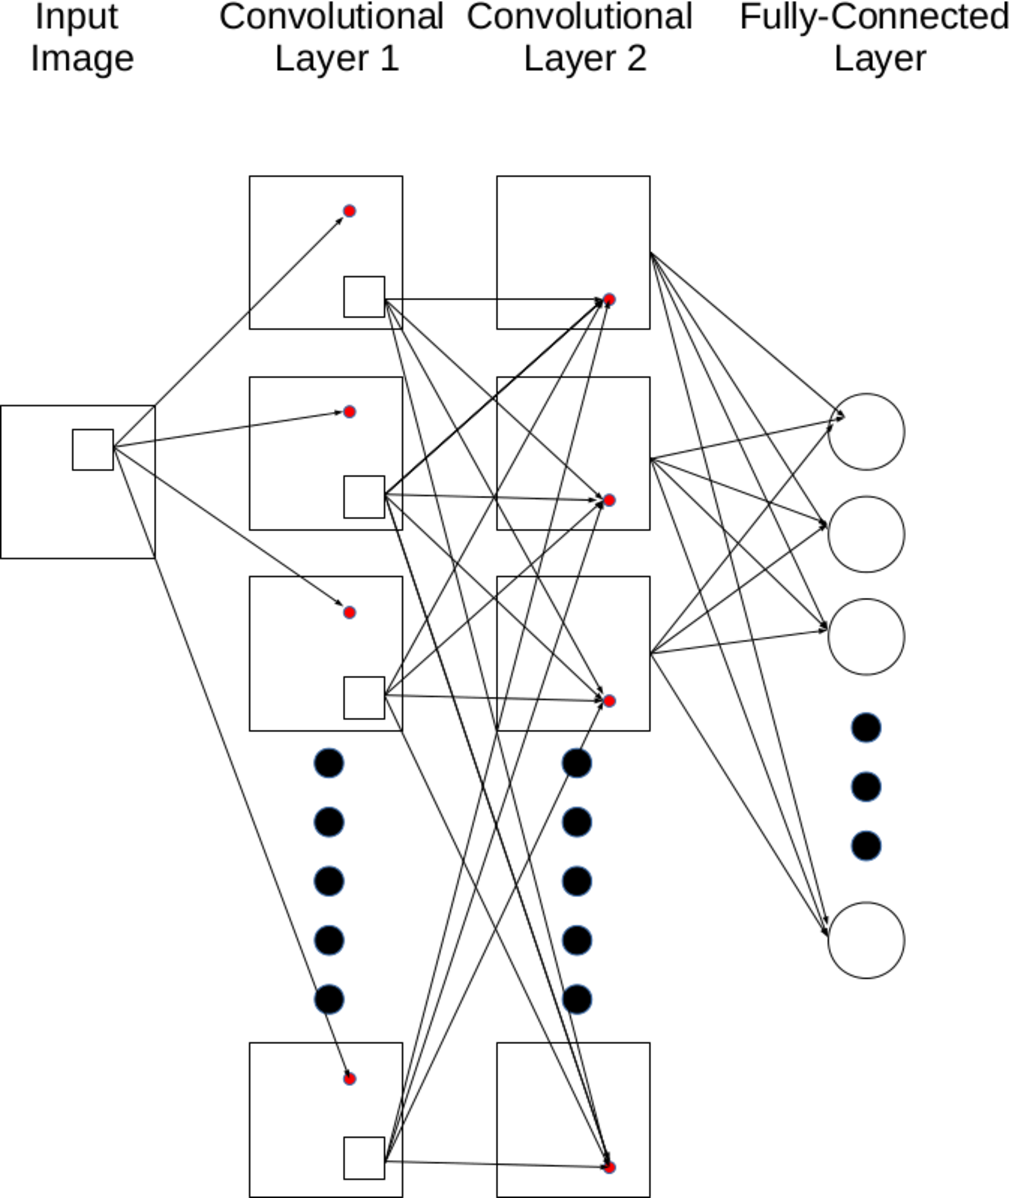
\includegraphics[width=0.6\textwidth]{Figs/Techanal/cnnarch.pdf}
      \caption{An example of a general \gls{cnn} with convolutional and fully-connected layers.}
    \label{fig:generalcnn}
\end{figure}

The activation function within a convolutional layer is another key aspect to neural networks. The activation layer is used to add non-linearity to the network and measures how well a given convolutional operation and associated bias fires for a patch in either the input image or a previous layer. Typically activation functions output between 0 and 1 to represent this measurement. In earlier adaptations of \glspl{cnn} the a sigmoid activation function was popular to map the output of a convolutional layer between 0 and 1. However, most current \glspl{cnn} take advantage of the \glspl{relu} activation function. \gls{relu} is a simple thresholding function that maps negative outputs to 0 and positive outputs are kept unchanged.
\\\\
In order to learn the parameters in a \gls{cnn} an optimisation strategy is required. The training process is to minimise a loss function in respect the inputs. Typically the learning is done through gradient descent with backpropgation. The intuition here is to update parameters after each forward iteration such that the loss calculated between input samples and their labels is decreased. Generally for each forward pass the loss is calculated as the average loss over a mini-batch of samples. This is both more efficient and produces a less stochastic learning process. Once the loss is found the gradient indicates which direction to update parameters and this information is backpropagated right through to the initial parameters.
\\\\
A key aspect of training \glspl{cnn} is how the parameters in a network are initialised. Poor initialisation of parameters can make the training process slow or impossible if the initial operations fire the activation functions too violently. Common approaches to initialisation include sampling the weights from a Gaussian distribution and setting all biases to zero. Other alternative dynamic approaches do exist, such as Xavier initialisation \cite{xavier}. In this case the architecture of the network is measured, such as number of filters in a layer, and weights are sampled according to this information. Another initialisation method is fine-tuning parameters from a pre-trained network. A pre-trained network is typically trained on a large set of data and has learnt parameters to that given task, then by updating the parameters they can be changed towards a new task. This can provide a number of benefits. Firstly, the amount of training time can be drastically reduced as strong general parameters have already been learned. Also, if the amount of training data is sparse, fine-tuning can aid such that the risk of overfitting is reduced.

%\section{Evaluation Metrics}
\section{Object Detectors}
This section will perform a technical analysis of the current primary \gls{cnn}-based object detectors.

\subsection{Faster Region-Convolutional Neural Network}
A primary \gls{cnn}-based object detector over the previous years has been Faster R-CNN \cite{fasterrcnn} and it's predecessors, Fast R-CNN \cite{fastrcnn} and R-CNN \cite{rcnn}. As mentioned in \sectionref{related}, 15 of the 21 current entries in \gls{mscoco} is Faster R-CNN based. The general method of Faster R-CNN can be split into two parts, region proposals and region classification. Region proposals aims to reduce the amount of windows that need to be tested at inference time in comparison to the previously often used sliding window approach. Rather than testing a plethora of potential object window locations, scales and aspect ratios, region proposals finds a lower number of windows that are likely to contain an object. On top of reducing the total number of testing windows, it also allows for using more expensive classification techniques such as \glspl{cnn}. There are a large number of different methods to compute region proposals, however, Faster R-CNN has one leading current methods being used in multiple other methods. The proposals are efficiently computed with a \gls{rpn}, as proposals are found directly in the network, sharing convolutional layers with the classification step. The framework of the Faster R-CNN can be seen in \figref{fasterframework}. 

\change[inline]{update faster rcnn framework figure}
\begin{figure}[H]
  \centering
    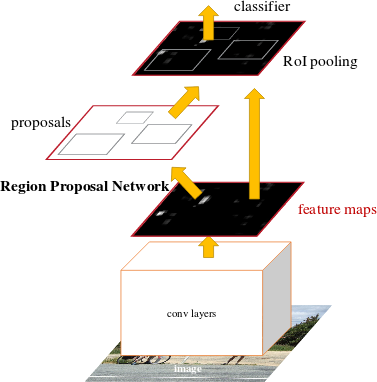
\includegraphics[width=0.6\textwidth]{Figs/Techanal/fasterframework.png}
      \caption{PLACEHOLDER. Faster R-CNN framework. A \gls{cnn} computes a feature map from which a \gls{rpn} finds region proposals. Given these proposals and the same feature map proposals are classed accordingly.}
    \label{fig:fasterframework}
\end{figure}

There a number of different possible \gls{cnn} models that can be used the compute feature maps through the convolutional layers. In the original Faster R-CNN VGG nets \cite{vgg16} were experimented with. However, since then more efficient and accurate networks have come forward, with one of the most popular being the ResNet \cite{deepres} architecture. Standard practice is to pre-train the network for classification on Imagenet followed by fine-tuning it towards object detection. Independent of the chosen network the \gls{rpn} takes as input the last feature map from the convolutional layers of the network. A small network traverses the feature map which feeds the result into two sibling fully-connected layers, a box-classification layer and a box regression layer. The box-classification layer classifies the \gls{roi} into either an object or background, with a probability being associated to each. While the latter box-regression layer attempts to fit the bounding-box to the object of interest. In order to take into account different scales and aspect ratios of objects in the feature map the \gls{rpn} uses a set of pre-defined \glspl{roi} at each sliding window location. These pre-defined \glspl{roi} are denoted as anchors. At each sliding window location a maximum of $k$ possible region proposals can be computed based upon the $k$ anchors. The anchors are user-defined into different sizes and aspect ratios. A default setting for the anchors is a total of $k$ = 9, which corresponds to 3 scales and 3 aspect ratios. The computation of the $k$ anchors at sliding window location followed by the sibling layers is visualised in \figref{rpnframework}.

\change[inline]{update rpn framework figure}
\begin{figure}[H]
  \centering
    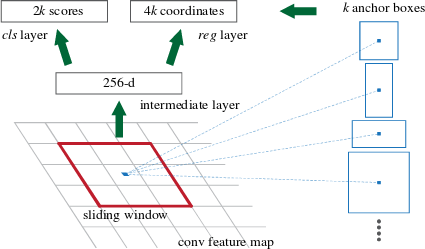
\includegraphics[width=0.6\textwidth]{Figs/Techanal/rpnframework.png}
      \caption{PLACEHOLDER. \gls{rpn} framework. The $k$ anchor boxes are placed at each sliding window location on the last feature map. The \gls{rpn} uses two sibling layers to compute the classification of object or background and perform bounding-box regression.}
    \label{fig:rpnframework}
\end{figure}

Given the set of region proposals from the \gls{rpn}, objects are classified in the $C+1$ categories based upon the same approach as in Fast R-CNN. Features are cropped for each proposal are their respective location from the same feature map given to the \gls{rpn}. Features are computed using a \gls{roi} pooling layer that uses max pooling to convert the cropped area into a pooled map of fixed spatial extent ($H \times W$), where $H$ and $W$ are hyper-parameters. In order convert each \gls{roi} into a fixed max pooled size, the \gls{roi} of size $h \times w$ is split into a grid of $H \times W$, with each sub-window being of size $h/H \times w/W$. Max pooling is then applied at each sub-window and placed accordingly in the $H \times W$ pooled layer. Following the \gls{roi} pooling layer, two fully-connected layers feed sibling layers into a classification layer and a box-regression layer, similar to those in the \gls{rpn}. However, in this instance the classification layer computes the probabilities for each of the $C+1$ classes.

\subsection{Regional Fully-Connected Network}
One of the current leading object detection methods is the \gls{rfcn} \cite{rfcn}, which as mentioned in \sectionref{related}, takes a different approach to that of the region-based methods such as Faster R-CNN. The authors of \gls{rfcn} were inspired by the recent advances in \gls{fcn} classification networks, such as ResNets, and argue that the addition of the \gls{roi}-pooling layer in the Faster R-CNN pipeline is unnatural and adds computational complexity. The authors hypothesise that the reasoning behind this addition is due to the trade-off between using a classification approach in an object detection pipeline. A defining factor in object detection is that the method should be able to respect translation variance, that translation of an object inside an object proposal should given a good indication as to how well the proposal fits the object. Whereas classification is more translation invariant, as the shifting of an object in an image does not effect how the system returns it's output. The use of the \gls{roi}-pooling layer placed in between convolutional layers means that any convolutions after this point are not translation invariant as it is not region specific. Rather than using this popular feature extractor, \gls{rfcn} uses position-sensitive score maps computed by a bank of convolutional layers. The maps add translation variance into the detection pipeline by computing scores in relation to position information with respect to the relative spatial position of an object. A \gls{roi}-pooling layer is added after the score-maps, however, no convolutional operations are done after this point ensuring translation variance.
\\\\
The overall approach of the \gls{rfcn} also consists of the popular two-stages of region proposal and region classification. Region proposal is done using the \gls{rpn} from Faster R-CNN followed by the position-sensitive score maps and \gls{roi} pooling for region classification. The overall architecture of the \gls{rfcn} can be seen in \figref{rfcnarch}.


\begin{figure}[H]
  \centering
    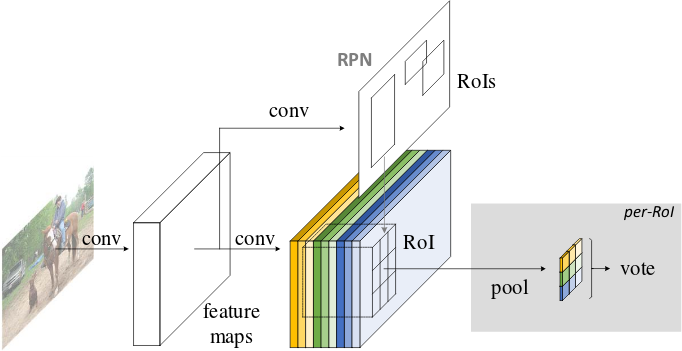
\includegraphics[width=0.8\textwidth]{Figs/Techanal/rfcnarchi.png}
      \caption{Architecture of \gls{rfcn}. Region proposals are found using the \gls{rpn} followed by classification based on a bank of position-sensitive score maps.}
    \label{fig:rfcnarch}
\end{figure}

The added translation variance post finding proposals with the \gls{rpn} is done by producing a bank of $k^2$ score maps for each object category. Therefore, there are a total of $k^2(C + 1)$ maps, where $C$ is the number of object categories plus one for a background class. The number of $k^2$ maps is due to a $k \times k$ spatial grid representing relative positions. Typically $k = 3$, therefore, the nine score maps represent position-sensitive scores for a given object category.

\change[inline]{update score maps figure}
\begin{figure}[H]
  \centering
    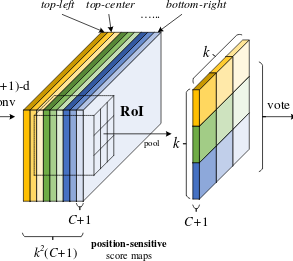
\includegraphics[width=0.4\textwidth]{Figs/Techanal/scoremaps.png}
     \caption{PLACEHOLDER. Score maps.}
    \label{fig:scoremaps}
\end{figure}

Once the bank of score maps have been computed, position-sensitive \gls{roi}-pooling is found for region classification. Each individual $k \times k$ bin pools from its corresponding location in the relevant score map. For example, the top left bin pools from that position in the top-left score map and so on. The \gls{roi}-pool is computed using average pooling for each bin which can be seen in \figref{rfcnpooling}. The final decision for a given class is determined by a vote where each of the bins are averaged, producing a $(C+1)$-dimensional vector for each \gls{roi}.

\change[inline]{update score maps figure}
\begin{figure}[H]
  \centering
    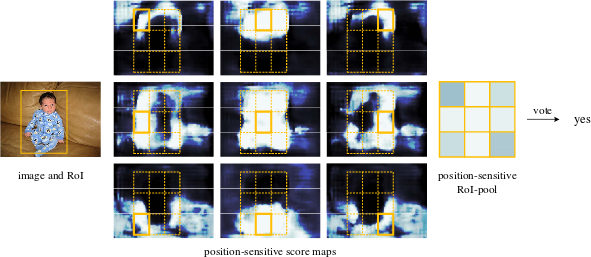
\includegraphics[width=0.6\textwidth]{Figs/Techanal/rfcnpooling.png}
      \caption{PLACEHOLDER. Position-sensitive \gls{roi}-pooling operation for a given class.}
    \label{fig:rfcnpooling}
\end{figure}

\subsection{You Only Look Once}
YOLOv2 \cite{yolov2} is one of the current best performing single shot detectors, with results on par with more commonly used object detectors while being considerably faster at test time. YOLOv2 uses a different approach than the common 2-step method of region proposal and region classification seen in Faster R-CNN and \gls{rfcn} by directly computing class probabilities on each \gls{roi}. Some of the main distinct difference between YOLOv2 and region-based methods is the use of directly predicting bounding boxes, using a modified model, and altering how the priors for anchor boxes are computed during region proposals with the \gls{rpn}. The distinct differentiator for YOLO and YOLOv2 is that bounding boxes for a given object are predicted directly rather than predicting offsets to anchors with the \gls{rpn}. This is done by splitting the image into $S \times S$ grid cells, with each cell predicting $B$ bounding boxes. Each of the $B$ boxes predict a total of 5 values: $[t_x, t_y, t_w, t_h, t_o]$. Where $t_x, t_y$ are the coordinates of the centre of the given cell. The values $t_w, t_h$ are the width and height relative to the entire image. Finally, $t_\sigma$ is the confidence of how well the predicted box fits the ground truth. The location of the bounding box is determined by these values with respect to a given cell and the offset of the cell from the top left corner of the image $(c_x, c_y)$ and the size of the anchor box is $p_w, p_h$. Then the bounding box predictions are calculated by:

\begin{equation}
\begin{split}  
  b_x = \sigma(t_x) + c_x \\
  b_y = \sigma(t_y) + c_y \\
  b_w = p_we^{t_w} \\
  b_h = p_he^{t_h}.
\end{split}
\end{equation}

Finally, the probability that the given bounding box fitting given the probability of their being an object is:

\begin{equation}  
  Pr(object) * \gls{iou}(b, object) = \sigma(t_o).  
\end{equation}

Each of the $S^2$ cells predicts $C$ conditional probabilities of it containing a given class and also being object by $Pr(Class_i \rvert Object)$. With the predicted bounding boxes and class probabilities calculated for each cell the final detections can be determined by adjusting a threshold based upon the calculation:

\begin{equation}
  Pr(Class_i \rvert Object) *  Pr(object) * \gls{iou}(b, object). 
\end{equation}

This process of using grid cells, bounding box prediction, cell class probabilities and final detections can be seen in \figref{yolomodel}.

\change[inline]{update figure}
\begin{figure}[H]
  \centering
    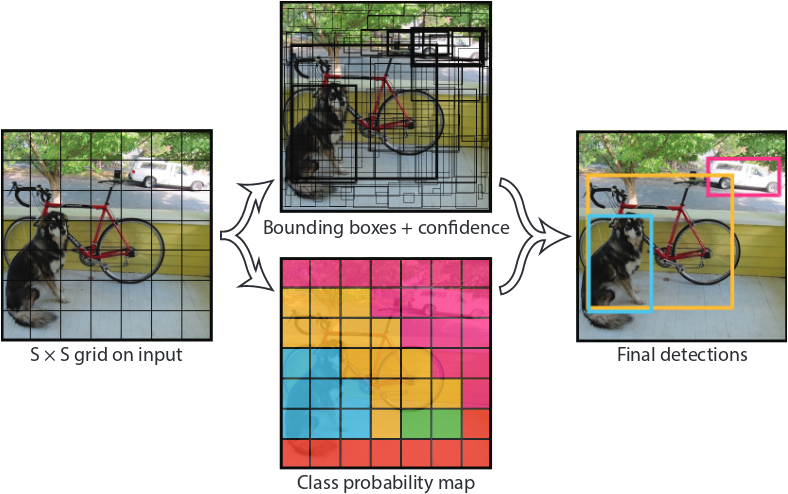
\includegraphics[width=0.8\textwidth]{Figs/Techanal/yolomodel.png}
      \caption{PLACEHOLDER. \gls{yolo} model.}
    \label{fig:yolomodel}
\end{figure}

As mentioned region proposals are found using the \gls{rpn} from Faster R-CNN \cite{fasterrcnn}. However, instead of using hand-picked priors for the anchor boxes, YOLOv2 proposed a method to learn more suitable sizes and aspect ratios. This is done by running k-means clustering on the annotated bounding boxes from the training set using a custom distance measurement. The custom measurement replaces Euclidean distance as these distances would create a bias due to more error on likely occurring on larger anchors. The custom distance measurement is designed for favourable \gls{iou} scores and is as follows:

\begin{equation}
  d(box, centroid) = 1 - IoU(box, centroid)
\end{equation}

where $box$ is the ground truth bounding box from the training set and $centroid$ is the predicted anchor box. By learning the priors YOLOv2 is able to use five anchor boxes at the same level of recall as the nine used in a typical \gls{rpn}.

YOLOv2 also goes against the grain in comparison to other state-of-the-art object detectors in regards to the choice of classification model. Rather than using the common networks such as VGG or ResNets, YOLOv2 propose their own 19 layer model dubbed Darknet-19. The model is of similar paradigm to VGG nets in that it uses mostly $3 \times 3$ convolutions and doubles the number of channels after pooling, which is also present in ResNets. But it is of considerably lower complexity than VGG-16 which consists of 15.3 billion \gls{flops}, with only 5.58 billion \gls{flops}. The baseline model has competitive results on ImageNet which can be seen in \tableref{darknetimagenet}. The baseline can be improved using standard data augmentations and also by initially training on $224 \times 224$ images followed by fine-tuning on $448 \time 448$, this is also shown as Darknet-19++ in \tableref{darknetimagenet}.

\begin{table}[h]
\centering
\caption{ImageNet classification results for the Darknet-19 model.}
\label{tab:darknetimagenet}
\begin{tabular}{|l|l|l|}
\hline
Model                                                                                       & top-1 error (\%) & top-5 error (\%) \\ \hline
Darknet-19                                                                                  & 27.1             & 8.8              \\ \hline
Darknet-19++ & 23.5             & 6.7              \\ \hline
\end{tabular}
\end{table}

To aid in the detection of small objects the Darknet-19 model is also pre-trained on high-resolution images from ImageNet prior to training for object detection. Also fine-grained features are passthrough from an earlier layer when performing prediction. This gives features from a $26 \times 26$ feature map instead of the $13 \time 13$ size at the \gls{rpn}. Finally multi-scale training is also performed.

\subsection{Benchmark Results}
\begin{comment}
	RFCN
		train data union of voc 2007 trainval and voc 2012 trainval (07+12)
		test voc 2007 test set
		conv model ResNet-101
		slightly better on voc2007 (table 3)
		slight worse than Faster+++ (winner 2015) (table4)
			more bells/whistles
			rfcn only multiscale training
				train on coco - finetune on pascal
		faster
		depth - saturated at 101

    \subsection{Object Detection with ResNets}
    ResNets generalise well to computer vision tasks other than classification, such as object detection. The winning entries in 2015 from the authors of \cite{deepres} in \gls{ilsvrc} and \gls{mscoco} challenges for ImageNet detection, ImageNet localisation, COCO detection and COCO segmentation, were based upon the faster R-CNN framework with ResNets.
\end{comment}
This section will outline the results of the aforementioned \gls{cnn}-based object detectors on leading benchmarks such as \gls{pascalvoc} and \gls{mscoco}. This includes results on the methods with different combinations of \gls{cnn} models, training data, and other bells and whistles such as multi-scale training. All results are taken from the respective authors papers.

\subsubsection{\gls{pascalvoc}}
A summary of the results on the test set of \gls{pascalvoc} 2007 can be seen in \tableref{07res}. The first column denotes which method is used while also stating the underlying \gls{cnn} model, for example VGG-16 or ResNet-101. Improvements to some of the baseline methods are also included in the first column if relevant. The improvements are online hard example mining (OHEM), multi-scale training (MSTR), multi-scale testing (MSTE), box refinement (BR), and global context (GC). Training data used in the various methods include the train set of \gls{pascalvoc} 2007 (07), train set of \gls{pascalvoc} 2012 (12), and trainval set from \gls{mscoco} (COCO). In entries when COCO is included, the detector is first trained on COCO followed by fine-tuning on 07+12. The best \gls{map} result for each combination of training data is shown in bold.


\begin{table}[h]
\centering
\caption{PASCAL VOC 2007 results.}
\label{tab:07res}
\begin{tabular}{|l|l|l|}
\hline
\textbf{method}                                                                   & \begin{tabular}[c]{@{}l@{}}\textbf{training} \\ \textbf{data}\end{tabular} & \textbf{mAP (\%)} \\ \hline
\begin{tabular}[c]{@{}l@{}}Faster R-CNN\\ VGG-16 \cite{fasterrcnn}\end{tabular}            & 07                                                       & 69.9     \\ \hline
\begin{tabular}[c]{@{}l@{}}Faster R-CNN\\ VGG-16 \cite{fasterrcnn}\end{tabular}            & 07+12                                                    & 73.2     \\ \hline
\begin{tabular}[c]{@{}l@{}}Faster R-CNN\\ ResNet-101 \cite{deepres}\end{tabular}        & 07+12                                                    & 76.4     \\ \hline
\begin{tabular}[c]{@{}l@{}}Faster R-CNN\\ ResNet-101\\ OHEM \cite{deepres}\end{tabular} & 07+12                                                    & 79.3     \\ \hline
\begin{tabular}[c]{@{}l@{}}R-FCN\\ ResNet-101 \cite{rfcn}\end{tabular}               & 07+12                                                    & 76.6     \\ \hline
\begin{tabular}[c]{@{}l@{}}R-FCN\\ ResNet-101 OHEM \cite{rfcn}\end{tabular}        & 07+12                                                    & 79.5     \\ \hline
\begin{tabular}[c]{@{}l@{}}R-FCN\\ ResNet-101 OHEM/MSTR \cite{rfcn}\end{tabular}      & 07+12                                                    & \textbf{80.5}     \\ \hline
\begin{tabular}[c]{@{}l@{}}YOLOv2 $288 \times 288$\\ DarkNet-19 \cite{yolov2}\end{tabular}                & 07+12                                                    & 69.0     \\ \hline
\begin{tabular}[c]{@{}l@{}}YOLOv2 $544 \times 544$\\ DarkNet-19 \cite{yolov2}\end{tabular}                & 07+12                                                    & 78.6     \\ \hline
\begin{tabular}[c]{@{}l@{}}Faster R-CNN\\ ResNet-101 BR/GC/MSTE \cite{deepres}\end{tabular}    & COCO+07+12                                               & \textbf{85.6}     \\ \hline
\begin{tabular}[c]{@{}l@{}}R-FCN\\ ResNet-101 OHEM/MSTR \cite{rfcn}\end{tabular}      & COCO+07+12                                               & 83.6     \\ \hline
\end{tabular}
\end{table}

A clear initial improvement is the use of ResNet-101 in comparison to the VGG-16 network, both with Faster R-CNN and \gls{rfcn}. ResNet-101 gives a \gls{map} improvement of 3.2\% in this scenario, from 73.2\% to 76.4\%. This was improvement was clear to the authors of \gls{rfcn} and therefore the only network used in their work is ResNet-101 for object detection. A small improvement of 0.2\% can also been seen for \gls{rfcn} over Faster R-CNN when using ResNet-101, both with and without \gls{ohem}. The best performing detector with 07+12 training data is \gls{rfcn} with both \gls{ohem} and MSTR (80.5\%), indicating that the addition of multi-scale training improves the result by 1\%. YOLOv2 scores slightly lower that \gls{rfcn} and Faster R-CNN. The best performing YOLOv2 network is trained to inputs of resolution $544 \times 544$, resulting in a \gls{map} of 78.6.
When using the method of training on COCO followed by fine-tuning on 07+12, Faster R-CNN with ResNet-101 and BR/GC/MSTE scoring 85.6\%. However, it is difficult to directly compare methods in this instance as the other method that uses the same training data, \gls{rfcn} with ResNet-101 and OHEM/MSTR, uses different variants of additions to the overall method. However, a general trend is that the training scheme of COCO+07+12 results in a significant improvement, with the comparable \gls{rfcn} method improving 3.1\%.

Similar results can be seen on the \gls{pascalvoc} 2012 testing set, shown in \tableref{12res}. A general standard for training on this test set is to include both the trainval and test from \gls{pascalvoc} 2007 and 2012 trainval, denoted as 07++12. As in the 2007 test set, Faster R-CNN is improved with the deeper features from ResNet-101 by 3.4\% when training with 07++12. The best result using the training set of 07++12 is with \gls{rfcn} with OHEM/MSTR, improving upon Faster R-CNN with ResNet-101 by 3.8\%. However, again it is difficult to compare due to the additions of OHEM and MSTR. The high-resolution version of YOLOv2 is again a number of percentage points behind resulting in 73.4\%. The best result is again of Faster R-CNN with ResNet-101 and BR/GC/MSTE when using COCO+07++12 as the training data with 83.8\%. \gls{rfcn} with ResNet-101 and OHEM/MSTR is similarly behind as in the 2007 test, scoring 1.8\% lower.


\begin{table}[h]
\centering
\caption{PASCAL VOC 2012 results.}
\label{tab:12res}
\begin{tabular}{|l|l|l|}
\hline
\textbf{method}                                                                  & \begin{tabular}[c]{@{}l@{}}\textbf{training} \\ \textbf{data}\end{tabular} & \textbf{mAP (\%)} \\ \hline
\begin{tabular}[c]{@{}l@{}}Faster R-CNN\\ VGG-16 \cite{fasterrcnn}\end{tabular}           & 12                                                       & 67.0     \\ \hline
\begin{tabular}[c]{@{}l@{}}Faster R-CNN\\ VGG-16 \cite{fasterrcnn}\end{tabular}           & 07++12                                                   & 70.4     \\ \hline
\begin{tabular}[c]{@{}l@{}}Faster R-CNN\\ ResNet-101 \cite{deepres}\end{tabular}       & 07++12                                                   & 73.8     \\ \hline
\begin{tabular}[c]{@{}l@{}}R-FCN\\ ResNet-101 OHEM/MSTR \cite{rfcn}\end{tabular}            & 07++12                                                   & \textbf{77.6}     \\ \hline
\begin{tabular}[c]{@{}l@{}}YOLOv2 $544 \times 544$\\ DarkNet-19 \cite{yolov2}\end{tabular} & 07++12                                                   & 73.4     \\ \hline 
\begin{tabular}[c]{@{}l@{}}Faster R-CNN\\ VGG-16 \cite{fasterrcnn}\end{tabular}           & COCO+07++12                                              & 75.9     \\ \hline
\begin{tabular}[c]{@{}l@{}}Faster R-CNN\\ ResNet-101 BR/GC/MSTE \cite{deepres}\end{tabular}       & COCO+07++12                                              & \textbf{83.8}     \\ \hline
\begin{tabular}[c]{@{}l@{}}R-FCN\\ ResNet-101 OHEM/MSTR \cite{rfcn}\end{tabular}            & COCO+07++12                                              & 82.0     \\ \hline
\end{tabular}
\end{table}

\subsubsection{\gls{mscoco}}
The final benchmark dataset to be compared is \gls{mscoco}. The results for this benchmark is more comprehensive than that shown in the \gls{pascalvoc} challenge. \gls{map} is calculated across a number of different \glspl{iou}. Also ground truths are split into three difference categories depending on the size of the object, denoted as either small, medium, or large. Training and testing data is done in two separate ways. Firstly, training is done on the train set of \gls{mscoco}, followed by testing on the validation set val. Secondly, training can be done on a combination of the aforementioned train and val (trainval), followed by testing on the test-dev set. The main results for the object detectors can be seen in \tableref{cocores}. A final testing set is also used for the YOLOv2 method, denoted trainval35k. Which is made up of the same images in trainval, however, 5,000 are removed for other validation purposes.

\begin{table}[h]
\centering
\caption{MS COCO test-dev results.}
\label{tab:cocores}
\begin{tabular}{|l|l|l|l|l|l|l|l|}
\hline
\textbf{method}                                                                 & \begin{tabular}[c]{@{}l@{}}\textbf{training}  \\ \textbf{data}\end{tabular} & \begin{tabular}[c]{@{}l@{}}\textbf{test}  \\ \textbf{data}\end{tabular} & \begin{tabular}[c]{@{}l@{}}\textbf{AP}\\ \textbf{@.5}\end{tabular} & \begin{tabular}[c]{@{}l@{}}\textbf{AP} \\ \textbf{@ [.5, .95]} \end{tabular} & \begin{tabular}[c]{@{}l@{}}\textbf{AP} \\ \textbf{small}\end{tabular} & \begin{tabular}[c]{@{}l@{}}\textbf{AP}  \\ \textbf{medium} \end{tabular} & \begin{tabular}[c]{@{}l@{}}\textbf{AP} \\ \textbf{large}\end{tabular} \\ \hline
\begin{tabular}[c]{@{}l@{}}Faster R-CNN\\ VGG-16 \cite{fasterrcnn}\end{tabular}          & train                                                    & val                                                  & 41.5                                              & 21.2                                                   & -                                                   & -                                                    & -                                                   \\ \hline
\begin{tabular}[c]{@{}l@{}}Faster R-CNN \\ ResNet-101 \cite{deepres}\end{tabular}     & train                                                    & val                                                  & 48.4                                              & 27.2                                                   & 6.6                                                 & 28.6                                                 & \textbf{45.0}                                                \\ \hline
\begin{tabular}[c]{@{}l@{}}R-FCN \\ ResNet-101 \cite{rfcn}\end{tabular}            & train                                                    & val                                                  & 48.9                                              & 27.6                                                   & \textbf{8.9}                                                 & 30.5                                                 & 42.0                                                \\ \hline
\begin{tabular}[c]{@{}l@{}}R-FCN \\ ResNet-101 \\ MSTR \cite{rfcn}\end{tabular}          & train                                                    & val                                                  & \textbf{49.1}                                              & \textbf{27.8}                                                   & 8.8                                                 & \textbf{30.8}                                                 & 42.2                                                \\ \hline
\begin{tabular}[c]{@{}l@{}}Faster R-CNN \\ VGG-16 \cite{fasterrcnn}\end{tabular}         & trainval                                                 & test-dev                                             & 42.7                                              & 21.9                                                   & -                                                   & -                                                    & -                                                   \\ \hline
\begin{tabular}[c]{@{}l@{}}Faster R-CNN \\ ResNet-101 \\ BR/GC/MSTE \cite{deepres}\end{tabular} & trainval                                                 & test-dev                                             & \textbf{55.7}                                              & \textbf{34.9}                                                   & \textbf{15.6}                                                & \textbf{38.7}                                                 & \textbf{50.9}                                                \\ \hline
\begin{tabular}[c]{@{}l@{}}R-FCN \\ ResNet-101 \cite{rfcn}\end{tabular}            & trainval                                                 & test-dev                                             & 51.5                                              & 29.2                                                   & 10.3                                                & 32.4                                                 & 43.4                                                \\ \hline
\begin{tabular}[c]{@{}l@{}}R-FCN \\ ResNet-101 \\ MSTR \cite{rfcn}\end{tabular}          & trainval                                                 & test-dev                                             & 51.9                                              & 29.9                                                   & 10.8                                                & 32.8                                                 & 45.0                                                \\ \hline
\begin{tabular}[c]{@{}l@{}}R-FCN \\ ResNet-101 \\ MSTR/MSTE \cite{rfcn}\end{tabular}         & trainval                                                 & test-dev                                             & 53.2                                              & 31.5                                                   & 14.3                                                & 35.5                                                 & 44.2                                                \\ \hline
\begin{tabular}[c]{@{}l@{}}YOLOv2\\ DarkNet-19 \cite{yolov2}\end{tabular}            & trainval35k                                              & test-dev                                             & 44.0                                              & 21.6                                                   & 5.0                                                 & 22.4                                                 & 35.5                                                \\ \hline
\end{tabular}
\end{table}

As in the \gls{pascalvoc} challenges, baseline \gls{rfcn} performs better than Faster R-CNN with ResNet-101, with \gls{ap}@.5 scoring 0.5\% and \gls{ap}@[.5, .95] 0.4\% higher. \gls{rfcn} with MSTR gives the best result when using the training set of \gls{mscoco} only. Interestingly this best result is not consistent when comparing \gls{ap} across the three object scales. For small object \gls{rfcn} with ResNet-101 is best at 8.9\%, slightly above \gls{rfcn} with ResNet-101 and MSTR (8.8\%). However, the later method is best for medium sized objects at 30.8\%, 0.3\% better than the next best method. Faster R-CNN with ResNet-101 performs best for large objects with 45.0\%, 2.8\% higher than the next best result, despite being considerably worse performing in the small and medium sized objects. When using the trainval set for training and test-dev for testing the best performing method is again Faster R-CNN with ResNet-101 and BR/GC/MSTE across all \gls{ap} modes. Again comparison is difficult as the methods do not all have the same additions to their baselines. \gls{rfcn} with ResNet-101 and MSTR/MSTE is competitive to the best result. According to the authors of the best method \cite{deepres}, the additions of box refinement gives roughly 2\% improvement, while global context gives about 1\%. This could account for the 2.5\% difference in \gls{ap}@.5. Finally YOLOv2 with DarkNet-19 performs considerably worse on \gls{mscoco}. This is especially present on smaller objects scoring 5.0\% \gls{ap}.
\begin{comment}
	previous SOTA models used in obj detect VGG 16/30 layers
	intuitively deep learning improve with more layers
		resnets proved this was not necessarily the case
		poor performance when simply stacking layers
	denoted a degradation problem
		training accuracy was poor - not all systems easy to optimise
		accuracy becomes saturated
		not overfitting, as their is higher training error - harder to optimise
	 present a new idea
	 	construction with identity mapping
	 	added layers are identity mapping - all other layers copied from learned shallower model
	 	therefore, deeper model should have no higher training error than shallower counterpart
	 	current solvers unable to do this
 	introduce deep residual learning framework
 		instead of hoping few stacked layers directly fit a desired underlying mapping
 		let layers fit residual mapping - hypothesis that this is easier to optimise
 		similar to shortcut connections - show figure and equation
 		this performs the identity mapping, no extra parameters, minimal complexity (addition)
\end{comment}

\section{Models}
\add[inline]{intro explaining backbone of models and what is covered in this section}

\subsection{VGG}
A popular model for classification and object detection tasks are the VGG nets \cite{vgg16}. At the time of their creation they displayed superior results on the \gls{ilsvrc} classification challenge in 2014, largely due to their significantly deep networks compared to previous \gls{cnn}-based approaches. The network is relatively simple, having 16 or 19 convolutional weight layers, stacked on top of each other, that only have 3$\times$3 size filters. The overall architecture of the 19 layer VGG-19 network can be seen in \figref{vggarch}. The number of channels in the convolutional layers starts at 64 and increases by a factor of 2 after each max-pooling layer to a maximum size of 512 channels. The convolutional layers have zero-padding added to preserve the spatial resolution. Therefore, the volume is only decreased by the five max-pooling layers that consist of 2$\times$2 windows at a stride of 2. After the final max-pooling layer there are a total of three fully-connected layers, two with 4096 outputs and a 1000 output layer for the case of the number of classes in \gls{ilsvrc} classification.

\begin{figure}[H]
  \centering
    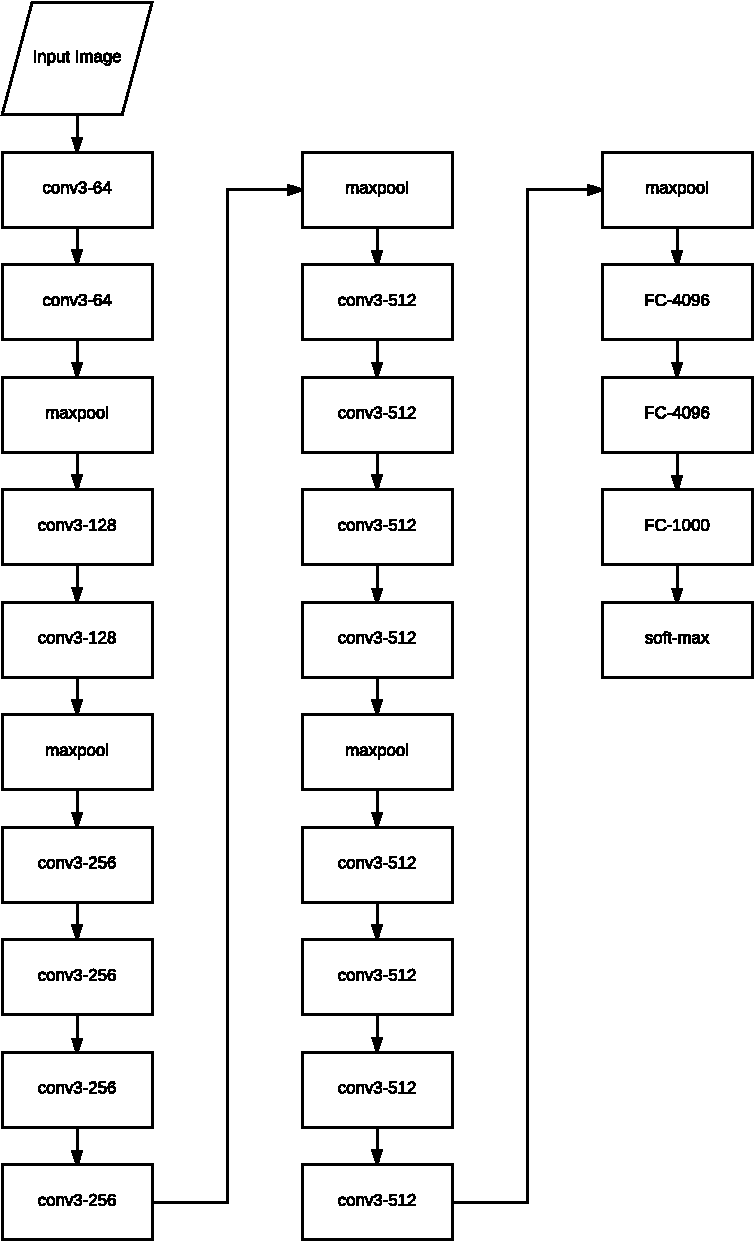
\includegraphics[width=0.5\textwidth]{Figs/Techanal/vggarch.pdf}
    \caption{General architecture of the VGG nets. In this instance the VGG-19 model is shown.}
    \label{fig:vggarch}
\end{figure}

At the time of creation, VGG nets used smaller receptive fields in comparison to other \gls{cnn} classification networks. Rather than having larger 7$\times$7 filters, VGG nets use multiple 3$\times$3 filters. An advantage to this there are more functions at a reduced relative computational cost, each with their own non-linear \glspl{relu}. Which has the effect of creating more discriminative functions \cite{vgg16}.
\\\\
As mentioned, the results on \gls{ilsvrc} classification were amongst the top performing in 2014. The entry with VGG nets took advantage of ensemble methods by averaging the softmax outputs of their top two best performing complimentary models. Additionally, the networks were trained and tested at multiple scales. Multiple crops were also taken from a given image and their softmax results averaged to give the output for each model. Using these strategies with VGG-19 models the top-1 error was 24.4\% and top-5 7.1\%. Despite these results there are a number of issues with VGG networks. Firstly, the networks are notoriously difficult to train. The aforementioned 16 and 19 layer networks were initialised using a shallower 11-layer network as convergence was so hard to achieve. Secondly, despite using smaller receptive fields the number of parameters in the networks is very large. Apart from training difficulties, this puts a large requirement on this size of GPU needed. 

\subsection{Residual Networks}
After the impressive advances of various challenges with ResNets in 2015, their use become a standard for object detection systems. With many of the entries in \gls{mscoco} and \gls{ilsvrc} being based upon ResNets. The intuition of deep neural networks is that as the model becomes deeper richer representations of the original input are found. However, as shown in the work of ResNets \cite{deepres}, it is difficult to train deeper versions of commonly used \gls{cnn} architectures. Before the appearance of ResNets one of the standard architectures were VGG nets \cite{vgg16}, consisting of 16 to 30 layers. The intuition of deeper architectures lead to better networks was explored in \cite{deepres} by stacking additional layers and creating a 56 layer \gls{cnn}. It was found that stacked deeper networks have a degradation problem and the networks converge to a testing error higher than the corresponding shallower networks. A hypothesis could be made that this is due to a deeper network overfitting the dataset, however, it was determined that this was not the case as deeper models also exhibit higher training error. The solution to this degradation problem was to to construct deeper models using identity mapping and residuals, dubbed a deep residual learning framework. With this framework a given layer learns a residual mapping between the previous layer output and operations on the output. Using this reformulation the training error in the current layer should be no greater that the previous. This core concept of a residual block is visualised in \figref{resblock}. The input $x$ is passed into the block where a mapping is computed with two weight layers with convolutional operations with a \gls{relu} operation between them, representing an alteration with $F(x)$. After this the original input (identity) is added through a shortcut connection to the mapping by $F(x) + x$. This formulation forces the convolutional layers to compute weights to learn the residual mapping $F(x)$. 

\begin{figure}[H]
  \centering
    \includegraphics[width=0.5\textwidth]{Figs/Techanal/resblock.pdf}
    \caption{Core concept of residual blocks used in ResNets.}
    \label{fig:resblock}
\end{figure}

The formulation of $F(x) + x$ requires that the dimensions of $F$ and $x$ are equal. In situations where this is not the case a linear projection $W_sx$ is performed on $x$ such that the dimensions match. The final formulation of a residual block is:

\begin{equation}
	y = F(x, {W_i} + W_sx)
\end{equation}

where $W_i$ are the weights of the convolutional layers.

In the original work, experiments on a number of different architectures with residual blocks are conducted. Firstly, ImageNet classification is evaluated using naively stacked plain networks and ResNets. The plain networks are inspired by VGG nets \cite{vgg16} with two design criteria. Firstly, for a given output feature map size the number of filters must be equal. Secondly, if the feature maps size is halved the number of filters in the layer are doubled. The ResNets are variants of these plain networks but with residual connections in each block. In order to perform a fair comparison the linear projection performed in ResNets when dimensions are altered is done with zero-padding so that no extra parameters are added. Both sets evaluated are with 18 and 34 layers. An example of plain and ResNets can be seen in \figref{plainres}.

\begin{figure}[H]
  \centering
    \includegraphics[width=0.1\textwidth]{Figs/Techanal/plainres.png}
    \caption{PLACEHOLDER. Overview of 34 layer plain and residual networks.}
    \label{fig:plainres}
\end{figure}

On top of the use of residual blocks, ResNets are also trained with scale augmentation and batch normalisation. During inference, multi-scale testing is conducted. Results on ImageNet validation top-1 error showed that the use of residual blocks aided in the optimisation of deeper architectures. \tableref{plainrestable} shows that the deeper plain networks exhibited troubles in optimisation with increased error with a deeper network. However, ResNets provided a decrease of 2.85\% between the two respective architectures.

\begin{table}[h]
\centering
\caption{Top-1 error(\%) on ImageNet validation set.}
\label{tab:plainrestable}
\begin{tabular}{|l|l|l|}
\hline
          & \textbf{plain} & \textbf{ResNet} \\ \hline
\textbf{18 layers} & 27.94 & 27.88  \\ \hline
\textbf{34 layers} & 28.54 & 25.03  \\ \hline
\end{tabular}
\end{table}

Haven shown that ResNets aid in optimisation of deep networks, the authors experimented with even deeper networks of 50, 101, and 152 layers. Due to concerns in the training time the residual blocks are altered in comparison to that shown in \figref{resblock}. The new block shown in \figref{newresblock}, $F$ consists of 3 convolutional layers of size $1 \times 1, 3 \times 3,$ and $1 \times 1$. The two sets of $1 \times 1$ layers are used to reduce complexity by reducing the input to the $3 \times 3$ layer and restoring the resulting output. 

\begin{figure}[H]
  \centering
    \includegraphics[width=0.5\textwidth]{Figs/Techanal/newresblock.pdf}
    \caption{Residual block used in deeper ResNet architectures.}
    \label{fig:newresblock}
\end{figure}


The deeper ResNets prove to give impressive results on the ImageNet validation sets as seen in \tableref{deepresimagenet}, with the very deep ResNet-152 providing the lowest error.

\begin{table}[]
\centering
\caption{Results of various deep ResNet architectures on ImageNet validation set.}
\label{tab:deepresimagenet}
\begin{tabular}{|l|l|l|}
\hline
\textbf{Method}     & \textbf{top-1 error (\%)} & \textbf{top-5 error (\%)} \\ \hline
\textbf{ResNet-34}  & 21.84            & 5.71             \\ \hline
\textbf{ResNet-50}  & 20.74            & 5.25             \\ \hline
\textbf{ResNet-101} & 19.87            & 4.60             \\ \hline
\textbf{ResNet-152} & 19.38            & 4.49             \\ \hline
\end{tabular}
\end{table}


\section{Ensemble Methods}
Ensembles of classifiers is a popular method to increase the performance of many machine learning application and problems. In object detection, most current top performing systems are ensemble based. As mentioned in \sectionref{related}, this includes the top two performing methods on \gls{mscoco} that use Faster R-CNN ensemble with variants of ResNets.
This section will give an overview of ensemble methods in machine learning, including some popular methodologies. The section is largely inspired on the concepts from the comprehensive of ensemble methods in regards to methods and applications in \cite{ensemblebook}.
\\\\
One of the main goals of ensemble systems is to reduce the variance incorporated in the training process. By reducing variance a key issue that appears in the bias-variance trade-off problem in machine learning can be addressed. Bias is the error that arises from incorrect assumptions in the learning algorithm, high bias can result in an algorithm to miss important patterns in the given problem. Whereas variance is fluctuations in the training data, if there is a high amount of variance a model can overfit to random noise. Typically systems with low bias tend to have high variance and have models that are more complicated. Therefore, in ensemble methods a goal can be to have multiple classifiers that have a similarly low bias but are different in regards to the variance in training data. By combining these models the overall variance is reduced and hence accuracy improved. An example of having different variance is to train classifiers on different subsets of the data. By doing this the assumption is that the classifiers will make different errors on a given data point, however, by combining the classifiers the errors will be cancelled out by the increased strength from lower individual variance. Each classifier is considered an ensemble member in the overall system and can have be used in one of two settings. Firstly a member can be used for classifier selection, here each classifier is trained such that it is an expert in a local part of the feature space. Then during inference one of the members are selected to answer the problem based upon a distance measurement of the data in the feature space. Alternatively the members can be weighted according to their distances to the data and combined to produce a decision. The second way in which ensemble members can be used is in classifier fusion. With this method all members are trained over the entire feature space and fused to make a composite classifier. Due to differences in training, such as ordering of training data, the individual members are slightly different and fusing them leads to lower variance.

\subsection{Building an Ensemble System}
According to \cite{ensemblebook} there are three main strategies to building an ensemble system. Namely:

\begin{enumerate}
	\item Data sampling and selection: selection of training data for individual classifiers.
	\item Training member classifiers: specific procedure used for generating ensemble members.
	\item Combining ensemble members: combination rule for obtaining ensemble decision.
\end{enumerate}

The firstly strategy aims to increase the diversity of the individual ensemble members. A common method as mentioned earlier is to train the members on different subsets of the training data. Ideally the members should not give the same output for a given data point, otherwise the ensemble is superfluous. While important that members have their individual strengths in producing correct predictions that are different, even more important is that the members produce different errors. Again, if the members produce the same errors on a data point it is not possible to reach the correct outcome. However, if members produce different errors there is the potential that individual member error can be fixed when combining outcomes. The second strategy is in regards to how the members are trained. Variability in the ensemble can be reduced by using different strategies. Third is the final step in an ensemble system, how to combine the members. This step is dependent on the type of output from the classifiers. For example, a support vector machine may only return the class label without any additional information. In this instance the popular choice is to use a majority voting strategy where labels with the highest sum is taken as the ensemble output. However, if the output of the members is continuous, such as with accompanying confidence values in neural networks, more options are present. These can include multiple arithmetic methods such as mean, average, minimum, maximum and median.



\chapter{Design}
\begin{comment}
Based upon current SOTA ensemble methods is common practice to improve generalisation of a system.
As shown in results of COCO, resolution of an object in an image a major factor in performance.
Another issue not often discussed in works is image quality. Can be a factor in performance - cite IQDNN paper
Different methods to tackle this problem. 
for resolution, dependent on two parts of the the object detector, 1. object proposals 2. classification of proposals
	if proposals have a low recall then classification part of detector is never presented with objects and no way to classify them
	if classification is poor then cannot classify.....
possible to create an ensemble for either, chosen to concentrate on the latter

plan
address pillars 1 and 3 of an ensemble system
1 - train on different subsets of data
previous works have done this randomly and tested on a validation set
here, instead actively create different subsets to train on and to test on
3 - ensemble detections of above models
majority, dynamic, etc

present method as to how to measure image quality
what is FR IQA / NR IQA?

show figure of how to ensemble

choice of ResNet-101 GPU size
\end{comment}

%\section{Design Overview}
Now that an analysis of the technical aspects of object detection with deep learning has been conducted an overview of the design of the system will be made in this section. 
Multiple choices can be made with respect to the overall architecture of the \gls{cnn}-based object detector. As covered in \sectionref{objdet}, two of the best performing systems are Faster R-CNN and R-FCN. The current core classification model used in both is the ResNet architecture. As the addition of ResNets significantly increases performance the use of these in this work is deemed crucial. However, the choice of either Faster R-CNN or R-FCN is not immediately as clear. Both methods perform similarly with respect to benchmarks such as \gls{pascalvoc} and \gls{mscoco}. But as the decision has been made to incorporate ResNets a decision on this matter was indirectly made. The GPU available in this project while being large in regards to memory is only available to train R-FCN with the ResNet-101 model. Unfortunately, due to the internal architecture of Faster R-CNN the 8GB memory on the NVIDIA GPU was not able to store all parameters while training a Faster R-CNN with ResNets. Due to the more efficient classification module in R-FCN, a ResNet backbone could be trained.
\\\\
Leading object detection systems take advantage of ensemble methods. Many of them are trained with regards to the variations in internal architecture and not specifically training experts towards solving specific challenges. Therefore, the system in this project will take advantage of the first point in \sectionref{build_ensemble}, namely data sampling and selection. The aim will be to train R-FCN with ResNet-101 on different subsets of training data with the aim to create expert ensemble members in regards robust-related challenges. Two separate factors will be chosen, one with respect to variations in the object and the other in terms of image variations. The first factor chosen is object size. As covered in \sectionref{benchresults}, in general object detection systems find it challenging to detect and classify objects with smaller resolutions. Therefore, if a system can be trained towards a subset of sizes in the training data, ideally the individual ensemble members will increase their performance on the respective sizes. The second factor chosen is image quality. As mentioned in \sectionref{qualityprob}, the quality of an image can be a factor in the overall performance of \gls{cnn}-based classification systems. Therefore members will also be trained towards subsets data split based upon this.
\\\\
Lastly, the third strategy in building an ensemble system will be addressed. Individual members predictions much be combined in an ensemble system. Therefore, approaches must be taken to combine outputs. The combination strategy is greater than only voting on which class a potential object is associated to. Bounding-boxes and the confidence of each detection is used in the calculation of metrics in both \gls{pascalvoc} and \gls{mscoco}. Therefore, these must be combined in the ensemble system as well.
\\\\
Based upon these issues the following design requirements are set with respect to the previously discussed items.

\begin{itemize}
	
	\item Object Detector Architecture.
	\begin{itemize}
		\item \gls{cnn}-based method.
		\item ResNets as backbone model.
	\end{itemize}

	\item Ensemble Data Sampling and Selection.
	\begin{itemize}
		\item Ability to measure object and image variations with respect to: 
		\begin{itemize}
			\item Object size.
			\item Image quality.
		\end{itemize}
	\end{itemize}

	\item Ensemble Training of Classifiers.
	\begin{itemize}
		\item Must be kept constant to measure effect of differing data sampling strategy.
	\end{itemize}

	\item Ensemble Combination.
	\begin{itemize}
		\item Method to combine bounding-boxes and confidences between individual ensemble members.
	\end{itemize}
\end{itemize}

Now that the general requirements have been outlined the following sections will cover the architectural considerations to ensure that the above requirements can be met.

\section{Training Ensemble Members}
The training of the R-FCN members will be done using \gls{caffe} \cite{caffe}. This was chosen due to the research being provided by the authors of R-FCN through training code and pre-trained \gls{caffe} models. However, as there is the requirement to combine detections between ensemble members, then the detections must be found based upon the same input to each model. One solution to this is to use the region proposals found using the \gls{rpn}. In a standard R-FCN the \gls{rpn} is an internal part of the network and is trained end-to-end. However, as these proposals must be constant between all ensemble members this method is not appropriate. Additionally, due to the nature of the \gls{caffe} framework, once a network has been defined and trained it is difficult to change it. For example, a standard R-FCN takes the entire image as inputs but in this work the requirement is that it takes smaller region proposals. The solution to these points is to train the networks using a method inspired by the 4-step alternating training method presented by the Faster R-CNN authors \cite{fasterrcnn}. The process can be seen in \figref{4steptrain}.

 \begin{figure}[H]
  \centering
    \includegraphics[width=1.0\textwidth]{Figs/Design/4steptrain1.pdf}
      \caption{Flow chart showing the alternating training method.}
    \label{fig:4steptrain}
\end{figure}

In this approach the overall network in trained in multiple steps rather than an end-to-end method. In the first step, an \gls{rpn} is trained to determine region proposals, the \gls{rpn} is initialised from a pre-trained ImageNet model and fine-tuned to the proposal task. Next a \gls{rfcn} is trained based upon the proposals found in the previous step. This network is also initialised with a pre-trained ImageNet model. In step three, another \gls{rpn} is trained but initialised using the \gls{rfcn} from step two. In this step the convolutional layers that are shared between the \gls{rfcn} and \gls{rpn} are fixed and only the layers unique to the \gls{rpn} are updated. By training a model with this approach a testing image is able to run through the same steps as a \gls{rfcn} trained end-to-end, however, as the networks are split into different models it is also possible to use the stages of the method individually. Creating a solution for finding region proposals with an external \gls{rpn} and having a \gls{rfcn} that can take the proposals as inputs. 
\\\\
An additional benefit to training \glspl{rfcn} in this manner is that once a baseline model has been created only one part needs to be re-trained. As the aim is to train various ensemble members to different subsets of data only the \gls{rfcn} in stage 2 is required to be re-purposed. The \gls{rpn} in stage 3 should be kept constant based on the baseline model as it will provide the shared proposals for test images. Therefore, once a systematic approach has been found for splitting data for both train and test based on the data sampling and selection requirements the detection part of the \gls{rfcn} can be trained towards its expert area. The following sections will explain how the subsets of data will be selected.

\subsection{Object Size Data Sampling}
The area of a region proposal found with a \gls{rpn} gives an indication as to the approximate size of a potential objects. Therefore, the area for all proposals on the training set can be computed from the output of the second step in stage 2 shown in \figref{4steptrain}. Once the area of all proposals are computed an appropriate split of the data can be determined depending on the area distribution. The main requirement in creating the subsets of data is that equal number of ground truth samples should be present in both.

\subsection{Image Quality Data Sampling}
There are many choices for computing the quality of an image. A popular area of research for this purpose is \gls{iqa}. These methods aim to determine the subjective quality of an image. There are two forms of \gls{iqa}, \gls{friqa} and \gls{nriqa}. \gls{friqa} approaches require the original, undistorted reference image in order to determine quality. Whereas, \gls{nriqa} do not have this information available \cite{deepiqa}. As the aim is to determine the level of image quality on one of the benchmark datasets, no reference image is present. Therefore, an \gls{nriqa} method is required. Current state-of-the-art within \gls{nriqa} is also deep learning based and works are typically trained on \gls{iqa} datasets. Datasets include \gls{live} dataset \cite{livepaper} \cite{liveweb}, TID2013 \cite{tid2013} and CSIQ \cite{csiq}. The datasets consist of source reference image and have artificially created counterparts with varying levels of distortion. Distortions include, such as in the LIVE dataset, JPEG2000 compression, JPEG compression, additive white Gaussian noise, Gaussian blur and bit errors from a fast fading Rayleigh channel. Models can then be trained to predict subjective quality based on ground truth user determined quality measurement.
\\\\
Based upon this, an \gls{nriqa} method can be used to determine the level of image quality with respect to a number of different distortions. Then as in object size training, if possible, the data will be split into different training subsets. A leading \gls{cnn}-based \gls{nriqa} method will be used and the specific network and implementation details will be covered in \sectionref{iqaimp}.

\subsection{\gls{rfcn} Training}
Training of the baseline \gls{rfcn} model shown in \figref{4steptrain} is done using \gls{sgd} optimisation with largely the same parameters across the five different training parts. The parameters are adapted from \cite{rfcn} and can be seen in \tableref{trainparams}. All models start with a base learning rate of 0.001 which is dropped by a factor of 0.1 once in the process. This is done after 80,000 iterations for the \gls{rfcn} models and after 60,000 for the \glspl{rpn}. The learning rate is controlled with a momentum of 0.9 and weight decay of 0.0005. The two \gls{rfcn} models are trained for 120,000 iterations, while the three \glspl{rpn} are trained for 80,000.

\begin{table}[h]
\centering
\caption{Common \gls{sgd} optimisation parameters for the 5 training parts of the baseline \gls{rfcn} model.}
\label{tab:trainparams}
\begin{tabular}{|l|l|}
\hline
\textbf{Parameter}            & \textbf{Value}  \\ \hline
Base learning rate   & 0.001  \\ \hline
Learning rate policy & step   \\ \hline
Gamma                & 0.1    \\ \hline
Momentum             & 0.9    \\ \hline
Weight decay         & 0.0005 \\ \hline
\end{tabular}
\end{table}

 Both networks are trained with a batchsize of one example per iteration. In the \gls{rpn} models the batches are simply one ground truth example per iteration. Whereas, the training of the \glspl{rfcn} sample 128 mini-batches from a given image. These mini-batches can consist of both object class samples and background samples. 
 The only data augmentation used in training is horizontal flipping of images, effectively creating double the amount of training examples.

 \subsection{Object Detection Benchmark Choice}




\chapter{Implementation}
\begin{comment}
	Split data according to percentile
	RFCN resnet-101
	Pascal voc heavily skewed to smaller objects. Show plot
	50th percentile 13892.0
		test data also split according to this value
		cannot simply do by image basis - some images have multiple objects GTs - show figure
			total of 12275 GTs when doing this, still 3384 that are larger
		test images if only small images present - 697 images, 


	Results
		RFCN ResNet-101: 0.7632
		Model - 07++12 < 50th percentile
			All data: 0.5960


    %%%%%%%%%%%%%%%%%%%%%%%%%%%% RFCN 5 Stage Split%%%%%%%%%%%%%%%%%%%%%%%%%
    Train networks with object proposals from an RPN network
        many more object proposals than using GTs - 9,979,342 vs 80,116
            split also different due to this - skew towards smaller objects
                Median of GTs - 19,205.5 vs RPN GTs - 4,864.0
    Objective is to split data into equally size. What is more correct? Equal size based on true GTs or on RPNs
        if based on GT median - Small - 6,410,914 (64.25\%) vs Large - 3,598,428 (35.75\%)
        if based on RPN median - Both - 4,989,671 (50/50)
    However, test may not be equally as split
        Test proposals for network - Total - 1,418,317
            Split on GT - Small - 790,607 (55.74\%) Large -  627,710 (44.25\%)
            Split on RPN - Small - 540,767 (38.0\%) Large - 877,550 (61.87\%)

    RPN GT Training
        RPN proposals is much larger than training with only GTs
            using only GTs 80,116 vs 9,989,342
                due to proposals finding many more examples
            however, still only the correct amount of GTs labels. eg. GT = 3, background = 300
        therefore, when splitting important that one of the splits does not have significantly less GT examples.
        if split by GT median (19,205.5)
            equal number of GT training examples - 40,058 - fits well with GT
            background examples - Small - 3,528,370 vs Large - 6,370,859
        if split by all median
            skew towards larger objects
            Small - 19,992 vs Large - 60,116
            Background  - Small - 4,929,297 vs Large - 4,969,369


\end{comment}

\section{Resolution-Aware Object Detection}
Object detectors are commonly more accurate on objects that cover a larger number of pixels in an image. This is intuitive as objects with a lower resolution objectively have less details that can describe them. The poorer performance can be seen in \tableref{cocores}, for all object detectors the \gls{ap} is considerably lower for smaller objects in comparison to both medium and large. The best performing detector from \cite{deepres}, has an \gls{ap} difference of 35.3\%, from 50.9\% for large objects to 15.6\% for small. 
A potential method of tackling this issue is to train multiple detectors on separate partitions of the training data according to the size of the object. While deep-based \gls{cnn} have millions of parameters to generalise from training to testing, the difference between small and large objects may skew the learning towards the latter. In order to test this hypothesis an initial test will be conducted on the \gls{pascalvoc} dataset. However, \gls{pascalvoc} does not have the same definition of objects sizes as in \gls{mscoco}. Therefore, the distribution of the bounding boxes from the training set must be analysed in order to determine an appropriate split of data based on object size. This was done by parsing all of the bounding box coordinates in the 07++12 training set and calculating the area. A histogram of the area can be seen in \figref{0712hist}. There is a clear tendency to smaller objects in the training set with a clear skew towards the left of the figure.

\begin{figure}[H]
  \centering
    \includegraphics[width=0.6\textwidth]{Figs/Implementation/0712hist.pdf}
      \caption{Histogram of the \gls{pascalvoc} 07++12 bounding box area.}
    \label{fig:0712hist}
\end{figure}

As there is no clear way to split the data into three sets with equal amounts of data, the split was instead done into into two sets, one for small objects and another for larger. The split was made at the median bounding box area which is 13,892 pixels. Therefore, the dataset with bounding box area less than 13,982 pixels is denoted 07++12$_{small}$ and objects larger make up the dataset 07++12$_{larger}$.

Identical \gls{rfcn} with ResNet-101 networks were trained on either sets of data. Additionally the exact same training strategies were used in both instances which are outlined in \tableref{resawareparams}.

\begin{table}[h]
\centering
\caption{Learning parameters for the set of resolution-aware \gls{rfcn} object detectors.}
\label{tab:resawareparams}
\begin{tabular}{|l|l|}
\hline
\textbf{Parameter}            & \textbf{Value}  \\ \hline
base learning rate   & 0.001  \\ \hline
learning rate policy & step   \\ \hline
gamma                & 0.1    \\ \hline
stepsize             & 80,000 \\ \hline
momentum             & 0.9    \\ \hline
weight decay         & 0.0005 \\ \hline
\end{tabular}
\end{table}

Testing was done on the 07 test set but also split according to the median threshold found in the training data. The two testing sets are denoted as 07Test$_{small}$ and 07Test$_{larger}$. The size of the two test sets are 7,827 and 7,149 ground truth bounding boxes respectively. Histogram for the sets can be seen in \figref{smalltesthist} and \figref{largetesthist}.


\begin{figure}[H]
    \centering
    \begin{subfigure}[b]{0.45\textwidth}
        \center
        \includegraphics[width=\textwidth]{Figs/Implementation/testsmallhist.pdf}
        \caption{}\label{fig:smalltesthist}
    \end{subfigure}
    \begin{subfigure}[b]{0.45\textwidth}
        \center
        \includegraphics[width=\textwidth]{Figs/Implementation/testlargehist.pdf}
        \caption{}\label{fig:largetesthist}
    \end{subfigure}
    \caption{}
    \label{}
\end{figure} 

The results for the object detectors trained on the separate partitions of training data and a the baseline detector trained on all the data against the three sets of tests can be seen in \tableref{resresults}. The table shows that the detectors trained on the same relative size of data perform best. In the instance of 07Test$_{small}$, its counterpart 07++12$_{small}$ gives a result 04 0.34 \gls{map}. This is an improvement of 12\% in comparison to the model trained on all of the data (07++12) which has a \gls{map} of 22.16\%; a relative improvement of 35\%. The model trained on the data of larger objects, 07++12$_{larger}$, is very poor at detecting smaller objects scoring 3.08\%. In this case of 07Test$_{larger}$, the model trained on 07++12$_{larger}$ data is the best performing at 76.60\%. A similar improvement is \gls{map} is present in this instance in comparison to the model trained on all of the data. Overall there is an increase of 12.36\%, which is a relative improvement of 16\%. Finally, the best performing on all of the 07 test data is the model trained on 07++12.


\begin{table}[h]
\centering
\caption{Results}
\label{tab:resresults}
\begin{tabular}{|l|l|l|}
\hline
\textbf{Train Data}    & \textbf{Test Data}     & \textbf{mAP (\%)} \\ \hline
07++12$_{small}$ & 07Test$_{small}$  & \textbf{34.10}   \\ \hline
07++12$_{larger}$  & 07Test$_{small}$ & 3.08     \\ \hline
07++12   & 07Test$_{small}$           & 22.16    \\ \hline
07++12$_{small}$ & 07Test$_{larger}$  &  36.40   \\ \hline
07++12$_{larger}$ & 07Test$_{larger}$ &  \textbf{76.60}   \\ \hline
07++12 & 07Test$_{larger}$           &  64.34   \\ \hline
07++12$_{small}$       & 07   & 62.65    \\ \hline
07++12$_{larger}$       & 07  &  59.65   \\ \hline
07++12        & 07            &  \textbf{76.35}   \\ \hline 
\end{tabular}
\end{table}


\change[inline]{update following explanation}
Ensemble of above networks proved not to be possible due to Caffe network architecture. Once networks have been trained as an end-to-end method, the networks were not able to take object proposals as inputs. Solution instead to train the network in 5 stages. Much slower. Result on VOC2007: 79.59 vs end to end: 76.35 

While \tableref{resresults} shows that it is possible for a \gls{rfcn} network to be optimised to objects of a certain size, a more powerful approach is to combine the two networks in an ensemble during testing. Given a potential object, the ensemble should weight one of the networks outputs accordingly. A simple example in this case would be to weight one of the outputs by 100\%, if the potential object is below or above the threshold found in the training data. The results gathered in \tableref{resresults} are much more naive than this, simply splitting the testing data and only using one trained network at a time. Object proposals will needed to be known during inference to ensure that the outputs of the networks in an ensemble are performing classification in the same locations. On top of this, new networks will needed to be trained on subsets of smaller and larger data due to the internal architecture of \gls{caffe} networks. The networks in the ensemble will need to take object proposals as inputs, however, the above mentioned networks are trained based upon the end-to-end versions of the \gls{rfcn}. These do not take proposals as inputs but rather have an internal \gls{rpn}. Therefore, the new networks are trained using 4-step alternating training used in the original Faster R-CNN paper \cite{fasterrcnn}. In this approach the overall network in trained in multiple steps rather than an end-to-end method. In step one a \gls{rpn} is trained to determine region proposals, the \gls{rpn} is initialised from a pre-trained ImageNet model and fine-tuned to the proposal task. Next a \gls{rfcn} is trained based upon the proposals found in the previous step. This network is also initialised with a pre-trained ImageNet model. In step three, another \gls{rpn} is trained but initialised using the \gls{rfcn} from step two. In this step the convolutional layers that are shared between the \gls{rfcn} and \gls{rpn} are fixed and only the layers unique to the \gls{rpn} are updated. In this final step, the shared layers between the two networks are again kept fixed and the layers unique to the \gls{rfcn} are updated. By training a model with this approach a testing image is able to run through the same steps as a \gls{rfcn} trained end-to-end, however, as the networks are split into different models it is also possible to use the stages of the method individually. Creating a solution for finding region proposals with an \gls{rpn} and having a \gls{rfcn} that can take the proposals as inputs. 
\\\\
A potential shortcoming of using \gls{rpn} proposals as inputs to training a \gls{rfcn} rather than using ground truth bounding boxes is that a \gls{rpn} likely finds many more examples of objects that actually exist in an image. For a given image, an \gls{rpn} may find hundreds of potential objects despite an image only containing a couple of true positive examples. This can be solved by setting the proposals with the highest confidence as the ground truth examples and labelling the remaining proposals as the background class. This is a stark comparison to the end-to-end training approach as there are now many more training examples and a large skew towards the background class. Whereas the end-to-end approach does not train on any background examples. With this approach, the total number of training examples is increased from 80,116 to 9,979,345. This large increase in training examples also poses a question on how to split the \gls{rpn} proposals such that two networks can be trained towards small and large objects respectively.

\section{Image Quality Assessment}\label{sec:iqaimp}
To evaluate the amount of distortions in the dataset a method for \gls{iqa} is needed. A recent state of the art method is that of deep IQA \cite{deepiqa}. Deep IQA is a \gls{cnn}-based \gls{nr} \gls{iqa} method that can be trained to measure the subjective visual quality of an image. It is deeper than previous \gls{cnn}-based \gls{iqa} methods with the architecture being inspired by VGG nets \cite{vgg16}. Deep IQA consists of 14 convolutional layers, 5 max-pooling layers and 2 fully-connected layers. The architecture is shown in \figref{deepiqa_arch}. The convolutional layers are all 3$\times$3 convolution kernels and activated using \gls{relu}. Inputs to each convolutional layer are zero-padded to ensure output size is equal to the input. Max-pooling layers consist of 2 $\times$ 2 sized kernels. The network is trained on mini-batches of 32 $\times$ 32 patches. During inference non-overlapping patches are sampled from the image and image quality scores are predicted for each instance. The patch scores are averaged for the final score for the entire image. 

\begin{figure}[H]
  \centering
    \includegraphics[width=0.3\textwidth]{Figs/Implementation/deepiqa_arch.pdf}
      \caption{Architecture of the deep IQA network. Notation for convolutional layers are conv(receptive field size)-(number of channels) and fully-connected layers are FC(number of channels).}
    \label{fig:deepiqa_arch}
\end{figure}

Training deep IQA requires a database of annotated images with both reference images and distorted counterparts. The following section will outline the database used in this project for \gls{iqa} training.

\subsection{LIVE Image Quality Database}
Deep IQA assesses three different datasets for this purpose. These are \gls{live} which consists of 5 different distortions \cite{livepaper}, TID2013 \cite{tid2013} with 24 different distortions and CSIQ \cite{csiq} with 5 types. For simplicity purposes the only \gls{live} dataset is chosen for this project. The dataset was made for the purposes of evaluating the subjective visual quality of images in regards to the five distortion types. The distortions are generated from 29 colour reference images that are of both high-resolution and high quality. An example of images from the dataset can be seen in \figref{live_ex}. The references image were collected to have a wide variety in different content, this includes faces, people, animals, nature and man-made objects.

\begin{figure}[H]
    \centering
    \begin{subfigure}[b]{0.4\textwidth}
        \center
        \includegraphics[width=\textwidth]{Figs/Implementation/bikes.pdf}
        \caption{}\label{fig:}
    \end{subfigure}
    \begin{subfigure}[b]{0.4\textwidth}
        \center
        \includegraphics[width=\textwidth]{Figs/Implementation/buildings.pdf}
        \caption{}\label{fig:}
    \end{subfigure}
    \begin{subfigure}[b]{0.4\textwidth}
        \center
        \includegraphics[width=\textwidth]{Figs/Implementation/monarch.pdf}
        \caption{}\label{fig:}
    \end{subfigure}
    \begin{subfigure}[b]{0.4\textwidth}
	    \center
	    \includegraphics[width=\textwidth]{Figs/Implementation/paintedhouse.pdf}
	    \caption{}\label{fig:}
    \end{subfigure}
    \caption{Examples of reference images from the \gls{live} dataset.}
    \label{fig:live_ex}
\end{figure} 

The five distortions generated from the reference images are Gaussian blur, white noise, JPEG compression, JPEG2K compression and fast fading. By varying the parameters used in creation of the distortions a larger database is created for each type. The total number of images is 982 where 174 are for Gaussian blur, white noise and fast fading. JPEG and JP2K compression have 233 and 227 images respectively. The distorted images were created as follows:

\begin{itemize}
	\item Gaussian blur: blur is added to the images using a circular-symmetric Gaussian kernel of standard deviation $\sigma_B$. The values of $\sigma_b$ are sampled between the range of 0.42 to 15 pixels.
	\item White noise: Gaussian white noise of standard deviation $\sigma_N$ is added to all RGB pixels. Firstly, pixel values are scaled to between 0 and 1. $\sigma_N$ varying between 0.012 and 2.0 is added, afterwards pixel values are rescaled back between 0 and 255.
	\item JPEG compression: compression artefacts are added to the reference bitmap images with JPEG at bit rates between 0.15 \gls{bpp} to 3.34 \gls{bpp}.
	\item JP2K compression: artefacts added ranging between 0.028 \gls{bpp} to 3.15 \gls{bpp}.
	\item Fast fading: this distortion represents errors that can occur when a JP2K bitstream is transmitted over a wireless channel. The receiver signal-to-noise-ratio is varied between 15.5 to 26.1dB for bit errors.
\end{itemize}

Subjective image quality values were calculated by showing human subjects all images, including reference images, and asking them to rate the image as either bad, poor, fair, good, or excellent. The rating was done using a slider on a graphical interface with the five possibilities being evenly spaced. A value between [1, 100] was then found depending on where the subject paced their rating. \gls{dmos} were calculated for each image and averaged between all users for the final image quality annotation for an image. A low \gls{dmos} represents high image quality and a high \gls{dmos} is a low quality image. \figref{gb_ex} shows an example of an image with four varying levels of Gaussian blur and their \gls{dmos} values.

\begin{figure}[H]
    \centering
    \begin{subfigure}[b]{0.4\textwidth}
        \center
        \includegraphics[width=\textwidth]{Figs/Implementation/img173.pdf}
        \caption{\gls{dmos}: 0.0}\label{fig:}
    \end{subfigure}
    \begin{subfigure}[b]{0.4\textwidth}
        \center
        \includegraphics[width=\textwidth]{Figs/Implementation/img96.pdf}
        \caption{\gls{dmos}: 23.24}\label{fig:}
    \end{subfigure}
    \begin{subfigure}[b]{0.4\textwidth}
        \center
        \includegraphics[width=\textwidth]{Figs/Implementation/img103.pdf}
        \caption{\gls{dmos}: 40.40}\label{fig:}
    \end{subfigure}
    \begin{subfigure}[b]{0.4\textwidth}
	    \center
	    \includegraphics[width=\textwidth]{Figs/Implementation/img11.pdf}
	    \caption{\gls{dmos}: 75.92}\label{fig:}
    \end{subfigure}
    \caption{Four example images from the Gaussian blur distortion set. Respective \gls{dmos} scores are shown on the image and below.}
    \label{fig:gb_ex}
\end{figure} 

Given the annotated \gls{dmos} values a system can be trained to predict the image quality of an image. The following section will outline how to train deep IQA for this purpose.

\subsection{Training Deep IQA}
In the original work the deep IQA model \cite{deepiqa} is trained for all five distortion types present in \gls{live} \cite{livepaper} \cite{liveweb}. While this can provide insights into general image quality, individual models are needed to create a potentially more powerful ensemble. The \gls{nriqa} model was provided by the authors and by taking advantage of the fine-tuning technique, models for each of the individual distortions can be trained in a timely manner. The model was provided for the Chainer framework \cite{chainer} and fine-tuning of individual models were done using this. Fine-tuning takes a previously trained model and uses these parameters as a starting point, rather than other commonly used initialisation techniques such as using a Gaussian distribution. As the model is already trained towards all distortions the assumption can be made that only a shorter training cycle is necessary to the new task. The five fine-tuned models are trained in a similar manner to that of the provided model following the guidelines in the original work \cite{deepiqa}. 
\\\\
In the \gls{live} dataset there are 29 reference images from where the respective distortions have been created. When training deep IQA, the reference images are randomly split into 17 training images, 6 validation images and 6 test images. The deep IQA models are trained using mini-batches consisting of a total of 128 patches per forward/backward pass. The patches are sampled from four randomly selected images from the training split and each image accounts for 32 of the 128 patches in the mini-batch. This process is continued until no more patches are available for mini-batch sampling. This constitutes a completed epoch and all patches are again available for the next epoch. The model provided by the authors was trained for 3,000 epochs, however, as mentioned fine-tuning can drastically reduce the number of epochs required. Therefore, the models for the five distortions are trained for only 500 epochs each. The optimisation method for parameter updates is Adam \cite{adam}. The optimisation settings for Adam are unchanged to that of those used in training the original model. They are as $\beta_1$ = 0.9, $\beta_2$ = 0.999, $\epsilon$ = 10$^{-8}$ and $\alpha$ = 10$^{-4}$. A total of 10 models are trained for each distortion type, each on their individual random split of the 29 reference images. After each of the 500 epochs the model is evaluated on the validation set and the epoch with the best performance is chosen as the final model for testing. The evaluation metrics used for both the validation and test set is \gls{lcc} and \gls{srocc}. \gls{lcc} is used for prediction accuracy as it is a measure of the linear correlation between two sets of data. \gls{srocc} evaluates the prediction monotonicity by measuring the rank correlation between the two sets. For both metrics a value of +1 indicates a positive correlation, 0 is no correlation, and -1 is a negative correlation.
\\\\
The mean results for each of the distortion types from their 10 models can be seen in \tableref{iqaavg}. Each best performing model on the respective validation sets are run on the testing sets and averaged. The results showed that well-performing deep IQA models were successfully trained towards the individual distortion types. The following section will cover how the \gls{pascalvoc} data will be split in subsets based upon these deep IQA models.

\begin{table}[h]
\centering
\caption{Average results from 10 trained deep IQA models for each distortion type.}
\label{tab:iqaavg}
\begin{tabular}{|l|l|l|}
\hline
\textbf{Distortion Type} & \textbf{\gls{lcc}}    & \textbf{\gls{srocc}}  \\ \hline
Gaussian Blur   & 0.9750 & 0.9681 \\ \hline
White Noise     & 0.9957 & 0.9887 \\ \hline
JPEG            & 0.9805 & 0.9523 \\ \hline
JP2K            & 0.9788 & 0.9600 \\ \hline
FF     & 0.9679 & 0.9505 \\ \hline
\end{tabular}
\end{table}


\subsection{PASCAL VOC Data Split}
Each model for the five distortion types and run through the 07+12 dataset in order to give an indication to the respective distributions, as done for the object sizes in \sectionref{resawareSec}. The distributions can been seen in the histograms in \figref{iqdist}.

\begin{figure}[H]
    \centering
    \begin{subfigure}[b]{0.4\textwidth}
        \center
        \includegraphics[width=\textwidth]{Figs/Implementation/WhiteNoisedistred.pdf}
        \caption{}\label{fig:dist_wn}
    \end{subfigure}
    \begin{subfigure}[b]{0.4\textwidth}
        \center
        \includegraphics[width=\textwidth]{Figs/Implementation/GaussianBlurdistred.pdf}
        \caption{}\label{fig:dist_gb}
    \end{subfigure}
    \begin{subfigure}[b]{0.4\textwidth}
        \center
        \includegraphics[width=\textwidth]{Figs/Implementation/JPEGCompressiondistred.pdf}
        \caption{}\label{fig:dist_jp}
    \end{subfigure}
    \begin{subfigure}[b]{0.4\textwidth}
        \center
        \includegraphics[width=\textwidth]{Figs/Implementation/JP2KCompressiondistred.pdf}
        \caption{}\label{fig:dist_jk}
    \end{subfigure}
  	\begin{subfigure}[b]{0.4\textwidth}
        \center
        \includegraphics[width=\textwidth]{Figs/Implementation/FastFadingdistred.pdf}
        \caption{}\label{fig:dist_ff}
    \end{subfigure}
    \caption{Histograms representing the distribution of image quality for the five distortions trained from the \gls{live} image quality dataset. The distortions shown are white noise (a), Gaussian blur (b), JPEG compression (c), JP2k compression (d), fast fading (e).}
    \label{fig:iqdist}
\end{figure} 

The distribution for white noise and Gaussian blur is skewed towards a higher image quality as seen in \figref{dist_wn} and \figref{dist_gb} and also to a lesser extent in fast fading in \figref{dist_ff}. Whereas the image quality for compression distortions is somewhat of a Gaussian nature in \figref{dist_jp} and \figref{dist_jk}. For determining an appropriate manner to split the data the same constraints are made as in that for object sizes, namely that both subsets of data should have an equal number of ground truths to train on. Again by taking the median for each of the five distributions can satisfy this. The respective medians can be seen in \tableref{iq_splits}.

\begin{table}[h]
\centering
\caption{Threshold values used for each distortion type to create even subsets of training data from 07+12.}
\label{tab:iq_splits}
\begin{tabular}{|l|l|}
\hline
\textbf{Distortion Type}   & \textbf{Median} \\ \hline
White Noise       & 0.599  \\ \hline
Gaussian Blur     & 5.607  \\ \hline
JPEG Compression  & 15.660 \\ \hline
JP2K Compression & 11.747 \\ \hline
Fast Fading       & 13.373 \\ \hline
\end{tabular}
\end{table}

A skewed distribution of data was also present for object sizes, however, creating two subsets of data for high and low white noise image quality does not appear to be feasible. The combination of both the heavy skew and half of the data lying below 0.599 indicates that a minimal amount of white noise distortion is present in the 07+12 dataset. Therefore, this distortion is not considered for part of the ensemble. While the Gaussian blur image quality is also skewed it is similar to that of the the object sizes and therefore is deemed appropriate to split based upon its median of 5.607. The remaining distributions are much less skewed and a total of eight R-FCN models will be trained for the high and low levels of image quality for the distortions Gaussian blur, JPEG compression, JP2K compression and fast fading. Therefore, in total there will be ten R-FCN models trained including the two for smaller and larger object sizes.
\\\\
The 07+12 dataset has a total of 16,551 images and as this data is to be distributed into eight different subsets there is a possibility that there is a high level of overlap between the sets. As the aim of the ensemble is to learn to detect objects based upon different information, if subsets are two similar there may be potentially no advantage gained between two or more models. Therefore, a comparison matrix is used to evaluate how much the different combinations of 07+12 match. This can be seen for higher quality subsets in \tableref{highcomp}, lower quality in \tableref{lowcomp} and between lower and higher quality in \tableref{lowhighcomp}.

\begin{table}[h]
\centering
\caption{Comparison matrix for the percentage of matching data for image quality data for higher quality.}
\label{tab:highcomp}
\begin{tabular}{|l|l|l|l|l|}
\hline
             & \textbf{Gaussian Blur}  & \textbf{JPEG} & \textbf{JP2K} & \textbf{FF}    \\ \hline
\textbf{Gaussian Blur} &                & 74.14\% & 70.78\% & 83.12\% \\ \hline
\textbf{JPEG}   & 74.14\% &                & 80.62\% & 77.98\% \\ \hline
\textbf{JP2K}   & 70.78\%  & 80.62\% &                & 72.75\% \\ \hline
\textbf{FF}   & 83.12\% & 77.98\% & 72.75\% &                \\ \hline
\end{tabular}
\end{table}

\begin{table}[h]
\centering
\caption{Comparison matrix for the percentage of matching data for image quality data for lower quality.}
\label{tab:lowcomp}
\begin{tabular}{|l|l|l|l|l|}
\hline
             & \textbf{Gaussian Blur}  & \textbf{JPEG} & \textbf{JP2K} & \textbf{FF}     \\ \hline
\textbf{Gaussian Blur}  &                & 74.14\%   & 70.78\% & 83.11\% \\ \hline
\textbf{JPEG}    & 74.14\% &                & 80.62\% & 77.98\% \\ \hline
\textbf{JP2K}   & 70.78\% & 80.62\% &                & 72.75\% \\ \hline
\textbf{FF}  & 83.11\% & 77.98\% & 72.75\% &                \\ \hline
\end{tabular}
\end{table}

For the subsets of data for both higher and lower quality there are a few instances of relatively high overlap in images. The largest is between \gls{ff} and Gaussian blur with 83.12\% and 83.11\%. Other instances of overlap also appears between JPEG and JP2K compression which could be intuitively explained due to their similarities in their distortions. 

Finally, \tableref{lowhighcomp} shows the comparison matrix between factors for all eight data subsets. There is much less overlap between these sets as much of the overlaps are present in respective higher and lower configurations as seen in \tableref{highcomp} and \tableref{lowcomp}. In general it is deemed that enough difference is present between the splits to train variants of R-FCN networks. The following section will cover the performance of individual members with respect to their respective image quality subsets.

\begin{table}[]
\centering
\caption{Lower / Upper}
\label{tab:lowhighcomp}
\begin{tabular}{|l|l|l|l|l|}
\hline
                 & \textbf{Gaussian Blur$_{Lower}$} & \textbf{JPEG$_{Lower}$} & \textbf{JP2K$_{Lower}$} & \textbf{FF$_{Lower}$} \\ \hline
\textbf{Gaussian Blur$_{Higher}$}  & 0\%             & 25.86\% & 29.22\% & 16.88\%    \\ \hline
\textbf{JPEG$_{Higher}$} & 25.86\%      & 0\%        & 19.38\% & 22.02\%    \\ \hline
\textbf{JP2K$_{Higher}$} & 29.22\%      & 19.38\% & 0\%        & 27.25\%    \\ \hline
\textbf{FF$_{Higher}$} & 16.88\%      & 22.02\% & 27.25\% & 0\%           \\ \hline
\end{tabular}
\end{table}

%%%%%%%%5
\begin{comment}

	\begin{table}[h]
	\centering
	\caption{Lower}
	\label{my-label}
	\begin{tabular}{|l|l|l|l|l|l|}
	\hline
	              & White Noise    & Gaussian Blur  & JPEG           & JP2K           & Fast Fading    \\ \hline
	White Noise   &                & 3511 / 42.42\% & 2918 / 35.25\% & 2263 / 27.34\% & 3722 / 44.97\% \\ \hline
	Gaussian Blur & 3511 / 42.42\% &                & 6136 / 74.14\% & 5858 / 70.78\% & 6879 / 83.12\% \\ \hline
	JPEG          & 3511 / 42.42\% & 6136 / 74.14\% &                & 6672 / 80.62\% & 6454 / 77.98\% \\ \hline
	JP2K          & 2263 / 27.34\% & 5857 / 70.78\%  & 6672 / 80.62\% &                & 6021 / 72.75\% \\ \hline
	Fast Fading   & 3722 / 44.97\% & 6879 / 83.12\% & 6454 / 77.98\% & 6021 / 72.75\% &                \\ \hline
	\end{tabular}
	\end{table}

	\begin{table}[h]
	\centering
	\caption{Upper}
	\label{my-label}
	\begin{tabular}{|l|l|l|l|l|l|}
	\hline
	              & White Noise    & Gaussian Blur  & JPEG           & JP2K           & Fast Fading    \\ \hline
	White Noise   &                & 3510 / 42.17\% & 2917 / 35.25\% & 2262 / 27.34\% & 3721 / 44.96\% \\ \hline
	Gaussian Blur & 3510 / 42.17\% &                & 6135 74.14\%   & 5857 / 70.78\% & 6878 / 83.11\% \\ \hline
	JPEG          & 2917 / 35.25\% & 6135 / 74.14\% &                & 6671 / 80.62\% & 6453 / 77.98\% \\ \hline
	JP2K          & 2262 / 27.34\% & 5857 / 70.78\% & 6671 / 80.62\% &                & 6020 / 72.75\% \\ \hline
	Fast Fading   & 3721 / 44.96\% & 6878 / 83.11\% & 6453 / 77.98\% & 6020 / 72.75\% &                \\ \hline
	\end{tabular}
	\end{table}

	\begin{table}[]
	\centering
	\caption{Lower / Upper}
	\label{my-label}
	\begin{tabular}{|l|l|l|l|l|l|}
	\hline
	                    & White Noise Upper & Gaussian Blur Upper & JPEG Upper     & JP2K Upper     & Fast Fading Upper \\ \hline
	White Noise Lower   & 0 / 0\%           & 4765 / 57.57\%      & 5358 / 64.74\% & 6013 / 72.66\% & 4554 / 55.03\%    \\ \hline
	Gaussian Blur Lower & 4756 / 57.58\%    & 0 / 0\%             & 2140 / 25.86\% & 2418 / 29.22\% & 1397 / 16.88\%    \\ \hline
	JPEG Lower          & 5358 / 64.74\%    & 2140 / 25.86\%      & 0 / 0\%        & 1604 / 19.38\% & 1822 / 22.02\%    \\ \hline
	JP2K Lower          & 6013 / 72.66\%    & 2418 / 29.22\%      & 1604 / 19.38\% & 0 / 0\%        & 2255 / 27.25\%    \\ \hline
	Fast Fading Lower   & 4554 / 55.03\%    & 1397 / 16.88\%      & 1822 / 22.02\% & 2255 / 27.25\% & 0 / 0\%           \\ \hline
	\end{tabular}
\end{table}
\end{comment}

\subsection{Evaluating Image Quality Experts}\label{sec:iq_experts}
As in the resolution-aware R-FCN networks individual tests are run to evaluate whether or not the models trained on the above data are candidate experts. Firstly, using the same measures as in \sectionref{resawareSec}, the 07 test set is split into lower and upper subsets for each distortion type according to their respective medians. The two respective experts trained on each of their subset and the baseline R-FCN model are evaluated on their respective subsets.
\\\\
Firstly, the results for the Gaussian blur experts can be seen in \tableref{gb_experts}. Unfortunately, the models trained on each of the subsets of data do not appear to give any advantage over training on all of the 07+12 data. Regardless of the test data the best performing model is that trained on all of the data, outperforming by 3-5\%. Similar results can be seen in \tableref{jpeg_experts}, \tableref{jp2k_experts} and \tableref{ff_experts} for each the remaining models trained on subsets of JPEG, JP2K, and fast fading distortions. This seems to indicate that the distortions are not as apparent for the R-FCN models such that it is possible to train expert members to either subset.

\begin{table}[!htbp]
\centering
\caption{Results for the Gaussian blur experts on the various subsets of 07 test data.}
\label{tab:gb_experts}
\begin{tabular}{|l|l|l|}
\hline
\textbf{Train Data}           & \textbf{Test Data}        & \textbf{AP (\%)} \\ \hline
07+12 Gaussian Blur$_{lower}$ & 07 Gaussian Blur$_{lower}$ & 75.76\% \\ \hline
07+12 Gaussian Blur$_{upper}$ & 07 Gaussian Blur$_{lower}$ & 74.75\% \\ \hline
07+12               & 07 Gaussian Blur$_{lower}$ & \textbf{79.08\%} \\ \hline
07+12 Gaussian Blur$_{lower}$ & 07 Gaussian Blur$_{upper}$ & 76.33\% \\ \hline
07+12 Gaussian Blur$_{upper}$ & 07 Gaussian Blur$_{upper}$ & 76.50\% \\ \hline
07+12               & 07 Gaussian Blur$_{upper}$ & \textbf{80.22\%} \\ \hline
07+12 Gaussian Blur$_{lower}$ & 07               & 76.25\% \\ \hline
07+12 Gaussian Blur$_{upper}$ & 07               & 75.39\% \\ \hline
07+12               & 07               & \textbf{79.59\%} \\ \hline
\end{tabular}
\end{table}



\begin{table}[!htbp]
\centering
\caption{Results for the JPEG compression experts on the various subsets of 07 test data.}
\label{tab:jpeg_experts}
\begin{tabular}{|l|l|l|}
\hline
\textbf{Train Data}           & \textbf{Test Data}        & \textbf{AP (\%)} \\ \hline
07+12 JPEG$_{lower}$ & 07 JPEG$_{lower}$ & 74.33\% \\ \hline
07+12 JPEG$_{upper}$ & 07 JPEG$_{lower}$ & 73.46\% \\ \hline
07+12               & 07 JPEG$_{lower}$ & \textbf{78.51\%} \\ \hline
07+12 JPEG$_{lower}$ & 07 JPEG$_{upper}$ & 76.69\% \\ \hline
07+12 JPEG$_{upper}$ & 07 JPEG$_{upper}$ & 76.27\% \\ \hline
07+12               & 07 JPEG$_{upper}$ & \textbf{80.05\%} \\ \hline
07+12 JPEG$_{lower}$ & 07               & 76.01\% \\ \hline
07+12 JPEG$_{upper}$ & 07               & 75.26\% \\ \hline
07+12               & 07               & \textbf{79.59\%} \\ \hline
\end{tabular}
\end{table}

\begin{table}[!htbp]
\centering
\caption{Results for the JP2K compression experts on the various subsets of 07 test data.}
\label{tab:jp2k_experts}
\begin{tabular}{|l|l|l|}
\hline
\textbf{Train Data}           & \textbf{Test Data}        & \textbf{AP (\%)} \\ \hline
07+12 JP2K$_{lower}$ & 07 JP2K$_{lower}$ & 74.75\% \\ \hline
07+12 JP2K$_{upper}$ & 07 JP2K$_{lower}$ & 74.65\% \\ \hline
07+12               & 07 JP2K$_{lower}$ & \textbf{79.18\%} \\ \hline
07+12 JP2K$_{lower}$ & 07 JP2K$_{upper}$ & 75.86\% \\ \hline
07+12 JP2K$_{upper}$ & 07 JP2K$_{upper}$ & 76.66\% \\ \hline
07+12               & 07 JP2K$_{upper}$ & \textbf{80.01\%} \\ \hline
07+12 JP2K$_{lower}$ & 07               & 75.69\% \\ \hline
07+12 JP2K$_{upper}$ & 07               & 75.64\% \\ \hline
07+12               & 07               & \textbf{79.59\%} \\ \hline
\end{tabular}
\end{table}


\begin{table}[!htbp]
\centering
\caption{Results for the fast fading experts on the various subsets of 07 test data.}
\label{tab:ff_experts}
\begin{tabular}{|l|l|l|}
\hline
\textbf{Train Data}           & \textbf{Test Data}        & \textbf{AP (\%)} \\ \hline
07+12 FF$_{lower}$ & 07 FF$_{lower}$ & 75.94\% \\ \hline
07+12 FF$_{upper}$ & 07 FF$_{lower}$ & 74.56\% \\ \hline
07+12               & 07 FF$_{lower}$ & \textbf{79.02\%} \\ \hline
07+12 FF$_{lower}$ & 07 FF$_{upper}$ & 77.18\% \\ \hline
07+12 FF$_{upper}$ & 07 FF$_{upper}$ & 76.26\% \\ \hline
07+12               & 07 FF$_{upper}$ & \textbf{80.79\%} \\ \hline
07+12 FF$_{lower}$ & 07               & 76.40\% \\ \hline
07+12 FF$_{upper}$ & 07               & 74.93\% \\ \hline
07+12               & 07               & \textbf{79.59\%} \\ \hline
\end{tabular}
\end{table}

Regardless of this result the following section will present a method to ensemble these members and the models trained for smaller and larger object sizes. Future methods may still be able to benefit from an ensemble where a clearer factor that the four distortions covered here.
\newpage

\begin{comment}
	Results of training Deep IQA for LIVE distortions
	- given model trained on all distortion types in LIVE dataset provided by the authors, finetune to each of the 5 distortions
		- trained for 500 epochs in same training style as Deep IQA
	- best model for each distortion type for further work determined by average of LCC and SROCC for each model
	- these are as follows:
		- GB: 5 - 0.98885
		- WN: 7 - 0.9964
		- JPEG: 7 - 0.974
		- JP2K: 6 - 0.98445
		- FF: 6 - 0.9798

\end{comment}
\section{Ensemble}
A number of different strategies for combining the ensemble members will be described in this section. This includes averaging and weighted averaging the detections. The method for inferring each of the ensemble will be the same apart from the combination set. This is shown in \figref{ensemble_ex}. Firstly, for a object proposal in an image found with the \gls{rpn} each network will infer a bounding box and associated confidence for all classes. After this the given ensemble combination method determines the final detection. 

\subsection{Weighted Average Ensemble}
Each of then 10 trained networks will be used on all object proposals found using the \gls{rpn}. Weights will be distributed evenly across each of the five different types of factors. The weighted average ensemble is determined for each bounding-box and the associated confidence by:

\begin{equation}
	E_{j} = \frac{1}{n} \sum_{i=1}^{n} w_ip_{i,j} 
\end{equation}

where $n$ is the number of detections found by the $n$ networks, $w_i$ is the weight associated with the i-th ensemble factor and $p$ is the detection value to be averaged. Finally, $j$ is one of the five values found by each detection, namely the four corners of the bounding-box and the associated confidence.
Weights are determined in pairs for each of the 5 ensemble factors, where the total sum of weights is equal to $n$. If each detection were to be weighted equally all $w$ would be equal to 1. As the weights are calculated in pairs each ensemble factor is overall weighted equally as the pair of weights can at most be equal to 2. By using this tactic in between the two sets of network for a given factor can be weighted differently but overall each factor is weighted equally.
Weights for a given factor is found according to where the the test image lies for that factors training distribution data. For example, the subsets of training data for Gaussian blur was determined according to the line shown in \figref{blur_dist}. 

\add[inline]{line showing split in training data}

\begin{figure}[H]
  \centering
    \includegraphics[width=0.8\textwidth]{Figs/Implementation/GaussianBlurdist.pdf}
      \caption{}
    \label{fig:blur_dist}
\end{figure}

The quality, $q_i$ with respect to blur for a given image is determined using the appropriate Deep IQA model, if the quality is below the value used to split the data the weights are calculated for the detection found with the given lower network by:

\begin{equation}
	w_{Lower} = 2 - \frac{split - q_i}{split - minq_i}
\end{equation}

and the weight for the upper network $w_{Upper}$ by:

\begin{equation}
	w_{Upper} = 2 - w_{Lower}
\end{equation}

where $split$ is the value used to split the training data and $minq_i$ is the minimum quality for the given factor in the training set.

However, if the quality is above $split$ the $w_{Upper}$ is calculated by:

\begin{equation}
	w_{Upper} = 2 - \frac{maxq_i - q_i}{maxq_i - split}
\end{equation}

and lower weight $w_{Lower}$:

\begin{equation}
	w_{Lower} = 2 - w_{Upper}.
\end{equation}

\subsubsections{Results}
\begin{comment}
AP for aeroplane = 0.2492
AP for bicycle = 0.3045
AP for bird = 0.2650
AP for boat = 0.2639
AP for bottle = 0.2409
AP for bus = 0.2693
AP for car = 0.2630
AP for cat = 0.3153
AP for chair = 0.2175
AP for cow = 0.2320
AP for diningtable = 0.3623
AP for dog = 0.2826
AP for horse = 0.3163
AP for motorbike = 0.2991
AP for person = 0.3278
AP for pottedplant = 0.2012
AP for sheep = 0.2438
AP for sofa = 0.2620
AP for train = 0.3121
AP for tvmonitor = 0.2691
Mean AP = 0.2748
~~~~~~~~
Results:
0.249
0.304
0.265
0.264
0.241
0.269
0.263
0.315
0.218
0.232
0.362
0.283
0.316
0.299
0.328
0.201
0.244
0.262
0.312
0.269
0.275
~~~~~~~~
\end{comment}




\chapter{Discussion}
This chapter will include the discussion of the key areas of this thesis. This includes the choice of ensemble factors and object detector and how the ensemble was trained and combined.

\section{Choice of Ensemble Factors}
The choice of object size and image quality as the deciding factors on how to create different ensemble members was made to address both challenges in object detection within object and image variations. The decision to use object size was clear as detector results on benchmarks such as \gls{mscoco} showed that smaller objects are more difficult to detect. However, limited work has been done on image quality factors and object detection. Therefore, this was a more experimental part of the ensemble design. In regards to object size, the use of a trained \gls{rpn} is a strong and easy approach to use. However, the \gls{rpn} was trained to detect objects of all sizes. Rather it could have been possible to train an \gls{rpn} towards object sizes using the ground truth annotations such that each of the network ensemble were fed with region proposals from a better starting point. This could of course lead to issues in the ensemble as it would put a challenge on ensuring the ensemble members are combining results on the same object at test time. The choice of \gls{iqa} for the measurement of image quality may have a number of drawbacks. Firstly methods within \gls{iqa} attempt to estimate the subjective quality rather than objective. If image quality is a factor in object detection it would be due to the objective distortions present in an image, not that subjective evaluation of a person. Therefore, a method an objective method for measuring distortions in an image may be more appropriate. However, as the goal is ensemble methods is to reduce the variance in training the use of \gls{iqa} methods can still be suitable. Especially, if used in a systematic method as in this work.


\section{Choice of Object Detector}
The requirements set out in this work for the choice of the object detector was that it should be state-of-the-art \gls{cnn}-based. Three options were found, namely, Faster R-CNN, \gls{rfcn} and YOLOv2. Through both an analysis of the technical aspects and results it was determined that a detector with ResNets as the backbone model should be used. Due to GPU limitations, the decision was made to use the \gls{rfcn}, however, any of the three could have been used. The overall goal of the work was to see if a \gls{cnn}-based object detector could be aided by ensemble methods chosen by robust-related challenges. Therefore, any of the detectors could have been used, as an assumption can be made that the benefits or limitations of the ensemble is equally applicable regardless of the choice.

\section{Training the Ensemble}
This section will discuss the process of training the ensemble members. This includes creating the data subsets for each member and training of the \glspl{rfcn}.

\subsection{Creating the Data Subsets}
As mentioned, the aim of training multiple \glspl{rfcn} on different subsets of data was to decrease the overall variance in comparison to a model trained on all of the training data. Therefore, by measuring both object size and image quality factors on the 07+12 datasets the distributions of the data was the leading reason for how the subsets would be created. In all cases, apart from JPEG and JP2K compression, the distribution was heavily skewed towards lower numbers. As the requirement in the splitting of data was the subsets should have even number of ground truth examples this creating uneven datasets in regards to their variance. This choice leads to models within an ensemble factor which could vary greatly in terms of variance. There are potential positives and negatives to this. Firstly, by training two models the variance is already decreased as each model covers their own subset. However, one of these models has minimal variance and has to potential to be a powerful expert member. Issues with this are that the models are not trained under the same conditions which could lead to problems in the ensemble process. Which was attempted to be addressed by the weighted averaging combination process.
\\\\
Another issue when creating the datasets is ground truth examples for a given class may be skewed towards one of the two models. This can be seen in the examples of object size for the classes car (class 7) and cat (class 8) in \figref{classskew}. The distribution of ground truth object sizes is very different between the two classes. Cars in 07++12 tend to be of much smaller object size and is similar to the size distribution for all objects. Whereas, the cat class sizes are much more evenly distributed  However, the threshold for determining the split in data of 19,205.5 was found using the median size across all object sizes. Therefore, the number of cat training examples is much larger in this subset of larger ground truth examples. This could lead to the smaller resolution model not being able to generalise well towards images of this class.


\begin{figure}[H]
    \centering
    \begin{subfigure}[b]{0.45\textwidth}
        \center
        \includegraphics[width=\textwidth]{Figs/Conclusion/trainvalhist_class7.pdf}
        \caption{}\label{fig:}
    \end{subfigure}
    \begin{subfigure}[b]{0.45\textwidth}
        \center
        \includegraphics[width=\textwidth]{Figs/Conclusion/trainvalhist_class8.pdf}
        \caption{}\label{fig:}
    \end{subfigure}
    \caption{Differences in distribution of ground truth object sizes for the classes car (a) and cat (b) in 07++12.}
    \label{fig:classskew}
\end{figure} 

A potential solution to both issues in the creation of the data subsets is to use augmented data. The use of such data is a common strategy in training \glspl{cnn}, with horizontal flipping of ground truths being used in this project. Data could however be augmented towards evening the differences in distributions in both cases. For example, by interpolating smaller ground truth objects to larger resolutions. However, an issue with this example is that interpolation methods can produce additional distortions in the form of artefacts if images are scaled to a large degree.

\subsection{Training \gls{rfcn} Members}
The training of the individual \gls{rfcn} ensemble members was kept constant such that the effect of different data sampling and selection could be evaluated. However, as seen in other works \gls{cnn}-based object detectors can be trained with different architectural considerations and after combined in an ensemble \cite{deepres}. Therefore, another option could have been to vary the \glspl{rfcn} such as with different filter sizes, loss functions or depth of the networks. These networks could then be tested on a validation set to find complementary networks for an ensemble.

\section{Ensemble Combination}
The two combination strategies of averaging and weighted averaging proved to be suitable to their own extent. For image size members the use of averaging provided best results, whereas for image quality members performed best with weighted averaging. It was a challenge to determine how to set weights in the weighted average approach. The choice of adjusting the weight based on how a given sample compared to the training distribution was chosen to take into account the difference in variance between sets of ensemble members. Again, this could also be addressed by augmented the data and the differencing in scaling weights between sets could be removed. An alternative to finding weights could be to test each ensemble member on a validation set and chosen depending on the performance.
\\\\
The calculation of weights were also chosen such that each set of the 5 ensemble factors had equal weight. However, this meant that when using all four image quality factors and the size factor in the ensemble the effective weight to the final decision is 80\% decided by image quality factors and only 20\% by resolution. Further tests are required to determine if resolution should be weighed higher at the compromise of image quality weights. Additionally, tests could be made within image quality factors to see if one is more important than another. For example, the models trained towards Gaussian blur may be more powerful than the JPEG members.

\section{Image Quality Distortions}
The image distortion types chosen was based upon the labelled data available in the LIVE image quality database. Other distortions could be have learnt with Deep IQA if datasets such as TID2013 \cite{tid2013} or CSIQ \cite{csiq} were used. However, due to the training requirements of \gls{cnn} methods it was decided to only train towards the five distortions in LIVE. Future work could be made towards determining if other distortion types, such as the level of contrast, could be used in data sampling. There is the question if the distortions are at all present in the \gls{pascalvoc} dataset. While the distributions shown in \sectionref{iqaimp}, showed that the Deep IQA models found levels of distortion of each type apart from white noise some of these seem less likely than others. The distortion types of Gaussian blur, JPEG compression and JP2K compression are all plausible. Blur in images are quite common and the images were of JPEG type. However, the fast fading bit errors seems less probable, especially as many images in \gls{pascalvoc} are collected from Flickr. However, as mentioned earlier as long as the data sampling is consistent between training and testing the method can still be useful, despite the distortion possibly not being present.

\section{Ensemble Member Experts}
The intuition when determining how to train the \glspl{rfcn} were that each network would become an expert on their respective subset of the training data. While it was found that this was the case for object sizes, this did not prove to be the case for the image quality members. Generally the members trained towards to quality distortions performed 3-4\% worse in \gls{ap} in comparison to the model trained on all of the data. This could indicate the the learned image quality distortions are not as large of a factor in detection as object size is. Interestingly, when the image quality members were combined in an ensemble the performance increased by roughly 3\%, showing that the 8 models complement each other well. 
\\\\
While the individual object size networks performed well on their own testing subsets, when combined into an ensemble the performance was worse than the baseline model, regardless of the combination strategy. This is a curious result and may have something to do with potential inaccuracies in region proposals with the \gls{rpn}. The combination strategy is based upon the area of the given region proposal. However, this split of the data was found using the ground truth annotations. Therefore, if the region proposals do not fit the object well the incorrect model may be weighed higher. This is a possibility as bounding-box regression is performed in the latter stages of the \glspl{rfcn}, potentially fixing poor proposals. 

\section{Additional Future Work}
It could also be of interest to train the same ensemble members towards another \gls{cnn}-based object detector such as Faster R-CNN. This could show if similar results are present regardless of the detector or not.



\chapter{Conclusion}
This work addressed the problem of robust-related challenges in object detection. As \gls{cnn}-based ensemble object detection methods are the current leader on multiple benchmarks the decision was made to analysis this further. This lead to the following problem statement:

\begin{itemize}
\item \textit{How can specific robust-related challenges be addressed in \gls{cnn}-based object detector with the aid of ensemble methods}?
\end{itemize}

A technical analysis of object detection using \glspl{cnn} lead to the choice of \gls{rfcn} with ResNet-101 as the backbone architecture. An analysis of ensemble methods aided design choices towards building a system towards data sampling and selection to reduce the variance of individual \gls{rfcn} ensemble members. The sampling was done with respect to the robust-related variations in object resolution and image quality. Two combination strategies were analysed to combining detection results of the differently data-sampled ensemble members. \gls{rpn} proposals were used to estimate potential object size and a deep IQA models were used to measure the subjective image quality. It was found that the overall performance could be increased by 0.56\% \gls{ap} in comparison to a baseline \gls{rfcn} if the detections were combined appropriately. 
\\\\
A suitable training procedure that aided in the combination of \glspl{rfcn} was also presented. Using multi-step training for the networks, ensemble members could be given the same object proposals inputs so that their individual detections were able to be combined. 
\\\\
It was also found that it is not necessary for an ensemble member to be an expert for its given factor compared to the baseline model. The image quality members performed 3-4\% worse than the baseline model. However, when combined appropriately with both object resolution members and the baseline model the overall performance was increased.
\\\\
The work determined that there are indications that a robust-related ensemble can aid in object detection. A number of items need to addressed, as mentioned in previous chapter, such as the heavily skewed data present for both object resolution and image quality distortions. 


% LITERATURE AND APPENDIX
\clearpage{\pagestyle{empty}\cleardoublepage}
\phantomsection \label{bibtex}
\addcontentsline{toc}{chapter}{Literature}
\bibliography{bibtex}
\label{appendices}
\clearpage{\pagestyle{empty}\cleardoublepage}
\begin{appendices}
    \chapter{Appendix A}
    \section{Resolution-Aware Object Detection}

\begin{table}[h]
\centering
\caption{Results Test07$_{small}$}
\label{my-label}
\resizebox{\columnwidth}{!}{%
\begin{tabular}{|l|l|l||l|l|l|l|l|l|l|l|l|l|l|l|l|l|l|l|l|l|l|l||}
\hline
Train Data   & Test Data    & mAP   & aero  & bike  & bird  & boat  & bottle & bus   & car   & cat   & chair & cow   & table & dog   & horse & mbike & person & plant & sheep & sofa & train & tv \\ \hline
07++12$_{small}$ & 07Test$_{small}$ & \textbf{34.10} & \textbf{28.32} & \textbf{31.47} & \textbf{50.08} & \textbf{52.30} & \textbf{46.47} & \textbf{17.04} & \textbf{50.08} & \textbf{13.36} & \textbf{45.58} & \textbf{63.96} & 0.38  & \textbf{16.54} & \textbf{15.72} & \textbf{34.19} & \textbf{55.16} & \textbf{31.02} & \textbf{65.25} & \textbf{2.52} & \textbf{9.07} & \textbf{53.46} \\ \hline
 07++12$_{larger}$ &  07Test$_{small}$ & 3.08 & 1.54 & 4.91 & 4.95 & 2.96 & 1.42 & 2.90 & 3.44 & 1.04 & 5.58 & 2.79 & 0.34 & 2.68 & 2.50 & 3.42 & 3.02 & 2.20 & 5.74 & 0.94 & 4.22 & 4.98  \\ \hline
 07++12 & 07Test$_{small}$ & 22.16 & 21.49 & 20.70 & 28.18 & 30.57 & 35.72 & 12.04 & 35.48 & 5.83 & 39.40 & 41.18 & \textbf{0.52} & 10.56 & 10.08 & 15.07 & 28.92 & 20.93 & 44.11 & 1.58 & 8.76 & 32.13  \\ \hline
\end{tabular}%
}
\end{table}

\begin{table}[h]
\centering
\caption{Results Test07$_{larger}$}
\label{my-label}
\resizebox{\columnwidth}{!}{%
\begin{tabular}{|l|l|l||l|l|l|l|l|l|l|l|l|l|l|l|l|l|l|l|l|l|l|l||}
\hline
Train Data   & Test Data    & mAP   & aero  & bike  & bird  & boat  & bottle & bus   & car   & cat   & chair & cow   & table & dog   & horse & mbike & person & plant & sheep & sofa & train & tv \\ \hline
07++12$_{small}$ & 07Test$_{larger}$ & 36.40 & 53.91 & 46.30 & 29.28 & 12.45 & 13.91 & 62.50 & 35.16 & 71.09 & 4.57 & 22.06 & 43.96 & 61.90 & 56.13 & 44.99 & 17.84 & 5.09 & 17.14 & 52.30 & 64.13 & 13.35 \\ \hline
 07++12$_{larger}$ &  07Test$_{larger}$ & \textbf{76.60} & \textbf{87.49} & \textbf{78.95} & \textbf{76.57} & \textbf{66.74} & \textbf{67.98} & \textbf{86.49} & \textbf{86.40} & \textbf{88.44} & \textbf{50.11} & \textbf{82.56} & 74.15 & \textbf{86.59} & \textbf{86.16} & \textbf{82.57} & \textbf{84.00} & \textbf{46.13} & \textbf{67.78} & \textbf{78.31} & \textbf{84.39} & \textbf{71.11}  \\ \hline
 07++12 & 07Test$_{large}$ & 64.34 & 78.18 & 71.17 & 58.76 & 43.91 & 36.72 & 82.71 & 73.40 & 85.64 & 25.73 & 54.67 & \textbf{74.47} & 82.66 & 82.25 & 77.02 & 63.90 & 31.53 & 46.35 & 77.67 & 84.07 & 54.92  \\ \hline
\end{tabular}%
}
\end{table}

\begin{table}[h]
\centering
\caption{Results 07}
\label{my-label}
\resizebox{\columnwidth}{!}{%
\begin{tabular}{|l|l|l||l|l|l|l|l|l|l|l|l|l|l|l|l|l|l|l|l|l|l|l||}
\hline
Train Data   & Test Data    & mAP   & aero  & bike  & bird  & boat  & bottle & bus   & car   & cat   & chair & cow   & table & dog   & horse & mbike & person & plant & sheep & sofa & train & tv \\ \hline
07++12$_{small}$ & 07 & 59.65 & 60.70 & 68.59 & 58.54 & 46.91 & 22.21 & 76.58 & 56.20 & 84.76 & 39.22 & 51.84 & 66.49 & 79.93 & 79.00 & 68.58 & 54.64 & 27.72 & 47.86 & 75.42 & 78.99 & 48.95 \\ \hline
 07++12$_{larger}$ &  07 & 62.65 & 75.46 & 69.93 & 69.03 & 50.15 & 51.35 & 74.68 & 80.54 & 77.36 & 40.38 & 75.05 & 40.65 & 73.59 & 69.38 & 67.94 & 59.37 & 31.35 & 68.72 & 54.13 & 69.66 & 54.23  \\ \hline
 07++12 & 07 & \textbf{76.35} & \textbf{79.14} & \textbf{80.16} & \textbf{76.97} & \textbf{68.68} & \textbf{57.11} & \textbf{86.36} & \textbf{85.95} & \textbf{88.34} & \textbf{60.06} & \textbf{86.85} & \textbf{67.12} & \textbf{87.91} & \textbf{86.51} & \textbf{80-36} & \textbf{78.14} & \textbf{45.67} & \textbf{77.74} & \textbf{76.98} & \textbf{83.75} & \textbf{73.30}  \\ \hline
\end{tabular}%
}
\end{table}
    \section{Deep IQA Models}


\begin{table}[h]
\centering
\caption{Gaussian Blur}
\label{my-label}
\begin{tabular}{|l|l|l|l|l|}
\hline
Model & Best Epoch & LCC    & SROCC  & Mean Difference \\ \hline
1     & 5          & 0.9879 & 0.9825 & 2.218           \\ \hline
2     & 1          & 0.9552 & 0.9547 & 2.395           \\ \hline
3     & 1          & 0.9872 & 0.9750 & 2.499           \\ \hline
4     & 6          & 0.9767 & 0.9772 & 2.266           \\ \hline
5     & 23         & 0.9864 & 0.9913 & 2.103           \\ \hline
6     & 6          & 0.9633 & 0.9216 & 2.875           \\ \hline
7     & 10         & 0.9914 & 0.9807 & 2.785           \\ \hline
8     & 7          & 0.9686 & 0.9756 & 2.188           \\ \hline
9     & 6          & 0.9807 & 0.9807 & 4.013           \\ \hline
10    & 2          & 0.9528 & 0.9415 & 3.389           \\ \hline
\end{tabular}
\end{table}

\begin{table}[h]
\centering
\caption{White Noise}
\label{my-label}
\begin{tabular}{|l|l|l|l|l|}
\hline
Model & Best Epoch & LCC    & SROCC  & Mean Difference \\ \hline
1     & 50         & 0.9958 & 0.9900 & 1.387           \\ \hline
2     & 44         & 0.9935 & 0.9817 & 0.862           \\ \hline
3     & 93         & 0.9940 & 0.9875 & 1.2946          \\ \hline
4     & 8          & 0.9952 & 0.9862 & 1.312           \\ \hline
5     & 96         & 0.9953 & 0.9886 & 1.3604          \\ \hline
6     & 5          & 0.9953 & 0.9896 & 1.5867          \\ \hline
7     & 5          & 0.9976 & 0.9952 & 0.9822          \\ \hline
8     & 3          & 0.9953 & 0.9856 & 1.728           \\ \hline
9     & 129        & 0.9981 & 0.9897 & 1.412           \\ \hline
10    & 286        & 0.9968 & 0.9945 & 1.196           \\ \hline
\end{tabular}
\end{table}

\begin{table}[h]
\centering
\caption{JPEG}
\label{my-label}
\begin{tabular}{|l|l|l|l|l|}
\hline
Model & Best Epoch & LCC    & SROCC  & Mean Difference \\ \hline
1     & 4          & 0.9861 & 0.9584 & 3.025           \\ \hline
2     & 44         & 0.9766 & 0.9523 & 2.094           \\ \hline
3     & 14         & 0.9766 & 0.9374 & 3.067           \\ \hline
4     & 46         & 0.9838 & 0.9565 & 2.716           \\ \hline
5     & 8          & 0.9783 & 0.9304 & 2.415           \\ \hline
6     & 31         & 0.9761 & 0.9560 & 1.986           \\ \hline
7     & 14         & 0.9927 & 0.9553 & 3.023           \\ \hline
8     & 10         & 0.9771 & 0.9728 & 2.981           \\ \hline
9     & 6          & 0.9834 & 0.9500 & 3.165           \\ \hline
10    & 16         & 0.9732 & 0.9539 & 2.580           \\ \hline
\end{tabular}
\end{table}

\begin{table}[h]
\centering
\caption{JP2K}
\label{my-label}
\begin{tabular}{|l|l|l|l|l|}
\hline
Model & Best Epoch & LCC    & SROCC  & Mean Difference \\ \hline
1     & 36         & 0.9823 & 0.9624 & 3.819           \\ \hline
2     & 32         & 0.9879 & 0.9703 & 2.822           \\ \hline
3     & 1          & 0.9658 & 0.9525 & 3.243           \\ \hline
4     & 26         & 0.9861 & 0.9775 & 4.011           \\ \hline
5     & 17         & 0.9790 & 0.9792 & 3.552           \\ \hline
6     & 48         & 0.9885 & 0.9804 & 2.720           \\ \hline
7     & 25         & 0.9836 & 0.9675 & 2.916           \\ \hline
8     & 51         & 0.9871 & 0.9654 & 3.345           \\ \hline
9     & 25         & 0.9714 & 0.9447 & 2.953           \\ \hline
10    & 4          & 0.9567 & 0.9597 & 2.265           \\ \hline
\end{tabular}
\end{table}

\begin{table}[h]
\centering
\caption{Fast Fading}
\label{my-label}
\begin{tabular}{|l|l|l|l|l|}
\hline
Model & Best Epoch & LCC    & SROCC  & Mean Difference \\ \hline
1     & 2          & 0.9611 & 0.9379 & 2.585           \\ \hline
2     & 17         & 0.9528 & 0.9343 & 2.740           \\ \hline
3     & 10         & 0.9692 & 0.9521 & 2.341           \\ \hline
4     & 2          & 0.9627 & 0.9585 & 3.004           \\ \hline
5     & 3          & 0.9764 & 0.9487 & 3.620           \\ \hline
6     & 39         & 0.9848 & 0.9748 & 3.121           \\ \hline
7     & 8          & 0.9504 & 0.9376 & 3.445           \\ \hline
8     & 1          & 0.9772 & 0.9668 & 4.188           \\ \hline
9     & 59         & 0.9747 & 0.9477 & 2.578           \\ \hline
10    & 2          & 0.9697 & 0.9467 & 3.105           \\ \hline
\end{tabular}
\end{table}
    \section{Detection Examples}\label{sec:detectionappendix}

\begin{figure}[H]
    \centering
    \begin{subfigure}[b]{0.45\textwidth}
        \center
        \includegraphics[width=\textwidth]{Figs/Results/000031_res.png}
        \caption{}\label{fig:}
    \end{subfigure}
    \begin{subfigure}[b]{0.45\textwidth}
        \center
        \includegraphics[width=\textwidth]{Figs/Results/000031_reszoom.png}
        \caption{}\label{fig:}
    \end{subfigure}
    \caption{}
    \label{fig:}
\end{figure} 



\begin{figure}[H]
    \centering
    \begin{subfigure}[b]{0.45\textwidth}
        \center
        \includegraphics[width=\textwidth]{Figs/Results/000057res.png}
        \caption{}\label{fig:}
    \end{subfigure}
    \begin{subfigure}[b]{0.45\textwidth}
        \center
        \includegraphics[width=\textwidth]{Figs/Results/000057reszoom.png}
        \caption{}\label{fig:}
    \end{subfigure}
    \caption{}
    \label{fig:}
\end{figure} 


\begin{figure}[H]
    \centering
    \begin{subfigure}[b]{0.45\textwidth}
        \center
        \includegraphics[width=\textwidth]{Figs/Results/000058res.png}
        \caption{}\label{fig:}
    \end{subfigure}
    \begin{subfigure}[b]{0.45\textwidth}
        \center
        \includegraphics[width=\textwidth]{Figs/Results/000058reszoom.png}
        \caption{}\label{fig:}
    \end{subfigure}
    \caption{}
    \label{fig:}
\end{figure} 

\begin{figure}[H]
    \centering
    \begin{subfigure}[b]{0.45\textwidth}
        \center
        \includegraphics[width=\textwidth]{Figs/Results/000116_res.png}
        \caption{}\label{fig:}
    \end{subfigure}
    \begin{subfigure}[b]{0.45\textwidth}
        \center
        \includegraphics[width=\textwidth]{Figs/Results/000116_reszoom.png}
        \caption{}\label{fig:}
    \end{subfigure}
    \caption{}
    \label{fig:}
\end{figure} 


\begin{figure}[H]
    \centering
    \begin{subfigure}[b]{0.45\textwidth}
        \center
        \includegraphics[width=\textwidth]{Figs/Results/000144res.png}
        \caption{}\label{fig:}
    \end{subfigure}
    \begin{subfigure}[b]{0.45\textwidth}
        \center
        \includegraphics[width=\textwidth]{Figs/Results/000144reszoom.png}
        \caption{}\label{fig:}
    \end{subfigure}
    \caption{}
    \label{fig:}
\end{figure} 
    %\input{Sections/Appendix/fineFigures.tex}      

    %\chapter{Appendix B}
    %\section{Related Work - Deep Learning Super Resolution}\label{app:deep_related_work}
    %\input{Sections/Appendix/cascadeNetwork.tex}

\end{appendices}
\newpage
\listoftodos[Notes]
\end{document}
